% ------------------------------------------------------------------------
% ------------------------------------------------------------------------
% Modelo de TCC do curso de Engenharia de Controle e Automação - UFSC/Campus Blumenau
% Autor: Ciro André Pitz
% Revisão: Brenda Teresa Porto de Matos
% O presente modelo foi obtido a partir do modelo desenvolvido por Alisson Lopes Furlani disponível na BU/UFSC.
% ------------------------------------------------------------------------
% ------------------------------------------------------------------------

\documentclass[
12pt,				% tamanho da fonte
%openright,			% capítulos começam em pág ímpar (insere página vazia caso preciso)
oneside,			% para impressão no anverso. Oposto a twoside
a4paper,			% tamanho do papel. 
chapter=TITLE,		% títulos de capítulos convertidos em letras maiúsculas
section=TITLE,		% títulos de seções convertidos em letras maiúsculas
%subsection=TITLE,	% títulos de subseções convertidos em letras maiúsculas
%subsubsection=TITLE,% títulos de subsubseções convertidos em letras maiúsculas
% -- opções do pacote babel --
english,			% idioma adicional para hifenização
brazil				% o último idioma é o principal do documento
]{abntex2}

\usepackage{configs/eca_ufsc_bnu} % personalização da ABNTEX2 
\addbibresource{pos_textual/referencias.bib} % Seus arquivos de referências

%---------------------------------------------------------------------------------------------
%--------- DADOS BÁSICOS DO TCC (Preencher todos) -------------------------------------
%---------------------------------------------------------------------------------------------
%Substituir 'Nome completo do autor' pelo seu nome.
\autor{Cláudio Lourenço Moreira}
% FIXME Substituir 'Título do trabalho' pelo título da trabalho.
\titulo{Título do trabalho}
% Substituir 'Subtítulo (se houver)' pelo subtítulo da trabalho. 
% Se não houver subtítulo, basta deletar o texto.
\subtitulo{subtítulo (se houver)}
% Substituir 'Orientador' pelo nome do seu orientador.
\orientador{Prof. Dr. Maiquel de Brito}
% Se for orientado por uma mulher, comente a linha acima e descomente a linha a seguir.
% \orientador[Orientadora]{Orientadora, Dra.}
% Substituir 'XXXXXX' pelo nome do seu  coorientador. Caso não tenha coorientador, comente a linha a seguir.
%\coorientador{Prof. Coorientador, Dr.}
% Se for coorientado por uma mulher, comente a linha acima e descomente a linha a seguir.
% \coorientador[Coorientadora]{Coorientadora, Dra.}
\dia{dia}
\mes{mês}
\ano{2024}
\local{Blumenau}
\formacao{Engenheiro de Controle e Automação}
% Se for mulher, comente a linha acima e descomente a linha a seguir.
%\formacao{Engenheira de Controle e Automação}
\bancaa{Prof. Dr. Maiquel de Brito} %Primeiro membro da banca (normalmente o orientador).
\bancab{Prof. Segundo, Dr.} %Segundo membro da banca
\bancac{Prof. Terceiro, Dr.} %Terceiro membro da banca

%Resumo e palavras-chave do trabalho
\resumotcc{No resumo são ressaltados o objetivo da pesquisa, o método utilizado, as discussões e os resultados com destaque apenas para os pontos principais. O resumo deve ser significativo, composto de uma sequência de frases concisas, afirmativas, e não de uma enumeração de tópicos. Não deve conter citações. Deve usar o verbo na voz ativa e na terceira pessoa do singular. O texto do resumo deve ser digitado, em um único bloco, sem espaço de parágrafo. O espaçamento entre linhas é simples e o tamanho da fonte é 12. Abaixo do resumo, informar as palavras-chave (palavras ou expressões significativas retiradas do texto) ou, termos retirados de thesaurus da área. Deve conter de 150 a 500 palavras. O resumo é elaborado de acordo com a NBR 6028.}
\palavraschave{palavra-chave 1; palavra-chave 2; palavra-chave 3.}

%Abstract e keywords do trabalho
\abstracttcc{Resumo traduzido para outros idiomas, neste caso, inglês. Segue o formato do resumo feito na língua vernácula. As palavras-chave traduzidas, versão em língua estrangeira, são colocadas abaixo do texto precedidas pela expressão ``Keywords'', separadas por ponto e vírgula.}
\keywords{keyword 1; keyword 2; keyword 3.}

%Agradecimentos (opcional). Caso não queira inserir, deixe em branco (\agradecimentostcc{} )
\agradecimentostcc{Inserir os agradecimentos aos colaboradores à execução do trabalho.}

%Epígrafe (opcional). Caso não queira inserir, deixe em branco (\epigrafetcc{} )
\epigrafetcc{Texto da Epígrafe. Citação relativa ao tema do trabalho. É opcional. A epígrafe pode também aparecer na abertura de cada seção ou capítulo. Deve ser elaborada de acordo com a NBR 10520. (SOBRENOME do autor da epígrafe, ano)}

%Decatória (opcional). Caso não queira inserir, deixe em branco (\dedicatoriatcc{} )
\dedicatoriatcc{Este trabalho é dedicado a todos que me ajudaram, orientaram e contribuiram para a minha graduação, em especial meus pais, amigos e professores.}

%Lista de quadros
%Além de figuras e tabelas, o TCC contém quadros? Caso afirmativo digite sim ou deixe em branco para não (\contemquadros{}).
\contemquadros{sim}

%Lista de siglas (opcional).
%Deseja incluir lista de abreviaturas e siglas? Caso afirmativo digite sim ou deixe em branco para não (\contemsiglas{}).
\contemsiglas{sim}

%Lista de símbolos (opcional).
%Deseja incluir lista de símbolos? Caso afirmativo digite sim ou deixe em branco para não (\contemsimbolos{}).
\contemsimbolos{sim}

%-------------------------FIM DOS DADOS BÁSICOS DO TCC--------------------------------------------




% ajusta espaçamento das listas itemize e enumerate
\setitemize{topsep=0pt,itemsep=0pt,leftmargin=\parindent+\labelwidth-\labelsep}
\setenumerate{topsep=0pt,itemsep=0pt,leftmargin=\parindent+\labelwidth-\labelsep}

% define a macro \Autoref to allow multiple references to be passed to \autoref
\makeatletter
\newcommand\Autoref[1]{\@first@ref#1,@}
\def\@throw@dot#1.#2@{#1}% discard everything after the dot
\def\@set@refname#1{%    % set \@refname to autoefname+s using \getrefbykeydefault
	\edef\@tmp{\getrefbykeydefault{#1}{anchor}{}}%
	\xdef\@tmp{\expandafter\@throw@dot\@tmp.@}%
	\ltx@IfUndefined{\@tmp autorefnameplural}%
	{\def\@refname{\@nameuse{\@tmp autorefname}s}}%
	{\def\@refname{\@nameuse{\@tmp autorefnameplural}}}%
}
\def\@first@ref#1,#2{%
	\ifx#2@\autoref{#1}\let\@nextref\@gobble% only one ref, revert to normal \autoref
	\else%
	\@set@refname{#1}%  set \@refname to autoref name
	\@refname~\ref{#1}% add autoefname and first reference
	\let\@nextref\@next@ref% push processing to \@next@ref
	\fi%
	\@nextref#2%
}
\def\@next@ref#1,#2{%
	\ifx#2@ e~\ref{#1}\let\@nextref\@gobble% at end: print e+\ref and stop
	\else, \ref{#1}% print  ,+\ref and continue
	\fi%
	\@nextref#2%
}
\makeatother

% Cria comando para referenciar Anexo automaticamente \refanexo
\newcommand{\refanexo}[1]{\hyperref[#1]{Anexo~\ref{#1}}}

% Define comandos para tabelas que permite ajustar o tamanho da coluna e manter alinhamento C, R ou L
%\newcommand{\PreserveBackslash}[1]{\let\temp=\\#1\let\\=\temp}
\newcolumntype{C}[1]{>{\centering\let\arraybackslash}m{#1}}
\newcolumntype{R}[1]{>{\RaggedLeft\let\arraybackslash}m{#1}}
\newcolumntype{L}[1]{>{\RaggedRight\let\arraybackslash}m{#1}}


% ---
% Filtering and Mapping Bibliographies
% ---
\DeclareSourcemap{
	\maps[datatype=bibtex]{
		% remove fields that are always useless
		\map{
			\step[fieldset=abstract, null]
			\step[fieldset=pagetotal, null]
			\step[fieldset=doi, null]
		}
		% remove URLs for types that are primarily printed
		\map{
			\pernottype{software}
			\pernottype{online}
			\pernottype{report}
			\pernottype{techreport}
			\pernottype{standard}
			\pernottype{manual}
			\pernottype{misc}
			\step[fieldset=url, null]
			\step[fieldset=urldate, null]
		}
		\map{
			\pertype{inproceedings}
			% remove mostly redundant conference information
			%\step[fieldset=venue, null]
			%\step[fieldset=eventdate, null]
			%\step[fieldset=eventtitle, null]
			% do not show ISBN for proceedings
			\step[fieldset=isbn, null]
			% Citavi bug
			%\step[fieldset=volume, null]
		}
	}
}
% ---

\preambulo
{%
	Trabalho de Conclusão de Curso de Graduação em Engenharia de Controle e Automação do Centro Tecnológico, de Ciências Exatas e Educação da Universidade Federal de Santa Catarina como requisito para a obtenção~do~título~de~\imprimirformacao.
}
% ---

% ---
% Configurações de aparência do PDF final
% ---
% alterando o aspecto da cor azul
\definecolor{blue}{RGB}{41,5,195}
% informações do PDF
\makeatletter
\hypersetup{
	%pagebackref=true,
	pdftitle={\@title}, 
	pdfauthor={\@author},
	pdfsubject={\imprimirpreambulo},
	pdfcreator={LaTeX with abnTeX2},
	pdfkeywords={ufsc, latex, abntex2}, 
	colorlinks=true,       		% false: boxed links; true: colored links
	linkcolor=black,%blue,          	% color of internal links
	citecolor=black,%blue,        		% color of links to bibliography
	filecolor=black,%magenta,      		% color of file links
	urlcolor=blue,
	bookmarksdepth=4
}
\makeatother
% ---

% Definição das siglas e símbolos

%----------------- LISTA DE ABREVIATURAS E SIGLAS--------------------------------------
\siglalista{ABNT}{Associação Brasileira de Normas Técnicas}
\siglalista{SCM}{Supply Chain Management}

%Para usar uma dada sigla ABC ao longo do texto, use \glsxtrfull{ABC} se quiser apresentar a sigla e sua definição.
%Se quiser apresentar apenas a sigla, use \gls{ABC}.






%-----------------SÍMBOLOS---------------------------------------------------------------
\simbololista{C}{\ensuremath{C}}{Circunferência de um círculo}
\simbololista{pi}{\ensuremath{\pi}}{Número pi} 
\simbololista{r}{\ensuremath{r}}{Raio de um círculo}
\simbololista{A}{\ensuremath{A}}{Área de um círculo}

%Para usar um dado símbolo SIMB ao longo do texto, use \gls{SIMB}.

% compila a lista de abreviaturas e siglas e a lista de símbolos
\makenoidxglossaries 

% compila o indice
\makeindex


% ------------------------------------------------------------------------------------------------
% --------------------------INÍCIO DO DOCUMENTO---------------------------------------------
% ------------------------------------------------------------------------------------------------
\begin{document}
	
	% Seleciona o idioma do documento (conforme pacotes do babel)
	%\selectlanguage{english}
	\selectlanguage{brazil}
	
	% Retira espaço extra obsoleto entre as frases.
	\frenchspacing 
	
	% Espaçamento 1.5 entre linhas
	\OnehalfSpacing
	
	% Corrige justificação
	%\sloppy
	

	%Elementos pré-textuais
	% \pretextual %a macro \pretextual é acionado automaticamente no início de \begin{document}
	% Capa, folha de rosto, ficha bibliografica, errata, folha de aprovação
	% Dedicatória, agradecimentos, epígrafe (opcional), resumos, listas
	% Capa
\imprimircapa


% Folha de rosto
% o * indica que haverá a ficha bibliográfica
\imprimirfolhaderosto*

% Inserir a ficha bibliografica
% http://ficha.bu.ufsc.br/
\begin{fichacatalografica}
	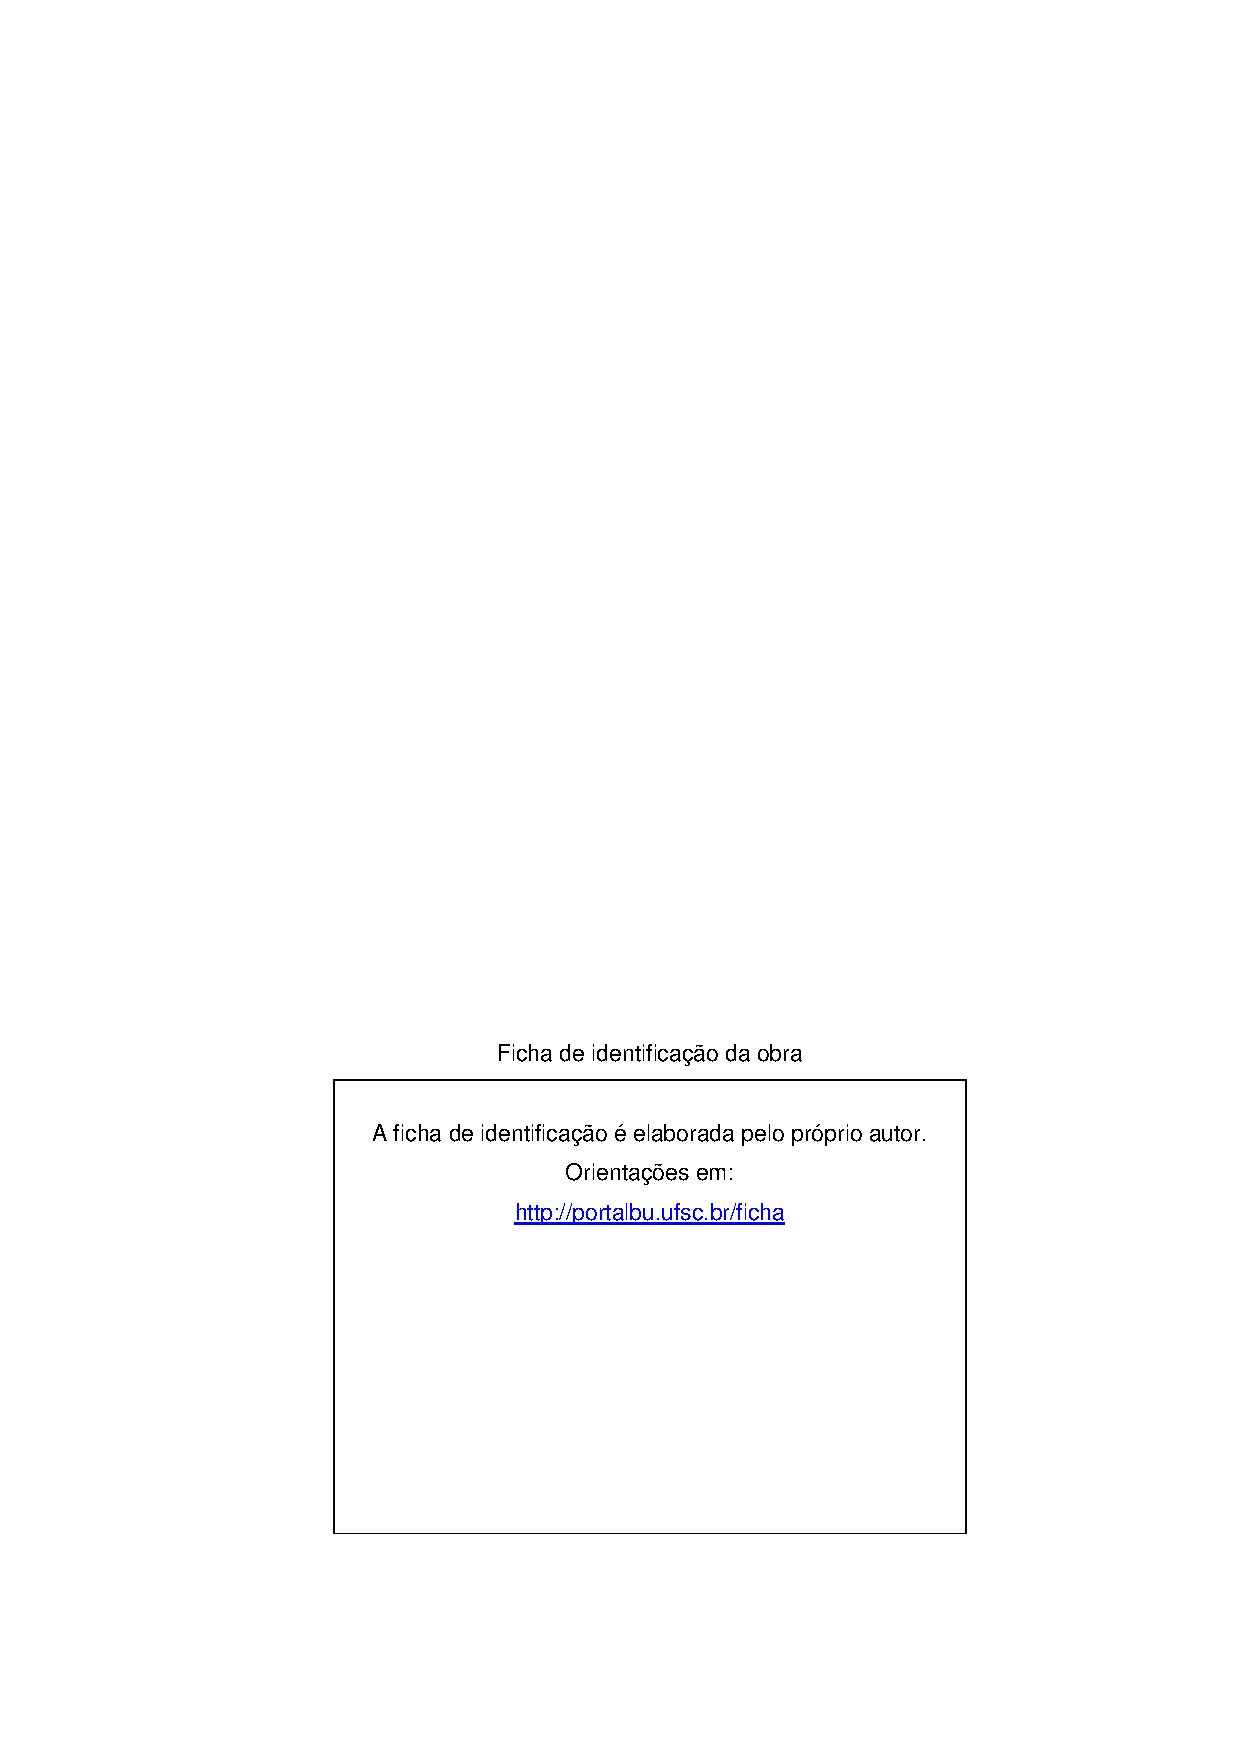
\includepdf{pre_textual/ficha_catalografica.pdf}
\end{fichacatalografica}

% Inserir folha de aprovação
\begin{folhadeaprovacao}
	\OnehalfSpacing
	\centering
	\imprimirautor\\%
	\vspace{24pt}		
	\textbf{\imprimirtitulo}%
	\ifnotempty{\imprimirsubtitulo}{:~\imprimirsubtitulo}\\%
	%		\vspace*{31.5pt}%3\baselineskip
	\vspace*{\baselineskip}
	%\begin{minipage}{\textwidth}
	Este Trabalho de Conclusão de Curso foi julgado adequado para obtenção do Título de ``\imprimirformacao'' e aprovado em sua forma final pelo Curso de Graduação em Engenharia de Controle e Automação.\\
	\vspace{12pt}
	\imprimirlocal, \imprimirdia~de~\imprimirmes~de~\imprimirano.\\
	
	\vspace*{18pt}
	\textbf{Banca Examinadora:}\\
	
	\vspace*{24pt}
	\assinatura{\OnehalfSpacing \imprimirbancaa}
	\vspace{6pt}
	Instituição xxxx\\
	
	\vspace*{24pt}
	\assinatura{\OnehalfSpacing \imprimirbancab}
	\vspace{6pt}
	Instituição xxxx\\
	
	\vspace*{24pt}
	\assinatura{\OnehalfSpacing \imprimirbancac}
	\vspace{6pt}
	Instituição xxxx\\
	
\end{folhadeaprovacao}

% Dedicatória
\ifnotempty{\imprimirdedicatoriatcc}{
\begin{dedicatoria}
	\vspace*{\fill}
	\noindent
	\begin{adjustwidth*}{}{5.5cm} 
		\raggedleft       
		\imprimirdedicatoriatcc
	\end{adjustwidth*}
\end{dedicatoria}
}

% Agradecimentos
\ifnotempty{\imprimiragradecimentostcc}{
\begin{agradecimentos}
	\imprimiragradecimentostcc
\end{agradecimentos}
}

% Epígrafe
\ifnotempty{\imprimirepigrafetcc}{
\begin{epigrafe}
	\vspace*{\fill}
	\imprimirepigrafetcc
\end{epigrafe}
}


% Resumo
\setlength{\absparsep}{18pt} % ajusta o espaçamento dos parágrafos do resumo
\begin{resumo}
	\SingleSpacing
	\imprimirresumotcc
	
	\textbf{Palavras-chave}: \imprimirpalavraschave
\end{resumo}

% Abstract
\begin{resumo}[Abstract]
	\SingleSpacing
	\imprimirabstracttcc
		
	\textbf{Keywords}: \imprimirkeywords
\end{resumo}


{%hidelinks
	\hypersetup{hidelinks}
	
	% inserir lista de figuras
	\pdfbookmark[0]{\listfigurename}{lof}
	\listoffigures*
	\cleardoublepage
	
	% inserir lista de quadros
	\ifnotempty{\verificaquadros}{
		\pdfbookmark[0]{\listofquadrosname}{loq}
		\listofquadros*
		\cleardoublepage
	}
	
	% inserir lista de tabelas
	\pdfbookmark[0]{\listtablename}{lot}
	\listoftables*
	\cleardoublepage
	
	% inserir lista de abreviaturas e siglas (devem ser declarados no preambulo)
	\ifnotempty{\verificasiglas}{
	\imprimirlistadesiglas
	}
	
	% inserir lista de símbolos (devem ser declarados no preambulo)
	\ifnotempty{\verificasimbolos}{
	\imprimirlistadesimbolos
	}
	
	% inserir o sumario
	\pdfbookmark[0]{\contentsname}{toc}
	\tableofcontents*
	\cleardoublepage
	
}%hidelinks

	% Elementos textuais
	\textual
	
	% 1 - Introdução
	% ----------------------------------------------------------
\chapter{Introdução}
% ----------------------------------------------------------
As mudanças climáticas têm intensificado a frequência e a severidade de eventos climáticos extremos, como chuvas intensas, secas prolongadas e inundações, impactando diretamente grandes centros urbanos e áreas rurais \cite{veja2024}. No Brasil, esses fenômenos têm se tornado mais frequentes, afetando a região Sul com inundações causadas por chuvas intensas que representam um desafio recorrente. As enchentes de 2024, que devastaram diversas cidades gaúchas, evidenciaram a necessidade de ferramentas eficazes para prever e mitigar os impactos de desastres naturais.

O problema abordado neste trabalho é a previsão do nível do Lago Guaíba, um dos principais mananciais de abastecimento de água de Porto Alegre e região metropolitana. \hl{No contexto do Lago Guaíba, a problemática é particularmente complexa devido à sua sensibilidade a chuvas intensas, tanto em seu leito principal quanto em seus afluentes, como os rios Jacuí, Caí, Gravataí e Sinos. As cheias de 2024 destacaram como a variabilidade climática e as contribuições dos afluentes amplificam as flutuações no nível do Guaíba, tornando essencial o desenvolvimento de modelos preditivos robustos} \cite{veja2024}.

A capacidade de prever o nível do rio é crucial para antecipar eventos de inundação, que podem causar perdas materiais significativas, deslocamento de populações e até mesmo mortes. A previsão do nível do rio, utilizando dados meteorológicos como variáveis preditoras, permite a elaboração de planos de evacuação, a alocação eficiente de recursos para mitigação de desastres e a proteção de infraestruturas críticas, contribuindo para a segurança e o bem-estar da população \cite{andrade2017}.

\hl{A importância de prever o nível de corpos d'água em geral, e do Lago Guaíba em Particular,} reside na possibilidade de reduzir os impactos socioeconômicos e ambientais causados pelas cheias. As inundações em Porto Alegre, como as observadas em 1941 e 2024, demonstram a vulnerabilidade da região a eventos climáticos extremos \cite{veja2024}. A elaboração de um modelo de previsão do nível do lago pode embasar decisões de políticas públicas e defesa civil, além de otimizar a gestão de recursos hídricos e outras aplicações que tangem a preservação e uso consciente do lago.

Apesar dos avanços em modelos hidrológicos e de previsão, as soluções atuais apresentam limitações que justificam a busca por novas abordagens. Algumas delas são computacionalmente custosas ou requerem dados extensivos que nem sempre estão disponíveis, dificultando sua implementação em tempo real \cite{andrade2017}.

Este trabalho propõe o uso de dados meteorológicos, como precipitação, temperatura, umidade e pressão atmosférica, combinados com técnicas de aprendizado de máquina, para prever o nível do rio, oferecendo uma ferramenta para a gestão de riscos de inundações.

\section{Objetivos}

O objetivo geral deste trabalho é desenvolver um modelo de previsão do nível do Lago Guaíba utilizando dados meteorológicos por meio de técnicas de aprendizado de máquina, especificamente a regressão Ridge.

Os objetivos específicos são:

\begin{itemize}
    \item Coletar e tratar dados meteorológicos e de níveis de rios relevantes para o modelo.
    \item Aplicar técnicas de pré-processamento de dados, incluindo limpeza e redução de dimensionalidade, para garantir a qualidade das informações.
    \item Implementar e treinar um modelo de regressão Ridge para prever o nível do Lago Guaíba com base nos dados meteorológicos.
    \item Avaliar o desempenho do modelo utilizando métricas de erro como MSE, RMSE, MAE e R².
    \item Analisar os resultados obtidos e propor ajustes para otimizar a previsão.
\end{itemize}

\section{Estrutura do trabalho}

\hl{O trabalho é constituído por 5 capítulos. No Capítulo 1 é apresentada a introdução, objetivos e estrutura do trabalho.}

\hl{O Capítulo 2 apresenta a fundamentação teórica sobre mudanças climáticas, catástrofes naturais, aprendizado de máquina e técnicas de regressão, incluindo conceitos de regressão linear e o modelo Ridge.}

\hl{No Capítulo 3 é apresentado o desenvolvimento, com ênfase na coleta de dados, pré-processamento, limpeza, redução, transformação e aplicação do modelo Ridge de previsão via \textit{script} na linguagem de programação Python.}

\hl{No Capítulo 4 são apresentados os resultados obtidos, incluindo gráficos de previsão, tabelas de métricas de desempenho para diferentes valores de alpha e proporções de divisão de dados, além de análise comparativa com estudos semelhantes. O Capítulo 5 trata da conclusão e discussões acerca do tema abordado e implementação desenvolvidaAo fim do trabalho encontram-se as referências.}

\hl{Dado que o presente trabalho envolve o desenvolvimento de um modelo preditivo baseado em dados meteorológicos e hidrológicos, os conceitos teóricos e metodológicos foram apresentados de forma prévia aos resultados. Consequentemente, as etapas de preparação de dados e implementação concentraram-se no desenvolvimento, com os resultados focados na avaliação do desempenho do modelo.}
	
	% 2 - Desenvolvimento
	% ----------------------------------------------------------
\chapter{Fundamentação Teórica}\label{cap:fundamentacaoTeorica}
% ----------------------------------------------------------
Esta seção apresenta os conceitos teóricos que sustentam o desenvolvimento do modelo preditivo para o nível do Lago Guaíba, com base em dados meteorológicos e na técnica de Regressão \textit{Ridge}. Inicialmente, aborda-se o impacto das mudanças climáticas e sua relação com eventos extremos, como as enchentes, destacando a relevância do monitoramento de rios em regiões vulneráveis, como o Rio Grande do Sul. Em seguida, são discutidos os princípios de aprendizado de máquina, com ênfase em abordagens supervisionadas, que formam a base para a modelagem proposta. Posteriormente, explora-se a teoria da regressão, incluindo a regressão linear simples e múltipla, e o método dos Mínimos Quadrados Ordinários, que são fundamentais para compreender a Regressão \textit{Ridge}. Por fim, detalha-se a técnica da regressão proposta para implementação, destacando sua capacidade de lidar com multicolinearidade e melhorar a generalização do modelo, essencial para a previsão precisa do nível do rio em cenários de alta variabilidade climática.

\section{As mudanças climáticas e as catástrofes naturais}

As grandes cidades brasileiras enfrentam desafios mais frequentes relacionados às mudanças climáticas, que agravam problemas como enchentes, inundações e deslizamentos. Projeções indicam que, até 2030, a mancha urbana de São Paulo pode aumentar em até 38\%, ampliando o risco para mais de 20\% das áreas de expansão urbana, que se tornarão suscetíveis a acidentes naturais. O aumento na frequência de eventos de chuvas intensas pode dobrar o número de dias com precipitação acima de 10 milímetros, agravando a vulnerabilidade da população, especialmente nas áreas periféricas e de menor infraestrutura \cite{Nobre2011}.

\subsection{Cenário de enchentes no sul do Brasil}

Com base no histórico das enchentes no Rio Grande do Sul, observa-se que os desastres relacionados ao excesso de chuvas não são um fenômeno recente. Desde 1941, o estado lida com eventos catastróficos, como a enchente que devastou Porto Alegre naquele ano, considerada uma das mais graves da história da cidade. Ao longo das décadas, esses episódios continuaram a ocorrer, expondo a vulnerabilidade da região diante de chuvas intensas e repentinas. A combinação de fatores naturais, como a geografia da região e os ciclos climáticos, aliado às ações humanas nocivas ao meio ambiente, contribui para a repetição e intensificação dessas tragédias \cite{veja2024}.

Em Santa Catarina, estado adjacente ao Rio Grande do Sul, as enchentes também são fenômenos recorrentes que, ao longo dos anos, têm causado impactos sociais, econômicos e ambientais. Um dos eventos mais recentes foi registrado em maio de 2024, quando o estado registrou vários dias com altos índices pluviométricos, levando ao transbordamento de rios, deslizamentos de terra e bloqueios em diversas rodovias \cite{g12024}.

\subsection{Dinâmica do Lago Guaíba}

O Lago Guaíba, principal manancial de abastecimento de água para a capital do Rio Grande do Sul e região, é alvo de estudo sobre diversos temas, incluindo sua hidrodinâmica e nível ao longo do ano. O Lago Guaíba apresenta flutuações significativas no volume de descarga, variando de 407 m³/s a 14.270 m³/s \cite{andrade2017}. Grande parte desta variação sofre influência dos rios que desemborcam no lago, como Rio Jacuí, que contribui com cerca de 84,6\% da água que aflui ao lago, além dos rios Sinos, Caí e Gravataí que contribuem com 7,5\%, 5,2\% e 2,7\%, respectivamente \cite{andrade2019}. 

Outro fator relevante em relação ao risco de enchentes do lago está no tempo de retenção das águas que chegam dos rios. Ao investigar os níveis de poluição do lago, devido a capital carecer de um tratamento de água 100\% efetivo, notou-se que grande parte da água do Guaíba fica retida por longos períodos, gerando baixa circulação e menor diluição de poluentes \cite{andrade2019}. Além do agravante da qualidade da água, esse comportamento faz com que o fluxo dos rios que chegam ao lago, em caso de um aumento atípico do volume, desencadeie enchentes que demoram para escoar, prejudicando ainda mais a população das cidades banhadas pelo lago. 

Na Figura \ref{fig:bacia_guaiba}, é mostrado alguns rios que fazem parte da bacia hidrográfica do Guaíba, e que influenciam diretamente no seu nível. À esquerda, percebe-se que um rio não é identificado, sendo este o Rio Jacuí, que contribui majoritariamente com o fluxo de água que aflui ao lago. Na Figura \ref{fig:bacia_guaiba_2}, fica evidente o motivo de seu maior impacto, dado sua extensão e largura maior que os demais rios. 

\begin{figure}[H]
	\caption{\label{fig:bacia_guaiba}Rios que desemborcam e influenciam no nível do Lago Guaíba.}
	\begin{center}
		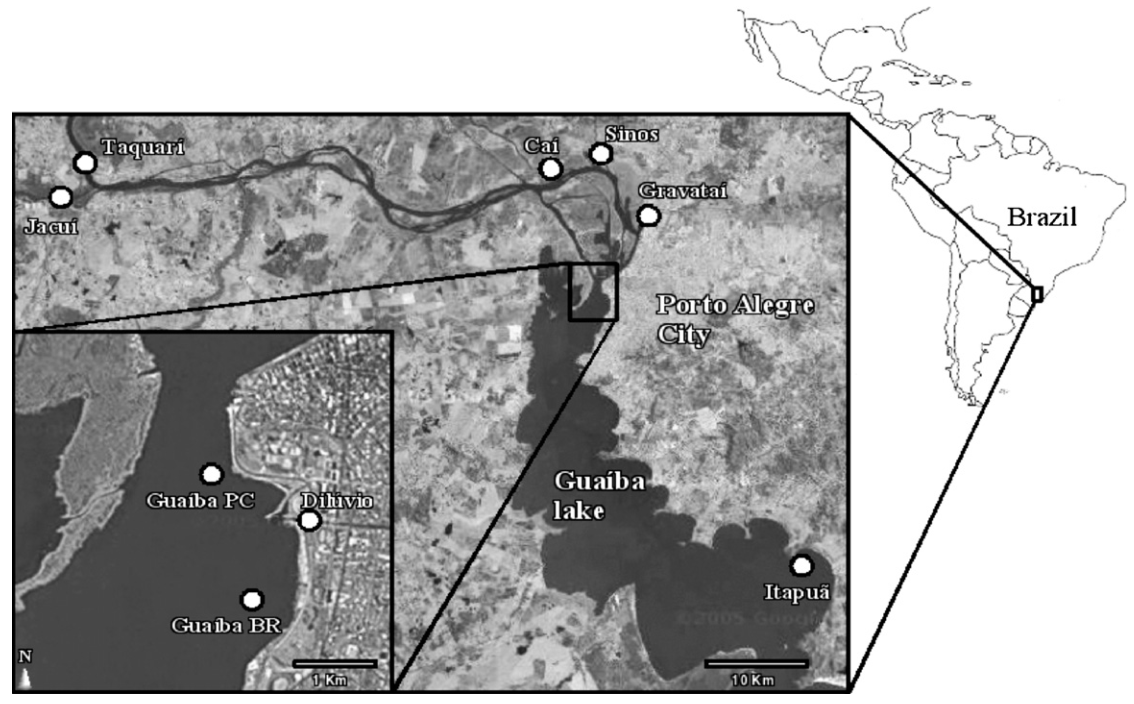
\includegraphics[scale=0.45]{figuras/bacia_lago_guaiba.png}
	\end{center}
	\fonte{\cite{g1_2024}.}
\end{figure}

\begin{figure}[H]
	\caption{\label{fig:bacia_guaiba_2}Rio Jacuí e seu desemboque no Lago Guaíba.}
	\begin{center}
		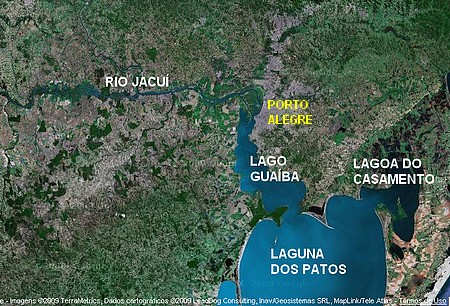
\includegraphics[scale=0.8]{figuras/lago_guaiba_2.jpg}
	\end{center}
	\fonte{\cite{portoimagem_2009}.}
\end{figure}

\section{Aprendizado de máquina}

Desde que os computadores foram inventados, criou-se o questionamento da possibilidade de fazê-los "pensar" de modo semelhante ao ser humano. Por meio desse avanço, diversas áreas sofreriam grandes transformações, uma vez que a capacidade da máquina aprender e aprimorar o seu conhecimento sobre determinado assunto traria melhorias e uma maior performance na atividade desejada \cite{carbonell1983}.

Embora os computadores ainda não alcancem o mesmo nível de aprendizado geral do ser humano, nos últimos anos, o \glsxtrfull{ML} se tornou realidade, com aplicações em diversos setores, agregando valor e conhecimento por meio de dados e informações antes tratados apenas por profissionais da área.

Esse conceito envolve a criação de sistemas que são capazes de aprender a partir de dados, identificando padrões e realizando previsões sem a necessidade de programação explícita. O principal objetivo do \gls{ML} é construir algoritmos que permitam que os computadores adquiram conhecimento e melhorem sua performance de forma autônoma, baseando-se em experiências passadas \cite{carbonell1983}.

\subsection{Categorias de aprendizado de máquina}

Os quatro principais tipos de \gls{ML} são: supervisionado, não supervisionado, semi-supervisionado e reforço \cite{saravanan2018}. Estes tipos de \gls{ML} são descritos a seguir:

\begin{itemize}
    \item Supervisionado: envolve a utilização de dados rotulados, no qual o modelo é treinado com entradas e saídas conhecidas para fazer previsões sobre novos dados;
    \item Não supervisionado: lida com dados não rotulados, onde o sistema busca encontrar padrões ou agrupamentos nos dados;
    \item Semissupervisionado: combina elementos de ambos os métodos, utilizando uma pequena quantidade de dados rotulados e uma grande quantidade de dados não rotulados, sendo útil em cenários onde a rotulação de dados é cara ou complexa;
    \item Aprendizado por reforço: se baseia em um sistema de recompensas e punições, onde o sistema interage com o ambiente e aprende a otimizar suas ações para alcançar um objetivo a partir de \textit{feedbacks} recebidos.
\end{itemize}

\section{Regressão}
\label{sec:regressao}

Para prever e entender a dinâmica de fenômenos estudados, a regressão, uma técnica de aprendizado supervisionado, modela relações entre variáveis dependentes e independentes por meio de métodos estatísticos \cite{soto2013}.

Em uma equação linear, uma variável independente, comumente representada pela letra $x$, caracteriza uma grandeza que está sendo manipulada durante um experimento. Dado esse comportamento, a variável $x$ não sofre influência de outras variáveis. A variável dependente, comumente representada pela letra $y$, caracteriza valores que estão diretamente associados à variável independente. Assim, de forma direta ou indireta, $x$ exerce influência sobre $y$.

A Figura \ref{fig:regressao_exemplo} ilustra um exemplo de regressão, mostrando a relação entre o índice de felicidade e a expectativa de vida em diversos países, conforme dados de \cite{helliwell2020}. Nesse contexto, o índice de felicidade é considerado a variável independente, enquanto a expectativa de vida é a variável dependente. Observando o gráfico, é possível perceber uma tendência de que países com maior índice de felicidade apresentam também uma expectativa de vida mais elevada. Assim, a regressão busca ajustar uma reta que, de forma aproximada, modela essa relação entre as variáveis, permitindo estimar valores de expectativa de vida a partir de valores do índice de felicidade. Tal reta pode ser representada pela equação linear mencionada anteriormente, e, caso disponível, a equação gerada pelos dados pode ser informada para descrever matematicamente a tendência observada na figura.

\begin{figure}[H]
	\caption{\label{fig:regressao_exemplo}Relação entre o índice de felicidade e expectativa de vida.}
	\begin{center}
		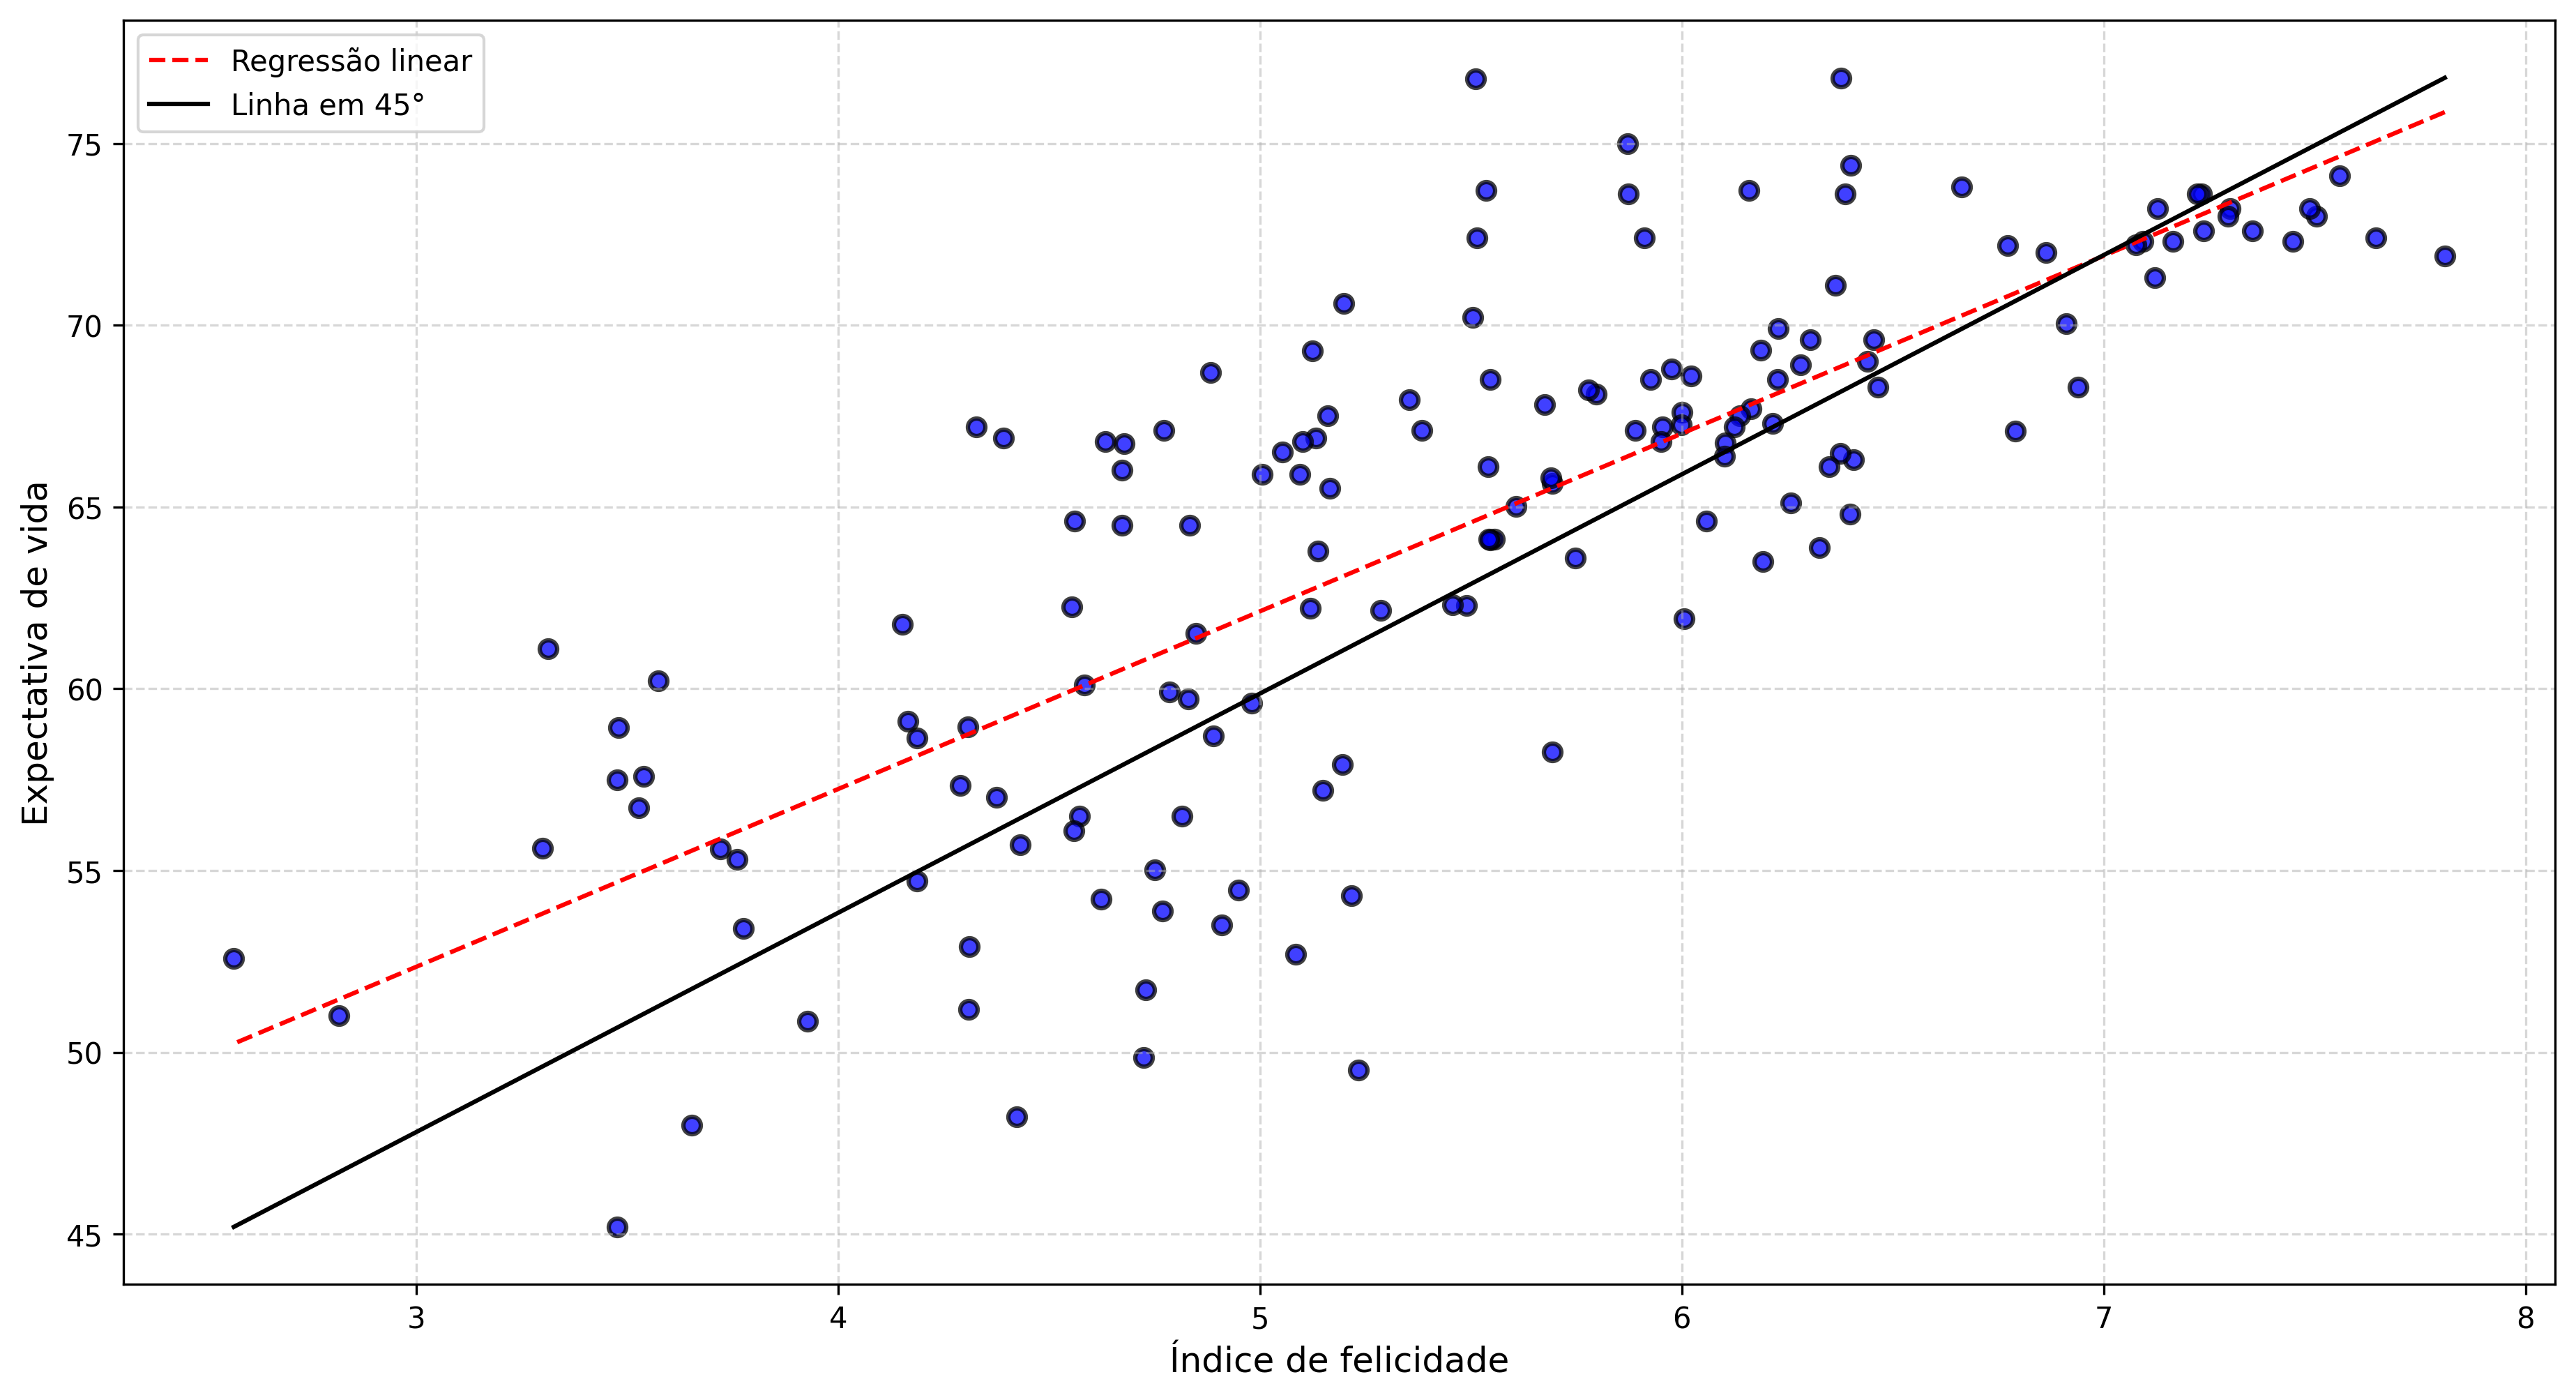
\includegraphics[scale=0.4]{figuras/happiness_world.png}
	\end{center}
	\fonte{\cite{helliwell2020}}
\end{figure}

Embora uma inferência inicial permita constatar uma correlação entre as variáveis da equação, a criação de um modelo de previsão necessita de métodos que comprovem a correlação pressuposta. Para determinar as relações entre as variáveis dependentes e independentes de um sistema, coeficientes de correlação são calculados, gerando valores que medem e comprovam estatisticamente o grau de correspondência dos fatores estudados. Uma das métricas de correlação mais utilizadas é o coeficiente de Pearson, que mede a associação linear entre duas variáveis \cite{kirch2008}. 

Esse coeficiente de correlação pode ser definido pela Equação \ref{eq:correlacao_person}, onde $n$ é o total de amostras, $\bar{x}$ e $\bar{y}$ são as médias aritméticas de ambas as variáveis. Os valores do coeficiente de Pearson variam entre -1 e 1, de tal forma que quanto mais próximos desses extremos, melhor correlacionadas estão as variáveis.

\begin{equation}
    r_{xy} = \frac{\sum_{i=1}^n (x_i - \bar{x})(y_i - \bar{y})}{\sqrt{\sum_{i=1}^n (x_i - \bar{x})^2 \sum_{i=1}^n (y_i - \bar{y})^2}}
    \label{eq:correlacao_person}
\end{equation}

A Figura \ref{fig:correlacoes} mostra alguns exemplos com gráficos de dispersão de variáveis com diferentes correlações.

\begin{figure}[H]
	\caption{\label{fig:correlacoes}Diferentes correlações entre variáveis.}
	\begin{center}
		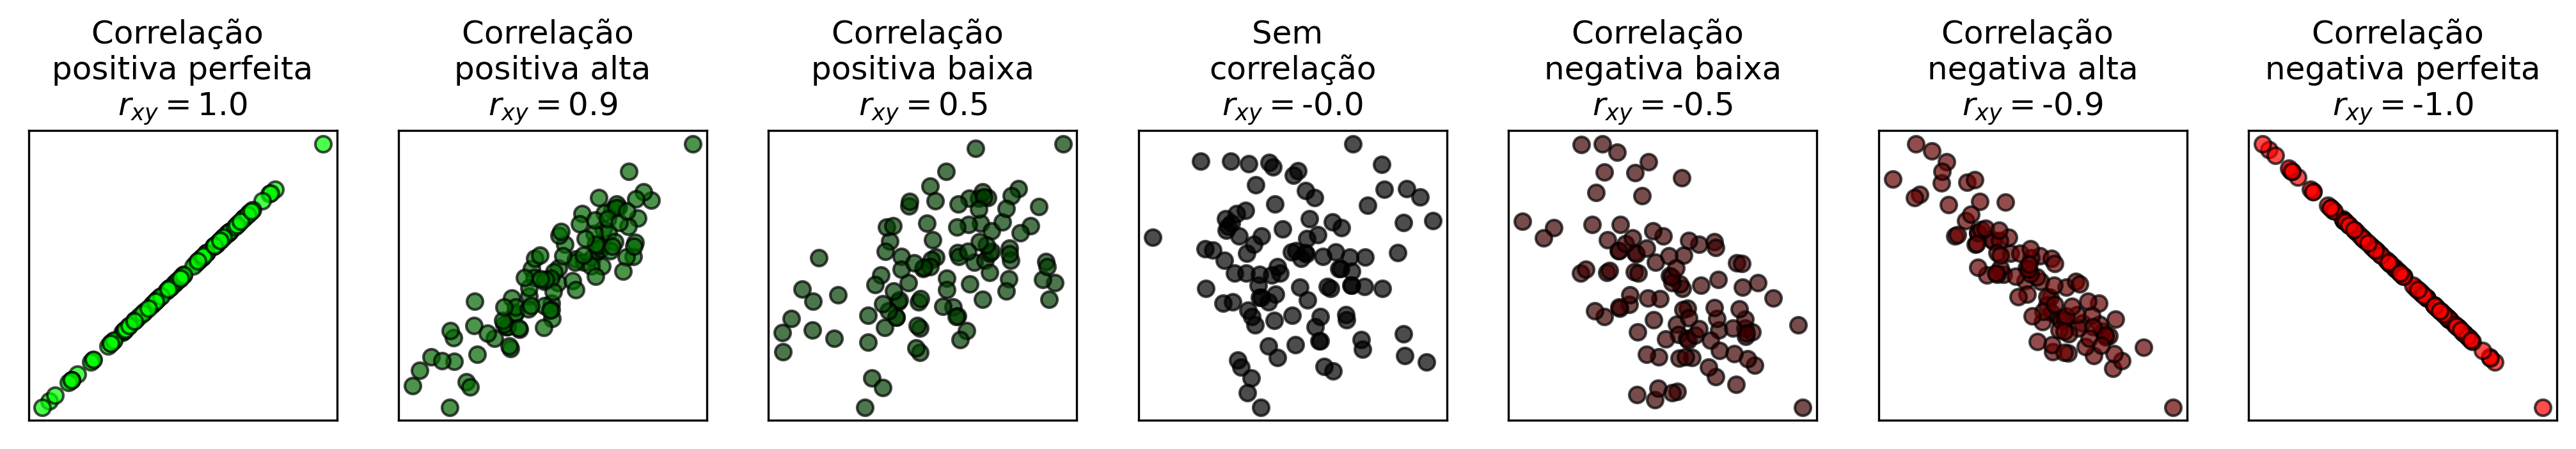
\includegraphics[scale=0.4]{figuras/correlations.png}
	\end{center}
	\fonte{\cite{helliwell2020}}
\end{figure}

Quando o coeficiente de correlação indica uma alta correlação entre variáveis independentes (por exemplo, dados meteorológicos) e a variável dependente (nível do Lago Guaíba), métodos mais simples de regressão podem ser utilizados para estimar valores não presentes no conjunto de dados, aproveitando a relação estatística identificada. No entanto, em casos onde o coeficiente indica baixa correlação entre as variáveis ou alta multicolinearidade entre as preditoras, métodos como a regressão Ridge se mostram vantajosos, pois incorporam uma penalidade (regularização L2) que reduz o impacto de variáveis menos relevantes ou correlacionadas, permitindo previsões mais robustas sem depender exclusivamente da força da correlação linear.

\section{Regressão Linear}
\label{sec:regressao-linear}

A regressão linear é um tipo específico de regressão que modela a relação entre uma variável independente e uma variável dependente, conforme citado em \ref{sec:regressao}. Amplamente utilizada em áreas como engenharia, ciências físicas, economia e ciências sociais, essa técnica assume que a relação entre as variáveis é linear, permitindo prever valores da variável dependente com base em uma ou mais variáveis independentes \cite{montgomery2012}.

A aplicação da técnica é relevante devido à sua simplicidade e capacidade de fornecer previsões baseadas em uma fórmula matemática interpretável. Além disso, o método é base para implementações de algoritmos na área de ciência de dados, otimizando o processamento de dados complexos e viabilizando a criação de modelos de previsão \cite{aws2024}.

O método de regressão linear é dividido em dois grupos, sendo eles: \glsxtrfull{RLS} e \glsxtrfull{RLM} \cite{montgomery2012}. A RLS tem como objetivo estabelecer uma relação entre duas variáveis através de uma função, cuja definição é dada por:

\begin{equation}
	y = \beta_0 + \beta_1 x + \varepsilon
	\label{eq:regressao_linear_simples}
\end{equation}

Onde $y$ é a variável dependente, $x$ a variável independente, enquanto $\beta_0$ e $\beta_1$ são coeficientes calculados pela regressão, que representam o valor de $y$ quando $x=0$ e o grau de inclinação da reta, respectivamente.

A RLM, embora seja semelhante à RLS, possui múltiplas variáveis preditoras, sendo definida por:

\begin{equation}
	y = \beta_0 + \beta_1 x_{1} + \beta_2 x_{2} + ... + \beta_k x_{k} + \varepsilon
	\label{eq:regressao_linear_multipla}
\end{equation}

Na equação \ref{eq:regressao_linear_multipla}, $y$ é a variável alvo, $x_{1}$ a $x_{k}$ as variáveis regressoras, e $\beta_0$ permanece sendo o coeficiente de intercepto do eixo Y enquanto $\beta_1$ a $\beta_n$ representam os coeficientes associados à n-ésima variável \cite{sassi2012}.

Nas equações \ref{eq:regressao_linear_simples} e \ref{eq:regressao_linear_multipla}, nota-se a presença do erro estatístico representado por $\varepsilon$, que é a diferença entre o valor observado e o valor previsto pela equação de regressão. Esse erro é considerado aleatório e contabiliza a falha do modelo ao tentar se aproximar do comportamento denotado pelos dados amostrados \cite{montgomery2012}.

Para compreender o modelo de regressão linear sob suas suposições fundamentais, considera-se que a variável independente $ x $ (por exemplo, precipitação meteorológica) é conhecida e usada para prever a variável dependente $ y $ (como o nível do Lago Guaíba). Sob essas condições, todos os termos do lado direito da equação $ y = \beta_0 + \beta_1 x + \varepsilon $ são conhecidos, exceto o erro $ \varepsilon $, que determina as propriedades estatísticas de $ y $. Assumindo que o erro $ \varepsilon $ tem média zero e variância constante $ \sigma^2 $ \cite{montgomery2012}, a resposta média para qualquer valor de $ x $ é dada por

\begin{equation}
	E(y \mid x) = \mu_{y \mid x} = E(\beta_0 + \beta_1x + \varepsilon) = \beta_0 + \beta_1x
\end{equation}

e a variância é dada por:

\begin{equation}
	Var (y \mid x) = \sigma_{y \mid x}^2 = Var(\beta_0 + \beta_1x + \varepsilon) = \sigma^2
\end{equation}

Desse modo, o modelo de regressão verdadeiro $\mu_{y \mid x} = \beta_0 + \beta_1x$ representa uma linha de valores médios, ou seja, a altura da linha de regressão em qualquer valor de x corresponde ao valor esperado de y para aquele x.

Para exemplificar as suposições da regressão linear, considera-se um modelo ilustrado pela Figura 3a, onde a média condicional é $ \mu_{y|x} = 3.5 + 2x $ e a variância do erro é $ \sigma^2 = 2 $. O erro $ \varepsilon $ segue uma distribuição normal, descrevendo a variação aleatória em torno da média. Como $ y $ é a soma de uma componente linear $ \beta_0 + \beta_1 x $ (a média) e o erro $ \varepsilon $, normalmente distribuído, $ y $ também segue uma distribuição normal. Por exemplo, para um valor específico da variável independente $ x = 10 $, $ y $ terá uma distribuição normal com média $ \mu_{y|x} = 3.5 + 2(10) = 23.5 $ e variância $ \sigma^2 = 2 $. Quanto menor a variância, mais próximos os pontos estarão da linha de regressão; uma variância maior resulta em maior dispersão em relação à linha de regressão \cite{montgomery2012}.

A maioria dos fênomenos nos quais se deseja obter a função que descreve o seu comportamento resulta em uma aproximação funcional através das variáveis de interesse. Essas relações funcionais frequentemente baseiam-se em teorias físicas, químicas ou de engenharia e ciências, ou seja, no conhecimento do mecanismo subjacente. Na Figura \ref{fig:regressao_linear_aprox_relacao_complexa}, é mostrada uma relação entre as variáveis $x$ e $y$ relativamente complexa, mas que pode ser aproximada de por uma equação de regressão linear, com um erro relativamente baixo.

\begin{figure}[H]
	\centering
	\caption{Interpretação de uma regressão linear}
	\begin{subfigure}{0.4\textwidth}
	  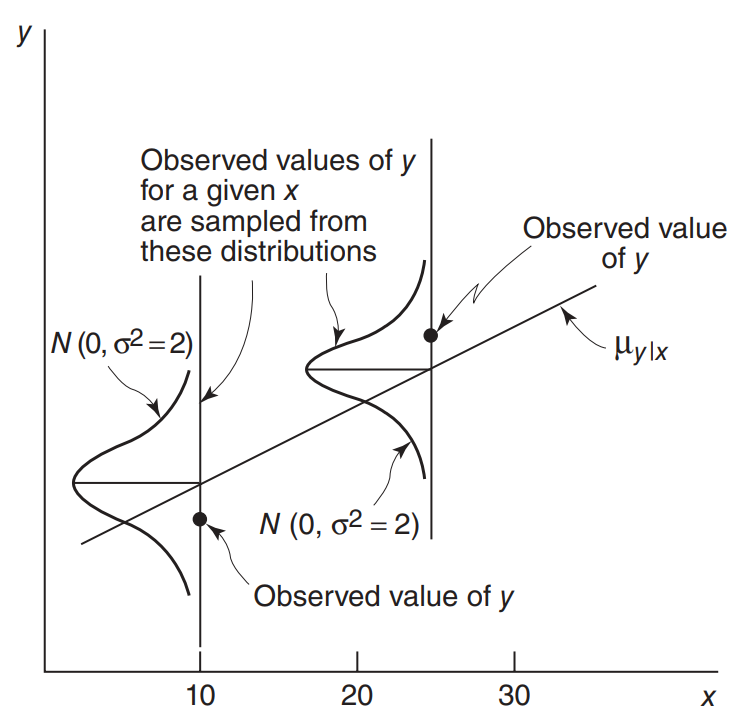
\includegraphics[width=\linewidth]{figuras/how_observations_are_generated_in_linear_regression.png}
	  \caption{Como as observações são geradas na regressão linear}
	  \label{fig:observacoes_regressao_linear}
	\end{subfigure}
	\hspace{0.5cm}
	\begin{subfigure}{0.4\textwidth} 
		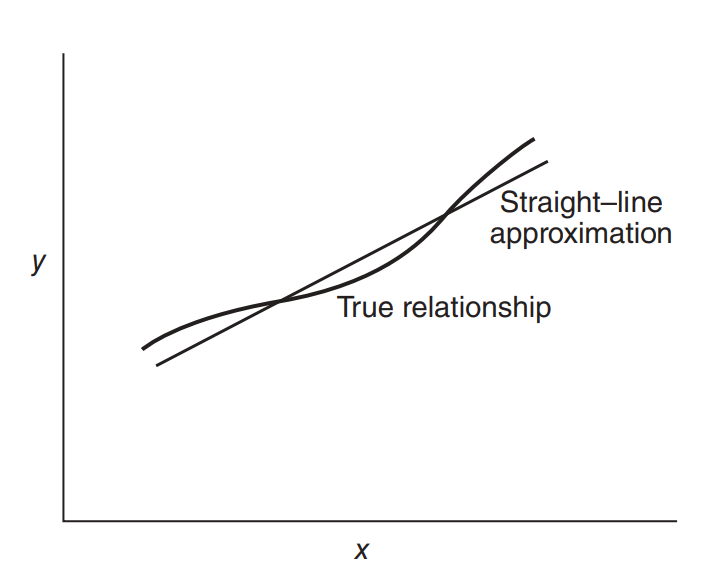
\includegraphics[width=\linewidth]{figuras/linear_regression_approximation_of_a_complex_relationship.png}
		\caption{Regressão linear como aproximação de uma relação complexa}
		\label{fig:regressao_linear_aprox_relacao_complexa}
	\end{subfigure}
	\label{fig:comportamento_regressao_linear}
	\fonte{\cite{montgomery2012}}
\end{figure}

Contudo, em alguns casos, quando a dinâmica do modelo a ser estimada passa a ter um grau de complexidade maior, como é o caso da Figura \ref{fig:aproximacao_linear_complexa}, utlizar uma RLS pode implicar em erros que extrapolam a tolerância exigida no estudo. Nesses cenários, utilizar uma função de regressão linear em intervalos específicos, ou seja, uma RLM, se torna uma alternativa plausível, tendo em vista que, para intervalos menores onde a dinâmica do fênômeno é mais linear, a regressão apresenta um erro menor, como mostra a Figura \ref{fig:intervalo_aplicacao_rls}.

\begin{figure}[H]
	\centering
	\caption{Situações de inadequação da RLS}
	\begin{subfigure}{0.4\textwidth}
	  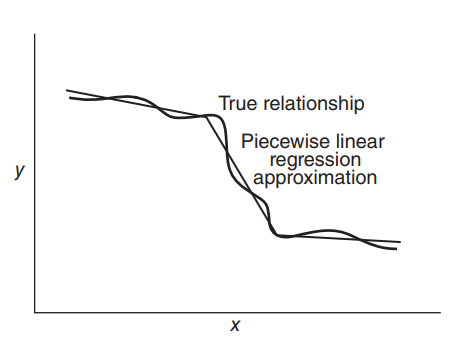
\includegraphics[width=\linewidth]{figuras/piecewise_linear_approximation.png}
	  \caption{Aproximação Linear complexa}
	  \label{fig:aproximacao_linear_complexa}
	\end{subfigure}
	\hspace{0.5cm}
	\begin{subfigure}{0.4\textwidth} 
		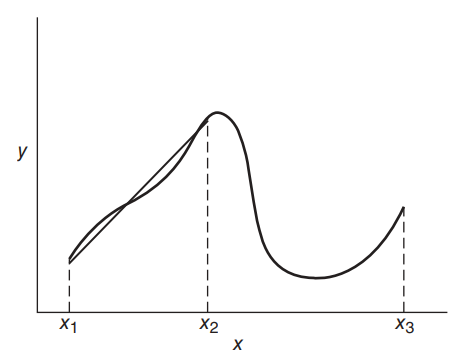
\includegraphics[width=\linewidth]{figuras/danger_extrapolation_regression.png}
		\caption{Intervalo de aplicação da RLS}
		\label{fig:intervalo_aplicacao_rls}
	\end{subfigure}
	\label{fig:comportamento_regressao_linear}
	\fonte{\cite{montgomery2012}}
\end{figure}

Partindo desses conceitos, para implementação de modelos de regressão linear e múltipla, o método dos Mínimos Quadrados Ordinários se apresenta como uma abordagem para estimar a melhor regressão dos pontos observados, encontrando uma reta com o menor erro entre as amostras e os valores da função estudada.

\section{Método dos quadrados ordinários}

O método \glsxtrfull{MQO} atua como uma ferramenta estatística, visando estimar a relação entre uma variável dependente e uma ou mais variáveis independentes \cite{Alkama2020}, permitindo encontrar os coeficientes desejados para o funcionamento do modelo.

Para obter uma regressão que se aproxima da dinâmica analisada, o método visa minimizar a \glsxtrfull{RSS}, denotado pela equação \ref{eq:rss_rls} para os casos de RLS (isto é, quando há apenas uma variável independente).

\begin{equation}
	RSS = \sum_{i=1}^{n} \left(y_i - \beta_0 - \beta_1x_{i}\right)^2
	\label{eq:rss_rls}
\end{equation}

Para o caso de \gls{RLM}, utiliza-se a equação \ref{eq:rss_rlm}, onde:

\begin{itemize}
    \item $y_i$ é uma variável aleatória e representa o valor da variável resposta (variável dependente) na i-ésima observação
    \item $x_{ij}$ representa o valor da j-ésima variável explicativa (variável independente, variável regressora) na i-ésima observação. Nota-se que podem existir $p$ variáveis independentes (sendo $p \geq 1$) para uma variável independente; 
    \item $\beta_{0}$ e $\beta_{j}$ são os parâmetros do modelo que serão estimados, e que definem a reta de regressão
\end{itemize}

\begin{equation}
    RSS = \sum_{i=1}^{n} \left(y_i - \beta_0 - \sum_{j=1}^{p}\beta_jx_{ij}\right)^2
	\label{eq:rss_rlm}
\end{equation}

Para minimizar a SSR em um caso de RLS, por exemplo, são calculadas as derivadas parciais de $\beta_0$ e $\beta_1$, igualando ambas a zero.

Derivada em relação à $\beta_0$:

\begin{equation}
	\frac{\partial RSS}{\partial \beta_0} = -2 \sum_{i=1}^n (y_i - \beta_0 - \beta_1 x_i) = 0
\end{equation}

simplificando:

\begin{gather*}
	\sum_{i=1}^n (y_i - \beta_0 - \beta_1 x_i) = 0 \\
	\sum_{i=1}^n y_i - n \beta_0 - \beta_1 \sum_{i=1}^n x_i = 0
\end{gather*}

divindindo por $n$:

\begin{gather*}
	\frac{\sum_{i=1}^n y_i}{n} - \beta_0 - \beta_1 \frac{\sum_{i=1}^n x_i}{n} = 0 \\
	\bar{y} - \beta_0 - \beta_1 \bar{x} = 0
\end{gather*}

onde $\bar{y}$ e $\bar{x}$ são as médias amostrais de $y$ e $x$, respectivamente. Assim, a equação pode ser reescrita como:

\begin{equation}
	\beta_0 = \bar{y} - \beta_1 \bar{x}
	\label{eq:beta0}
\end{equation}

Derivada em relação à $\beta_1$:

\begin{equation}
	\frac{\partial SSR}{\partial \beta_1} = -2 \sum_{i=1}^n x_i (y_i - \beta_0 - \beta_1 x_i) = 0
\end{equation}

substituindo $\beta_0$ na equação:


\begin{gather*}
	\sum_{i=1}^n x_i (y_i - (\bar{y} - \beta_1 \bar{x}) - \beta_1 x_i) = 0 \\
	\sum_{i=1}^n x_i (y_i - \bar{y} + \beta_1 \bar{x} - \beta_1 x_i) = 0 \\
	\sum_{i=1}^n x_i (y_i - \bar{y}) + \sum_{i=1}^n x_i (\beta_1 \bar{x} - \beta_1 x_i) = 0 \\
	\sum_{i=1}^n x_i (y_i - \bar{y}) - \beta_1 \sum_{i=1}^n x_i (x_i - \bar{x}) = 0
\end{gather*}

sabendo que:

\begin{gather*}
	\sum_{i=1}^n x_i (x_i - \bar{x}) = \sum_{i=1}^n (x_i - \bar{x})^2
\end{gather*}

e

\begin{gather*}
	\sum_{i=1}^n x_i (y_i - \bar{y}) = \sum_{i=1}^n (x_i - \bar{x})(y_i - \bar{y})	
\end{gather*}

portanto:

\begin{gather*}
	\sum_{i=1}^n (x_i - \bar{x})(y_i - \bar{y}) = \beta_1 \sum_{i=1}^n (x_i - \bar{x})^2
\end{gather*}

\begin{equation}
	\beta_1 = \frac{\sum_{i=1}^n (x_i - \bar{x})(y_i - \bar{y})}{\sum_{i=1}^n (x_i - \bar{x})^2}
\end{equation}




Desse modo, a partir de um problema onde uma ou mais entradas geram amostras que resultam em uma saída, torna-se possível estimar uma função que melhor representa seu comportamento, minimizando ao máximo o valor da soma residual dos quadrados entre os pontos amostrais e a curva do modelo. 

\begin{table}[h!]
\centering
\begin{tabular}{|c|c|}
\hline
\textbf{Variável Independente} & \textbf{Variável Dependente} \\
\hline
0,38 & 6,98 \\
0,41 & 4,05 \\
0,44 & 5,52 \\
0,59 & 6,93 \\
0,98 & 6,57 \\
1,04 & 6,41 \\
1,22 & 8,27 \\
1,53 & 6,93 \\
1,74 & 8,89 \\
1,84 & 9,31 \\
\hline
\end{tabular}
\caption{Tabela de Valores Ordenados: Variável Independente vs. Variável Dependente}
\label{tab:valores_exemplo_mqo}
\end{table}

A Tabela \ref{tab:valores_exemplo_mqo} apresenta um exemplo de dados amostrais, onde a variável independente é representada pela primeira coluna e a variável dependente pela segunda coluna. A partir desses dados, é possível aplicar o método dos mínimos quadrados para encontrar os coeficientes que melhor se ajustam à reta de regressão linear.

Ao aplicar o método para resolver um problema, como é o caso da Tabela \ref{tab:valores_exemplo_mqo}, todos os pontos amostrados são utilizados para encontrar a reta que melhor se ajusta aos dados. Contudo, visando mostrar como a dinâmica de regressão utilizando MQO funciona, nos passos seguintes, as amostras são consideradas de forma cumulativa, alterando a cada iteração os valores de $\beta_0$ e $\beta_1$, até que a reta de regressão linear se ajuste aos dados amostrais.

Passo 1: Apenas o ponto (0.44, 5.52)

Com um único ponto, a reta passa exatamente por sobre o mesmo, porém o método MQO exige pelo menos dois pontos para definir uma inclinação. Assim, assume-se uma reta horizontal ao usar o ponto como base inicial.

\begin{gather*}
	\beta_0 = 5.52, \quad \beta_1 = 0
\end{gather*}


\begin{figure}[H]
	\caption{\label{fig:mqo_1}Passo 1 da regressão linear pelo método MQO.}
	\begin{center}
		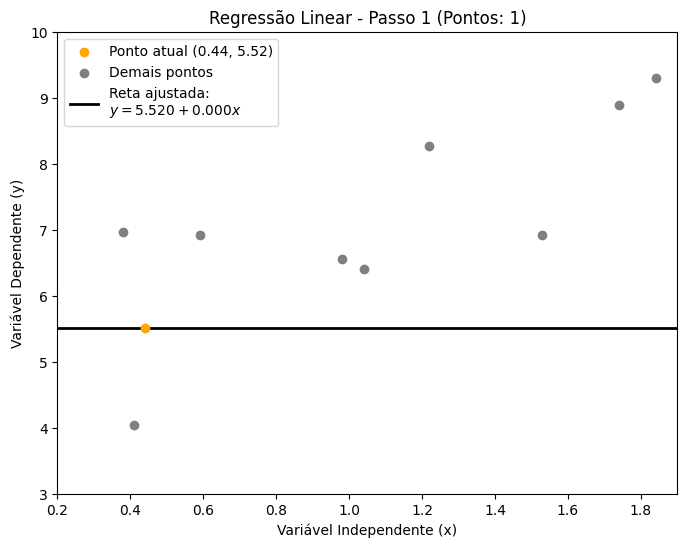
\includegraphics[scale=0.5]{figuras/RL_step_1.png}
	\end{center}
	\fonte{Autor.}
\end{figure}

Passo 2: Adiciona-se (1.74, 8.89)
\\ \\
n=2

\begin{gather*}
	\bar{x} = \frac{0.44 + 1.74}{2} = 1.09, \quad \bar{y} = \frac{5.52 + 8.89}{2} = 7.205
\end{gather*}

\begin{align*}
	\sum (x_i - \bar{x})(y_i - \bar{y}) &= \\
	(0.44 - 1.09)(5.52 - 7.205) + (1.74 - 1.09)(8.89 - 7.205) &=\\
	(-0.65)(-1.685) + (0.65)(1.685) &= \\
	1.09525 + 1.09525 &= 2.1905
\end{align*}

\begin{align*}
	\sum (x_i - \bar{x})^2 &=\\ 
	(0.44 - 1.09)^2 + (1.74 - 1.09)^2 &=\\
	0.4225 + 0.4225 &= 0.845
\end{align*}

\begin{gather*}
	\beta_0 = \frac{2.1905}{0.845} \approx 2.5923, \quad \beta_1 = 7.205 - 2.5923 \cdot 1.09 \approx 4.3795\\ \\
	\hat{y} = 4.3795 + 2.5923x
\end{gather*}

\begin{figure}[H]
	\caption{\label{fig:mqo_2}Passo 2 da regressão linear pelo método MQO.}
	\begin{center}
		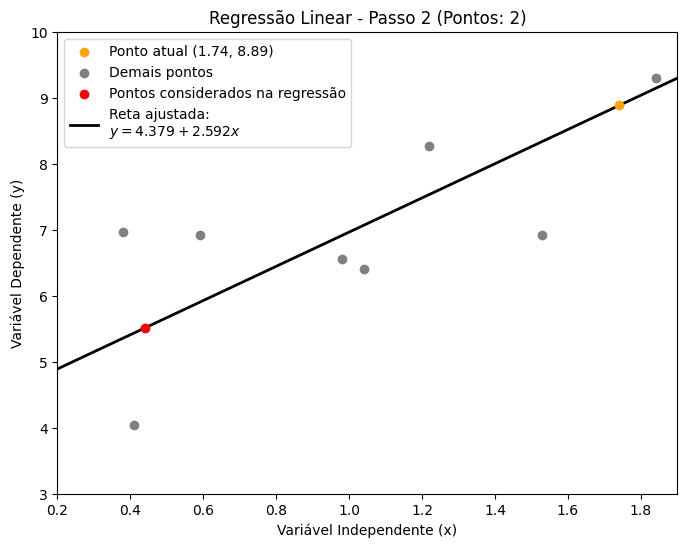
\includegraphics[scale=0.5]{figuras/RL_step_2.png}
	\end{center}
	\fonte{Autor.}
\end{figure}

Passo 3: Adiciona (0.41, 4.05)
\\ n = 3

\begin{gather*}
	\bar{x} = \frac{0.44 + 1.74 + 0.41}{3} = 0.8633, \quad \bar{y} = \frac{5.52 + 8.89 + 4.05}{3} = 6.1533 \\
	\sum (x_i - \bar{x})(y_i - \bar{y}) = \\ 
	(0.44 - 0.8633)(5.52 - 6.1533) + \\
	(1.74 - 0.8633)(8.89 - 6.1533) + \\
	(0.41 - 0.8633)(4.05 - 6.1533) \approx  \\
	0.268 + 2.399 + 0.953 = 3.62 \\ \\
	\sum (x_i - \bar{x})^2 = (0.44 - 0.8633)^2 + (1.74 - 0.8633)^2 + (0.41 - 0.8633)^2 \\
	\approx 0.179 + 0.769 + 0.205 = 1.153 \\
	\beta_0 = \frac{3.62}{1.153} \approx 3.1402 \\
	\beta_1 = 6.1533 - 3.1402 \cdot 0.8633 \approx 6.1533 - 2.711 = 3.4423 \\ \\
	\hat{y} = 3.4423 + 3.1402x
\end{gather*}

\begin{figure}[H]
	\caption{\label{fig:mqo_2}Passo 3 da regressão linear pelo método MQO.}
	\begin{center}
		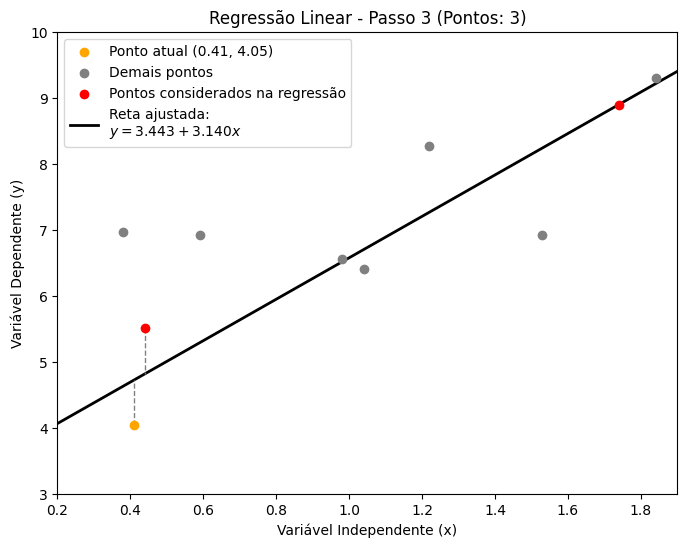
\includegraphics[scale=0.5]{figuras/RL_step_3.png}
	\end{center}
	\fonte{Autor.}
\end{figure}

Para os demais passos, o mesmo cálculo é realizado, onde a média amostral e os coeficientes são recalculados a cada iteração, conforme os pontos são adicionados.

\begin{figure}[H]
	\centering
	\caption{Iterações da aplicação do método MQO}
	\begin{subfigure}{0.4\textwidth}
	  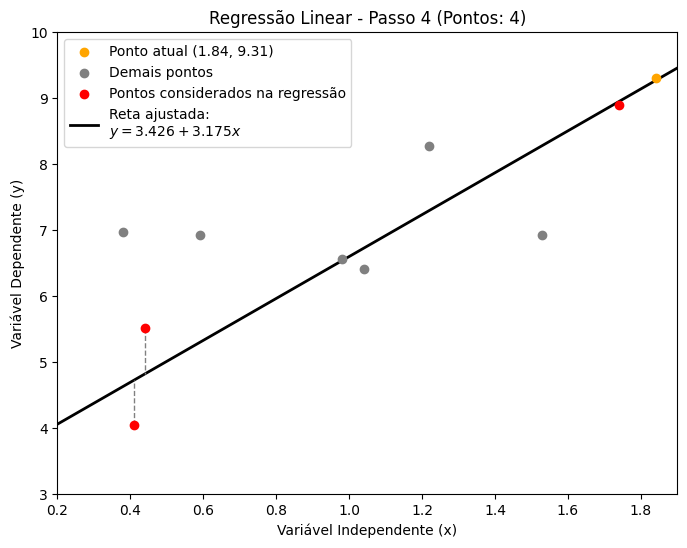
\includegraphics[width=\linewidth]{figuras/RL_step_4.png}
	  \caption{$n = 4$ | $y = 3,426 + 3,175x$}
	  \label{fig:mqo_4}
	\end{subfigure}
	\hspace{0.5cm}
	\begin{subfigure}{0.4\textwidth} 
		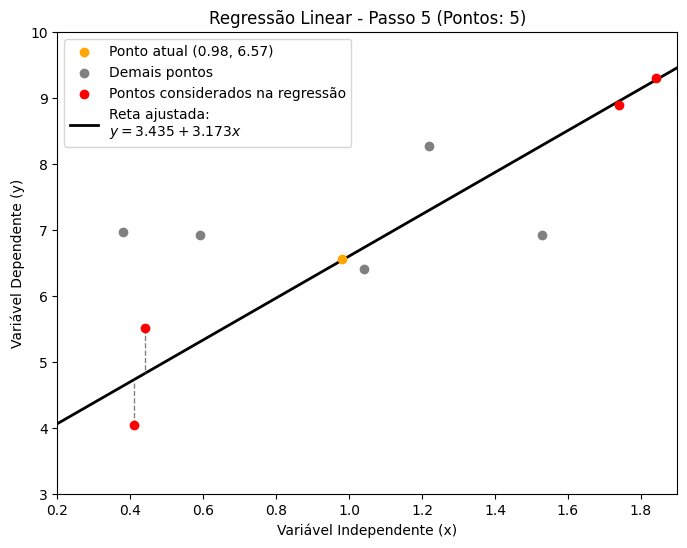
\includegraphics[width=\linewidth]{figuras/RL_step_5.png}
		\caption{$n = 5$ | $y = 3,435 + 3,173x$}
		\label{fig:intervalo_aplicacao_rls}
	\end{subfigure}
	\label{fig:mqo_5}
	\begin{subfigure}{0.4\textwidth} 
		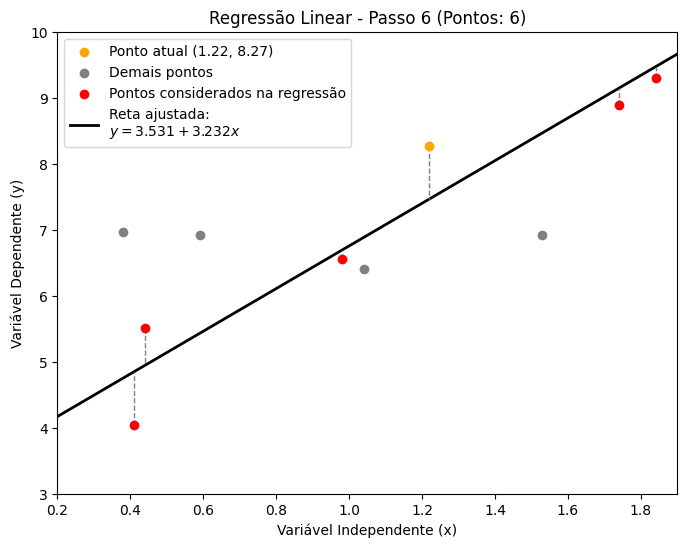
\includegraphics[width=\linewidth]{figuras/RL_step_6.png}
		\caption{$n = 6$ | $y = 3,531 + 3,232x$}
		\label{fig:intervalo_aplicacao_rls}
	\end{subfigure}
	\label{fig:mqo_6}
	\begin{subfigure}{0.4\textwidth} 
		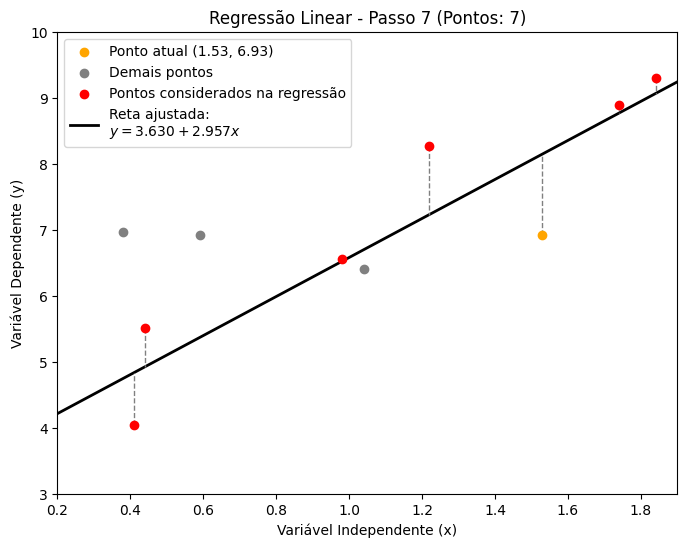
\includegraphics[width=\linewidth]{figuras/RL_step_7.png}
		\caption{$n = 7$ | $y = 3,630 + 2,957x$}
		\label{fig:intervalo_aplicacao_rls}
	\end{subfigure}
	\label{fig:mqo_7}
	\begin{subfigure}{0.4\textwidth} 
		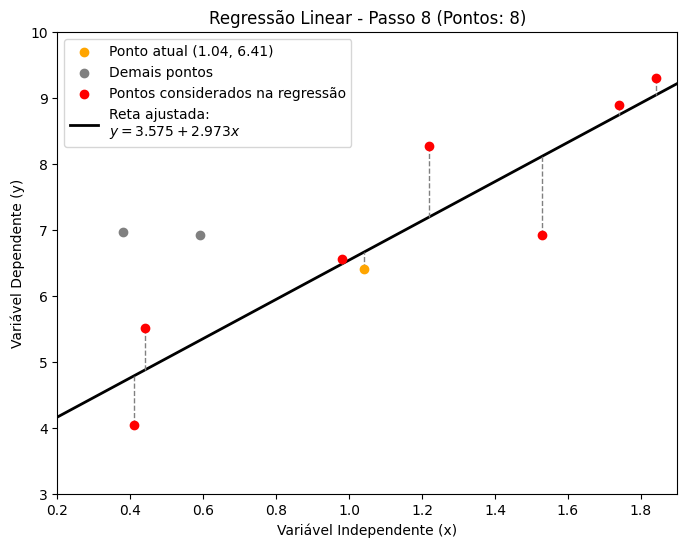
\includegraphics[width=\linewidth]{figuras/RL_step_8.png}
		\caption{$n = 8$ | $y = 3,575 + 2,973x$}
		\label{fig:intervalo_aplicacao_rls}
	\end{subfigure}
	\label{fig:mqo_8}
	\begin{subfigure}{0.4\textwidth} 
		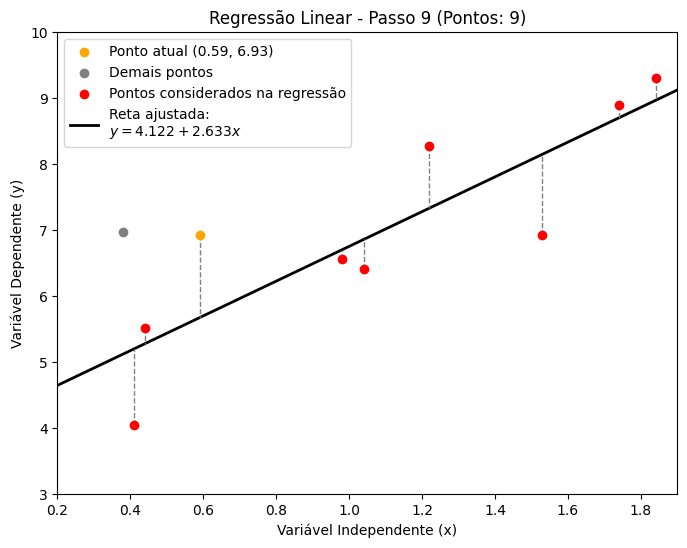
\includegraphics[width=\linewidth]{figuras/RL_step_9.png}
		\caption{$n = 9$ | $y = 4,122 + 2,633x$}
		\label{fig:intervalo_aplicacao_rls}
	\end{subfigure}
	\label{fig:mqo_9}
	\fonte{Autor.}
\end{figure}

Assim, a cada ponto selecionado da amostra, é calculada a derivada parcial da função estimada, determinando novos coeficientes que melhor descrevem a reta entre as amostras. Dado que não é possível estimar uma reta que passe sobre todos os pontos amostrados, os resíduos representados pelas linhas tracejadas na Figura \ref{fig:mqo_10} são definidos de tal modo que o somatório dos seus quadrados seja o menor possível.


\begin{figure}[H]
	\caption{\label{fig:mqo_10}Passo 10 da regressão linear pelo método MQO.}
	\begin{center}
		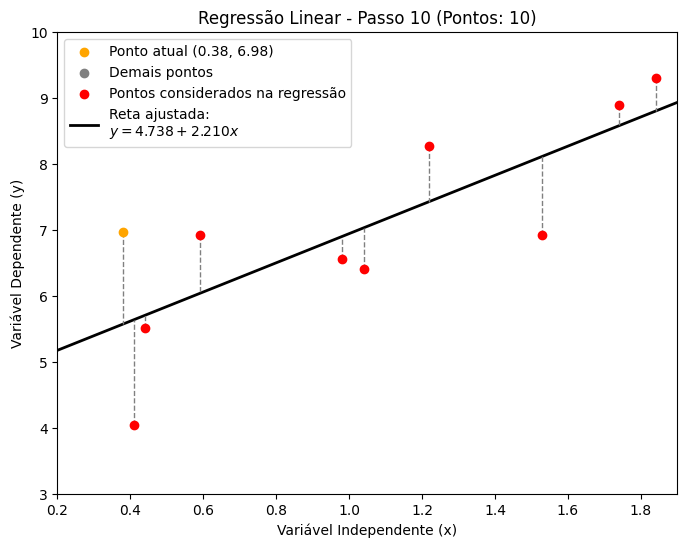
\includegraphics[scale=0.6]{figuras/RL_step_10.png}
	\end{center}
	\fonte{Autor.}
\end{figure}


\section{Modelo Ridge}
\label{sec:regressao-ridge}

A Regressão Ridge é uma técnica de regularização estatística amplamente utilizada em modelos de regressão linear para abordar problemas de sobreajuste (ou \textit{overfitting}, quando o modelo se ajusta demais aos dados de treinamento, perdendo a capacidade de prever dados fora da base passada para o modelo) e multicolinearidade entre variáveis preditoras \cite{McDonald:2009:RR}. Essa técnica, também conhecida como regularização L2, é particularmente eficaz em cenários onde o número de variáveis preditoras é grande ou quando essas variáveis apresentam alta correlação, o que pode levar a estimativas de coeficientes instáveis e de baixa generalização.

Conforme visto em \ref{sec:regressao-linear}, na regressão linear tradicional, o objetivo é minimizar o valor de \gls{RSS}, que mede a diferença entre os valores observados e os valores previstos pelo modelo. A função de perda é dada por:

\begin{equation}
	RSS = \sum_{i=1}^{n} (y_i - \hat{y}_i)^2
\end{equation}
\\

\noindent onde $y_i$ são os valores observados, $\hat{y}_i$ são os valores previstos, e $n$ é o número de observações. No entanto, em cenários com multicolinearidade (alta correlação entre variáveis preditoras) ou um grande número de preditores, o modelo pode se ajustar excessivamente aos dados de treinamento, resultando em alta variância e baixa performance em dados não vistos. A Regressão Ridge trata esse problema ao adicionar um termo de penalidade à função de perda, proporcional à soma dos quadrados dos coeficientes de regressão. 

A função objetivo da Regressão Ridge é:

\begin{equation}
	RSS_{L2} = \sum_{i=1}^{n} (y_i - \hat{y}_i)^2 + \alpha \sum_{j=1}^{p} \beta_j^2
\end{equation}

No contexto da biblioteca \textit{Scikit-learn} em Python, a classe Ridge implementa a Regressão Ridge. O parâmetro \textit{alpha} define a força da regularização: valores maiores de $\alpha$ resultam em coeficientes mais próximos de zero, enquanto valores menores permitem que o modelo se aproxime da regressão linear ordinária. A escolha adequada de 
$\alpha$ é crucial para evitar tanto o \textit{overfitting} quanto o \textit{underfitting} (quando o modelo é muito simples para capturar os padrões dos dados). \cite{ScikitLearnRidge2025}.

Além de impactar a função RSS, a Regressão Ridge altera o processo de busca pelos coeficientes $\beta$ que definem a reta (ou hiperplano, no caso de múltiplas variáveis) que melhor representa a regressão.

Na regressão linear tradicional, os coeficientes $\beta$ são encontrados minimizando-se apenas a soma dos quadrados dos resíduos, resultando em uma solução exata obtida pela equação normal:

\begin{equation}
	\hat{\boldsymbol\beta} = (\mathbf{X}^\top \mathbf{X})^{-1} \mathbf{X}^\top \mathbf{y}
\end{equation}

\noindent onde $\mathbf{X}$ é a matriz de variáveis independentes e $\mathbf{y}$ é o vetor de variáveis dependentes \cite{montgomery2012}.

Entretanto, quando há multicolinearidade ou grande número de variáveis, a matriz $\mathbf{X}^\top \mathbf{X}$  pode se tornar quase singular, causando coeficientes instáveis e de grande magnitude. A Regressão Ridge resolve isso ao adicionar o termo de penalização $\alpha \sum_{j=1}^{p}\beta_{j}^2$, modificando a equação normal para:

\begin{equation}
	\hat{\boldsymbol\beta}_{ridge} = (\mathbf{X}^\top \mathbf{X} + \alpha \mathbf{I})^{-1} \mathbf{X}^\top \mathbf{y}
\end{equation}

\noindent \cite{ScikitLearnRidge2025}.

Geometricamente, a regularização imposta pela Ridge faz com que a busca pela solução deixe de se restringir apenas à reta ou hiperplano definido pelo menor erro de previsão. Em vez disso, a solução passa a ser buscada dentro de uma região esférica ao redor da origem, delimitada pela penalização L2.

Com isso, mesmo que múltiplas combinações de coeficientes possam gerar ajustes semelhantes aos dados (especialmente em casos de multicolinearidade), a regressão \textit{Ridge} prefere aquelas soluções onde os coeficientes são menores, evitando oscilações extremas.

Portanto, o modelo \textit{Ridge} não apenas minimiza o erro de ajuste aos dados da \gls{RSS}, mas também impõe um “encolhimento” dos coeficientes em direção ao zero, resultando em retas ou hiperplanos mais estáveis, com menor variância e melhor capacidade de generalização para dados não vistos ao qual se deseja ser previsto \cite{McDonald:2009:RR}. Desse modo, devido a multicolinearidade entre as variáveis independentes, como temperatura, precipitação e níveis dos rios afluentes, a regularização L2 do modelo ajuda a estabilizar os coeficientes, reduzindo o risco de sobreajuste em cenários de alta variabilidade climática.
	
	% 3 - Seção
	% ----------------------------------------------------------
\chapter{Preparação dos dados para o treinamento}
% ----------------------------------------------------------

Antes de iniciar o treinamento, exitem alguns procedimentos iniciais que garantem desde a coleta correta das informações necessárias para o modelo, até a limpeza, transformação e redução dos dados. Nesta seção, serão abordadas as etapas necessárias para preparar os dados para o treinamento do modelo, seguindo o fluxo de trabalho descrito na Figura \ref{fig:passos_preparacao}.

\begin{figure}[H]
	\caption{\label{fig:passos_preparacao}Passos para preparação dos dados.}
	\begin{center}
		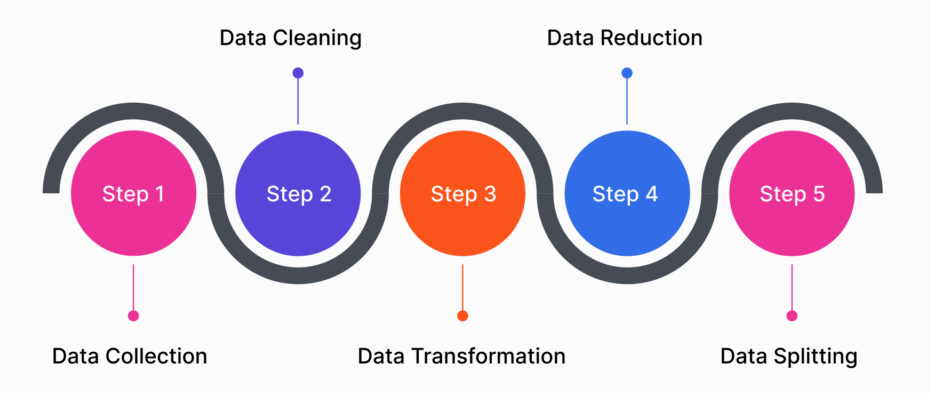
\includegraphics[scale=0.4]{figuras/steps_data_preparing.png}
	\end{center}
	\fonte{\cite{pecan_data_prep_2023}}
\end{figure}

\section{Coleta de dados}

Considerando a premissa do trabalho, em que a previsão do nível do rio será dada a partir de dados meteorológicos da cidade de Porto Alegre, junto aos dados de monitoramento do nível dos rios que constituem a bacia do Guaíba, duas fontes de dados foram utilizadas. Para os dados meteorológicos, o portal do \glsxtrfull{INMET}\footnote{\url{https://portal.inmet.gov.br/}} foi utilizado, onde foram coletadas as informações de temperatura, umidade relativa do ar, precipitação e velocidade do vento. Já os dados de monitoramento dos rios foram coletados na página do \glsxtrfull{SEMA-RS}\footnote{\url{https://www.saladesituacao.rs.gov.br/dados}} da internet (Sala de situação), onde foram coletados os dados de nível do rio Guaíba,Caí, Jacuí, Sinos e Gravataí. Os dados meteorológicos foram coletados em formato \glsxtrfull{CSV}, com arquivos separados por ano de monitoramento, com frequência horária. Os dados dos níveis dos rios foram coletados no formato \textit{.xlsx}, com histórico completo de amostragem das informações em frequência de 15 minutos, utilizando a biblioteca \textit{Pandas} do Python.

\section{Pré processamento dos dados}

Antes de seguir para a etapa de limpeza dos dados mostrado na Figura \ref{fig:passos_preparacao}, os dados coletados necessitam de um pré-processamento específico para cada uma das fontes utilizadas. Para os dados meteorológicos, devido às informações estarem separadas por ano de monitoramento, foi necessário concatenar os arquivos de cada ano em um único arquivo, utilizando a função \textit{concat} da biblioteca \textit{Pandas}, removendo o cabeçalho de informações geográficas da estação, ilustrado nas linhas 1 a 8 Figura \ref{fig:base_inmet}. Além disso, foi necessário combinar as duas primeiras colunas e converter o formato de data e hora para o padrão \textit{datetime}, utilizando a função \textit{to\_datetime} da mesma biblioteca. 

\begin{figure}[H]
	\caption{\label{fig:base_inmet}Dados meteorológicos.}
	\begin{center}
		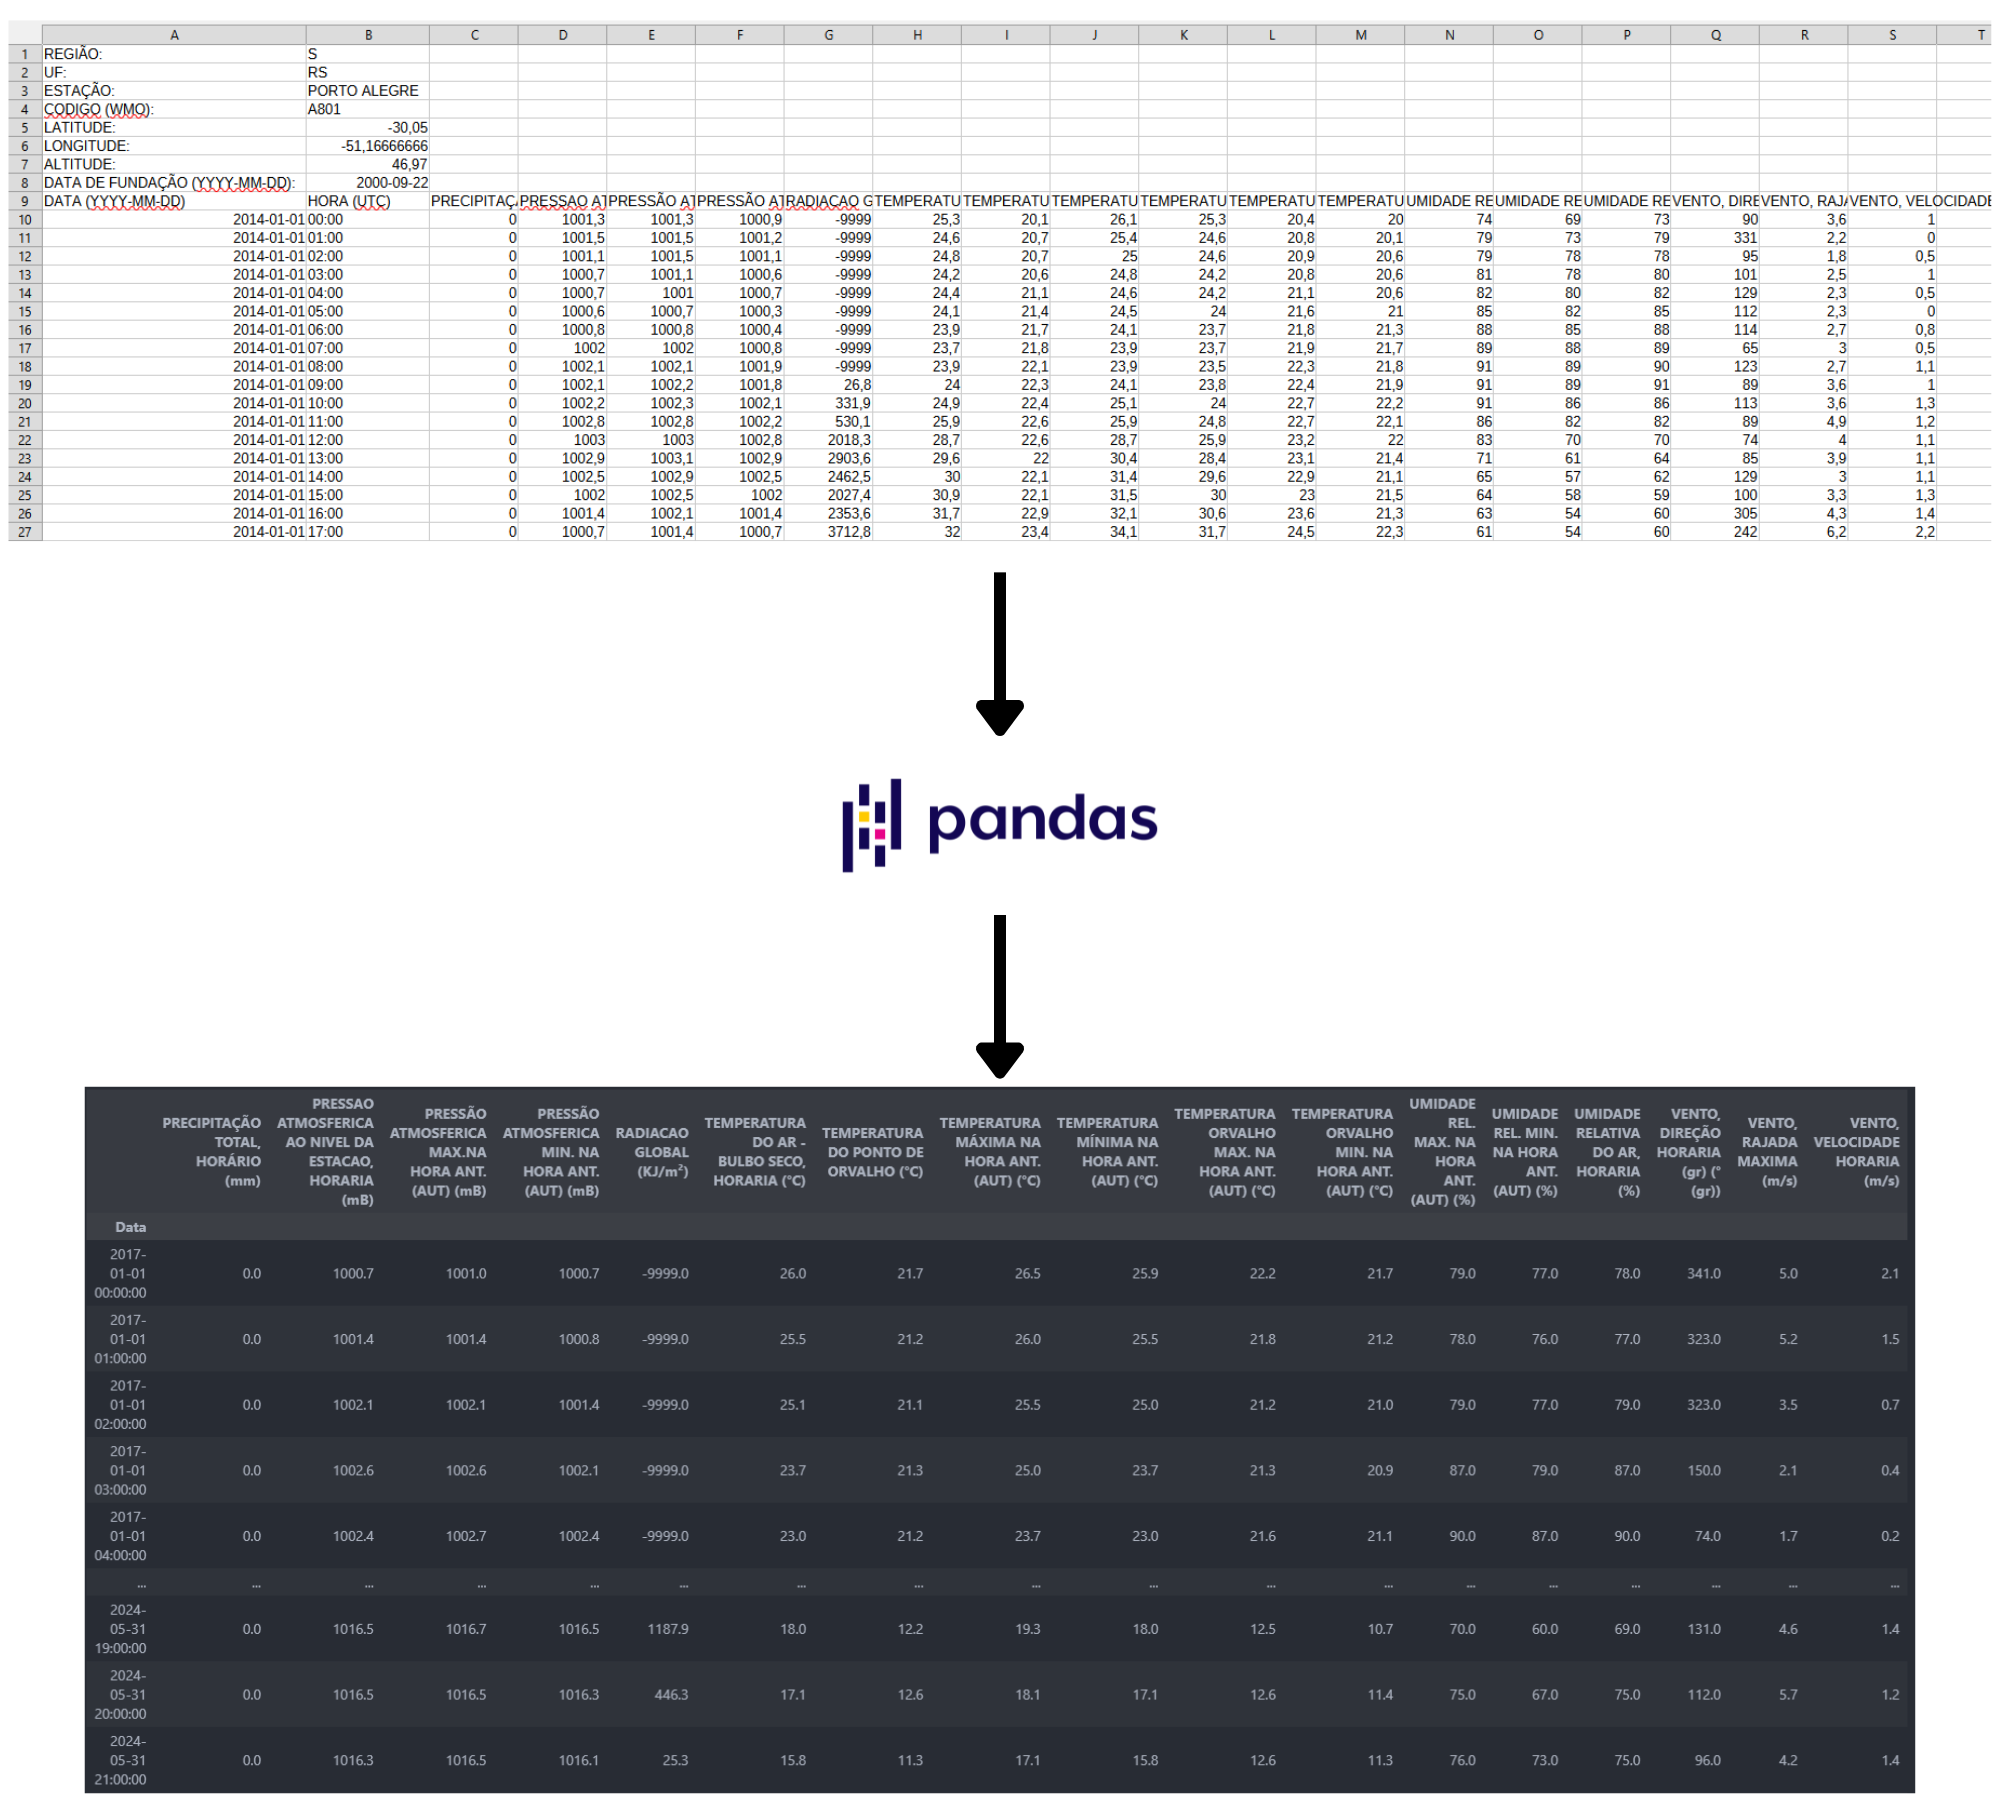
\includegraphics[scale=0.5]{figuras/base_inmet.png}
	\end{center}
	\fonte{Autor.}
\end{figure}

Analisando as colunas e os seus respectivos tipos de dados, tem-se a seguinte tabela:

\begin{table}[H]
	\centering
	\begin{tabular}{|p{10cm}|c|}
	\hline
	\textbf{Coluna} & \textbf{Tipo} \\
	\hline
	Precipitação Total (mm) & float64 \\
	Pressão Atmosférica ao Nível da Estação (mB) & float64 \\
	Pressão Atmosférica Máx. na Hora Anterior (mB) & float64 \\
	Pressão Atmosférica Mín. na Hora Anterior (mB) & float64 \\
	Radiação Global (kJ/m²) & float64 \\
	Temperatura do Ar - Bulbo Seco (°C) & float64 \\
	Temperatura do Ponto de Orvalho (°C) & float64 \\
	Temperatura Máxima na Hora Anterior (°C) & float64 \\
	Temperatura Mínima na Hora Anterior (°C) & float64 \\
	Temperatura Orvalho Máx. na Hora Anterior (°C) & float64 \\
	Temperatura Orvalho Mín. na Hora Anterior (°C) & float64 \\
	Umidade Relativa Máx. na Hora Anterior (\%) & float64 \\
	Umidade Relativa Mín. na Hora Anterior (\%) & float64 \\
	Umidade Relativa do Ar (\%) & float64 \\
	Vento - Direção Horária (° (gr)) & float64 \\
	Vento - Rajada Máxima (m/s) & float64 \\
	Vento - Velocidade Horária (m/s) & float64 \\
	\hline
	\end{tabular}
	\caption{Tabela de tipos de dados da base de informações meteorológicas.}
	\label{tab:colunas_dados_meteorologicos}
\end{table}

Para os dados dos níveis dos rios, também foi necessário remover o cabeçalho com dados geográficos da estação de monitoramento, como mostra a Figura \ref{fig:base_sema}, junto da conversão do formato de data e hora para o padrão \textit{datetime} da primeira coluna.

\begin{figure}[H]
	\caption{\label{fig:base_sema}Dados do nível do rio.}
	\begin{center}
		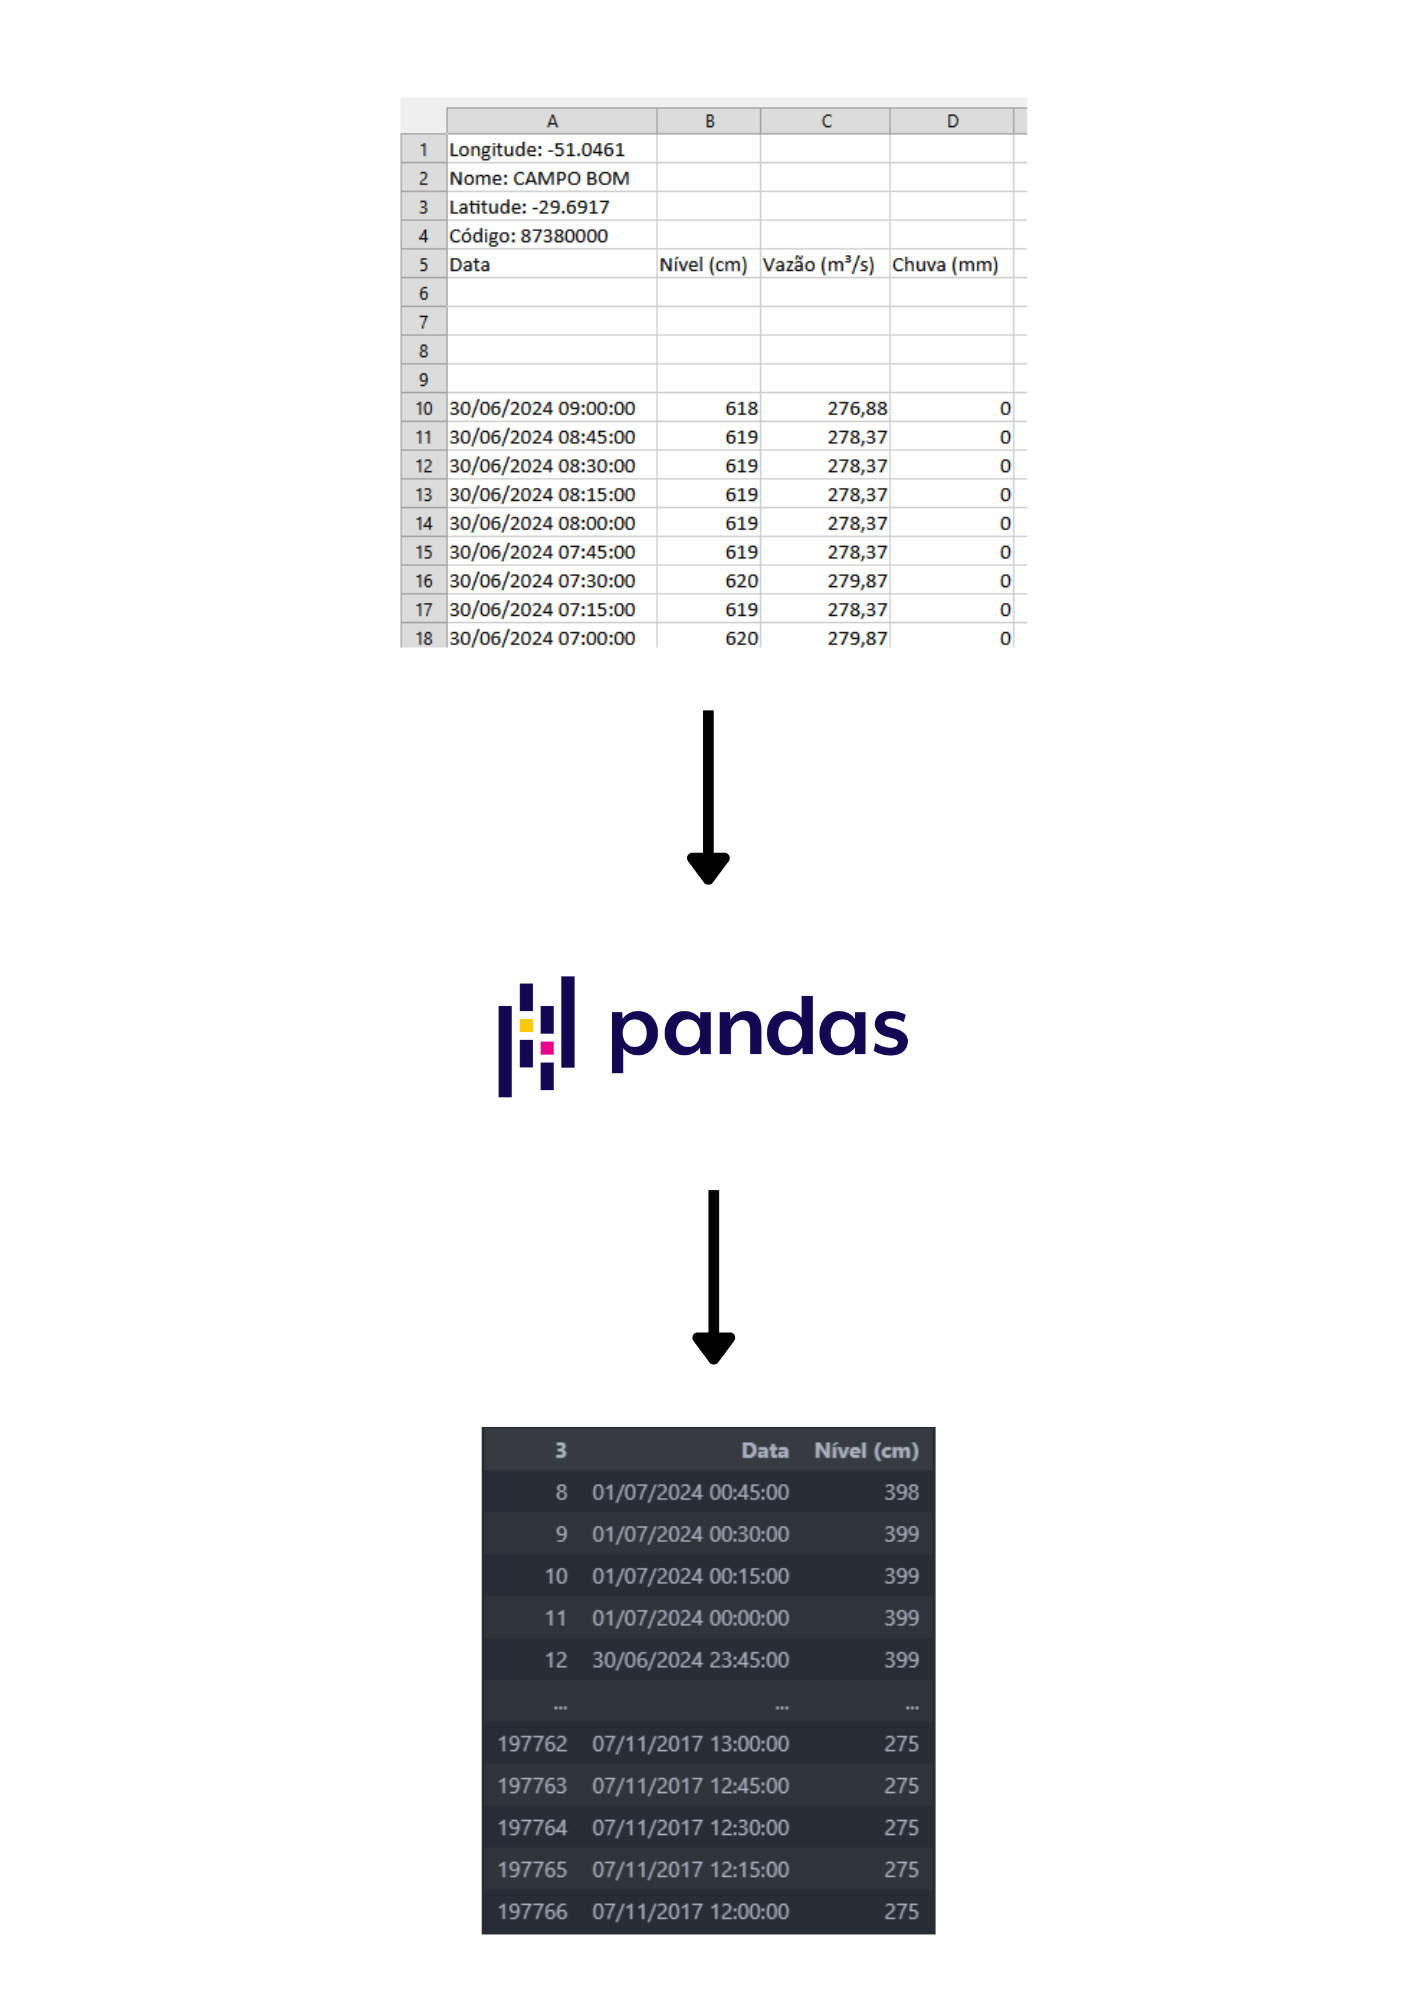
\includegraphics[scale=0.5]{figuras/base_sema.png}
	\end{center}
	\fonte{Autor.}
\end{figure}

\section{Limpeza dos dados}
\label{sec:limpeza_dos_dados}

Após a coleta dos dados, o próximo passo é a limpeza dessas informações, cujo procedimento consiste em remover dados duplicados, corrigir erros de formatação e lidar com valores ausentes. Existem diferentes abordagens para tratar valores inconsistentes no dados coletados. Uma abordagem comum, principalmente em casos onde não há uma linearidade ou tendência clara é o preenchimento com zero \cite{cousineau2010outliers}, como mostra a Figura \ref{fig:passo_dados_limpeza}, ou com a média dos dados na coluna a ser limpa.

\begin{figure}[H]
	\caption{\label{fig:passo_dados_limpeza}Limpeza dos dados coletados.}
	\begin{center}
		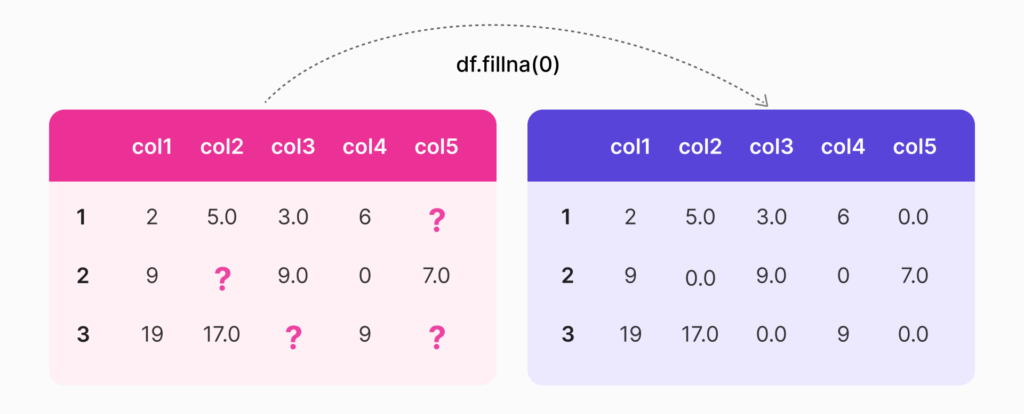
\includegraphics[scale=0.4]{figuras/step_data_cleaning.png}
	\end{center}
	\fonte{\cite{pecan_data_prep_2023}}
\end{figure}

Nessa etapa, na base de dados meteorológicos, optou-se por preencher os dados ausentes, representados por ''-'', e os dados com valor igual a ''-9999'' por zero, já que dados meteorológicos tendem a ser mais voláteis e não apresentam uma tendência clara. Desse modo, a abordagem de aproximação linear é descartada, a fim de não comprometer a análise do modelo de previsão.  

Tomando como exemplo a coluna \textit{TEMPERATURA ORVALHO MAX. NA HORA ANT. (AUT) (°C)}, na Figura \ref{fig:dados_clima_poa_nao_tratados}, observa-se os valores ausentes representados por ''-'' e ''-9999'', evidenciados na Figura pelos pontos distantes do restante dos dados.

\begin{figure}[H]
	\caption{\label{fig:dados_clima_poa_nao_tratados}Gráfico de Temperatura do orvalho Máx. na Hora Anterior (°C) não tratado.}
	\begin{center}
		\includegraphics[scale=0.35]{figuras/TEMPERATURA ORVALHO MAX. NA HORA ANT. (AUT) (°C) SEM TRATAMENTO_edit.png}
	\end{center}
	\fonte{Autor.}
\end{figure}

Após a substituição dos valores ausentes por zero, o gráfico da mesma coluna, mostrado na Figura \ref{fig:dados_clima_poa_tratados}, apresenta uma distribuição mais uniforme, sem os picos de dados ausentes.

\begin{figure}[H]
	\caption{\label{fig:dados_clima_poa_tratados}Gráfico de Temperatura do orvalho Máx. na Hora Anterior (°C) tratado.}
	\begin{center}
		\includegraphics[scale=0.35]{figuras/TEMPERATURA ORVALHO MAX. NA HORA ANT. (AUT) (°C) COM TRATAMENTO.png}
	\end{center}
	\fonte{Autor.}
\end{figure}

Aplicado o tratamento, a coluna \textit{TEMPERATURA ORVALHO MAX. NA HORA ANT. (AUT) (°C)} passa a apresentar uma distribuição mais uniforme, sem os picos de dados ausentes, com valores condizentes com a escala esperada da unidade medida, neste caso, a temperatura em graus Celsius.

Em casos onde os dados apresentam \textit{outliers} (dados que se distanciam significativamente do restante da coluna analisada), foi aplicado o método \glsxtrfull{IQR} para identificar e remover esses valores. A partir da diferença entre o terceiro quartil (Q3) e o primeiro quartil (Q1) de um conjunto de dados, multiplicado por um fator de tolerância, o método determina limites superiores e inferiores para o conjunto de dados analisado, removendo ou substituindo os valores que estão fora dessa faixa, para manter a consistência das informações.

Por exemplo, na coluna \textit{UMIDADE REL. MAX. NA HORA ANT. (AUT) (\%)}, as Figuras \ref{fig:dados_outlier_sem_tratamento} e \ref{fig:dados_outlier_com_tratamento} mostram a diferença entre os dados após a aplicação do método \gls{IQR}, com um fator de tolerância de 1.2 entre os interquartis Q1 e Q3.

\begin{figure}[H]
	\caption{\label{fig:dados_outlier_sem_tratamento}Gráfico de Umidade Relativa Máxima  na Hora Anterior (\%) sem tratamento.}
	\begin{center}
		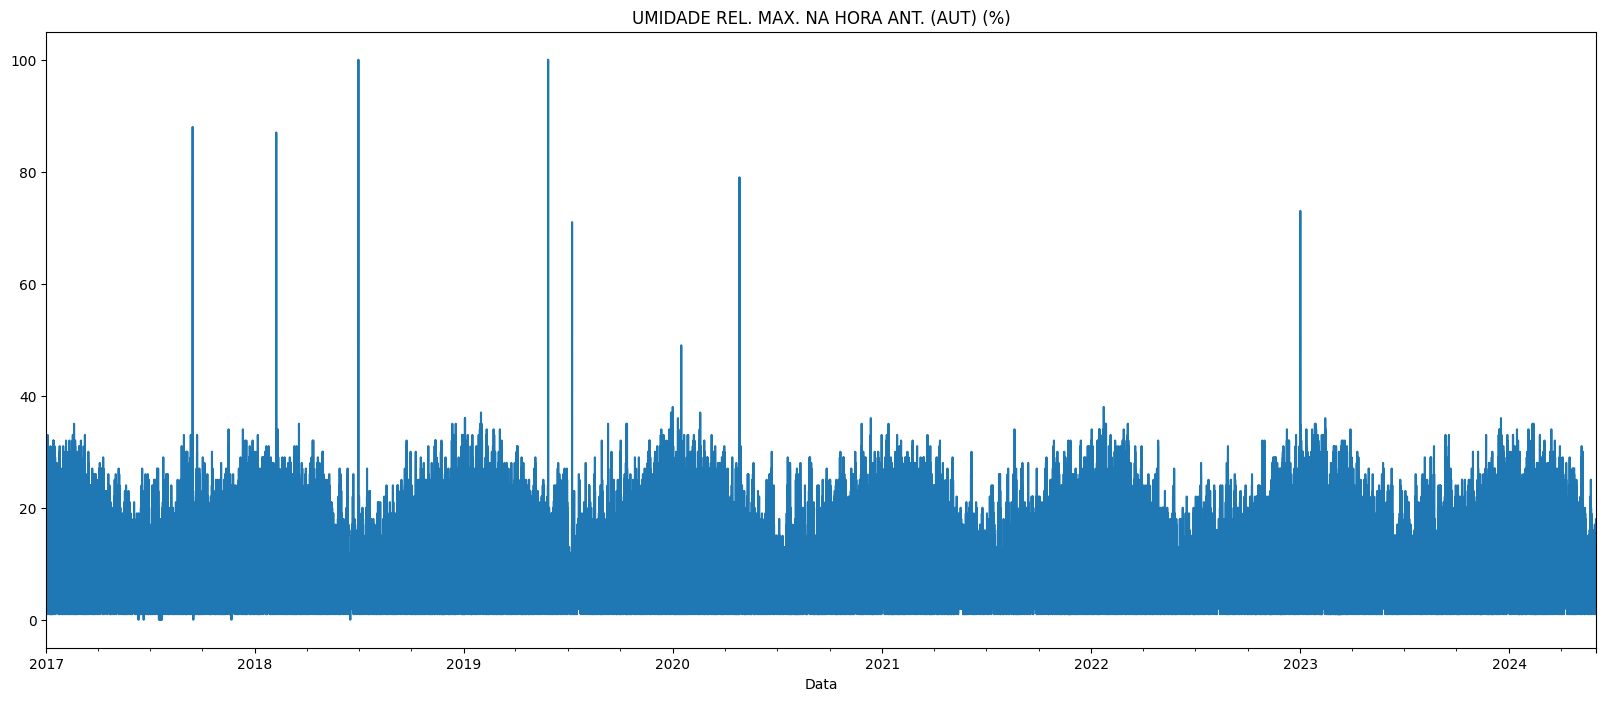
\includegraphics[scale=0.35]{figuras/UMIDADE REL. MAX. NA HORA ANT. (AUT) SEM TRATAMENTO.png}
	\end{center}
	\fonte{Autor.}
\end{figure}

\begin{figure}[H]
	\caption{\label{fig:dados_outlier_com_tratamento}Gráfico de Umidade Relativa Máxima  na Hora Anterior (\%) com tratamento.}
	\begin{center}
		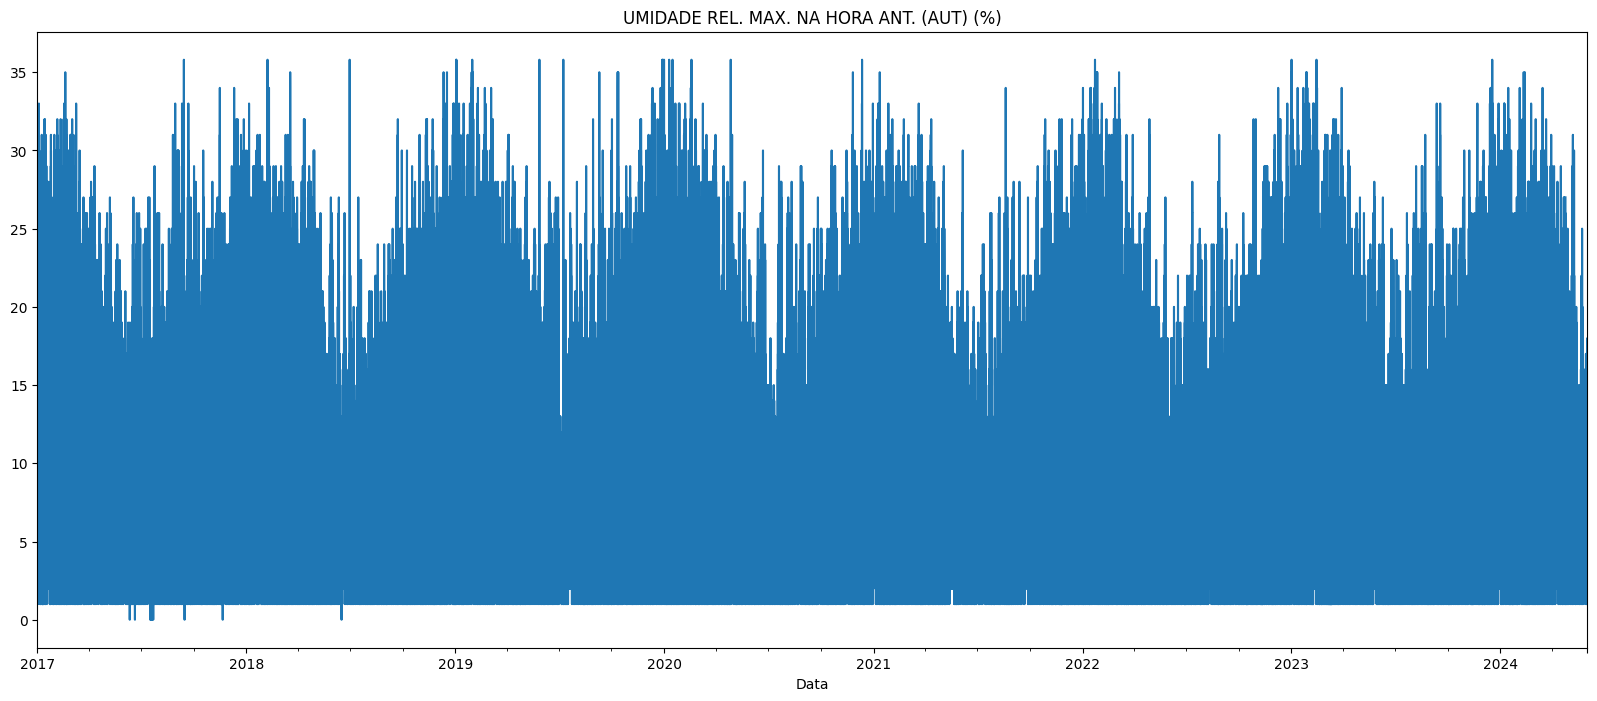
\includegraphics[scale=0.35]{figuras/UMIDADE REL. MAX. NA HORA ANT. (AUT) COM TRATAMENTO.png}
	\end{center}
	\fonte{Autor.}
\end{figure}

Na base de dados dos níveis dos rios, embora a dinâmica que representa os respectivos comportamentos não seja linear, o uso do conceito de aproximação linear permite preencher os dados ausentes por meio da interpolação entre os valores que cercam as células sem informação em determinado período. Essa abordagem é válida, uma vez que a variação do nível do rio entre dois pontos de amostragem próximos tende a ser linear, já que o nível do rio não apresenta oscilações bruscas em curtos períodos de tempo.

Para realizar a interpolação, utilizou-se a função \textit{interpolate} com o argumento \textit{method = linear} da biblioteca \textit{Pandas}, que preenche os valores ausentes com base nos dados adjacentes.

Ainda, observou-se nas bases dos níveis dos rios a ocorrência de valores ausentes no início ou no final do período de amostragem, inviabilizando a interpolação. Para esses casos, o preenchimento foi feito a partir da repetição do primeiro ou do último valor disponível, respectivamente. É importante ressaltar que tal limpeza só pode ser feita se o preenchimento ocorra em um intervalo de tempo curto, visando não afetar a análise feita pelo modelo de previsão.

\section{Redução dos dados}

A etapa de redução dos dados visa eliminar informações redundantes ou irrelevantes, mantendo apenas os dados que contribuem para a análise e treinamento do modelo de previsão. Considerando que serão utilizados dados de monitoramento do nível de 4 rios para a previsão do nível do rio Guaíba, os dados meteorológicos coletados precisam ser filtrados de modo a garantir tanto que as informações sejam relevantes para a previsão, quanto que os dados de monitoramento dos rios estejam alinhados com os dados meteorológicos, evitando assim a inclusão de dados desnecessários no treinamento. 

Voltando para a Tabela \ref{tab:colunas_dados_meteorologicos}, nota-se a presença de 17 colunas, das quais:

\begin{itemize}
	\item 6 colunas referem-se a dados de temperatura;
	\item 3 colunas referem-se a dados de pressão atmosférica;
	\item 3 colunas referem-se a dados do comportamento do vento;
	\item 3 colunas referem-se a dados de umidade relativa do ar;
	\item 1 coluna refere-se a dados de radiação solar.
	\item 1 coluna refere-se a dados de precipitação.
\end{itemize}

Desse modo, para o primeiro passo de redução da base, foram mantidas apenas uma coluna de cade tipo de medição meteorológica, filtrando 6 colunas no total, conforme a Tabela \ref{tab:colunas_dados_meteorologicos_reduzidas}. 

\begin{table}[H]
	\centering
	\begin{tabular}{|p{10cm}|c|}
	\hline
	\textbf{Coluna} & \textbf{Unidade de medida} \\
	\hline
	Temperatura do Ar - Bulbo seco & (°C) \\
	Pressão Atmosférica ao Nível da Estação & (mB) \\
	Vento - Velocidade Horária & (m/s) \\
	Umidade Relativa do Ar & (\%) \\
	Radiação Global & (kJ/m²) \\
	Precipitação Total & (mm) \\
	\hline
	\end{tabular}
	\caption{Tabela de dados meteorológicos reduzidos - 1ª Filtragem}
	\label{tab:colunas_dados_meteorologicos_reduzidas}
\end{table}

Para a escolha das colunas a serem mantidas, foram levados em consideração os seguintes critérios:
\begin{itemize}
	\item As colunas \textit{Temperatura do Ar - Bulbo seco}, \textit{Pressão Atmosférica ao Nível da Estação} e \textit{Umidade Relativa do Ar} foram escolhidas por serem medidas diretas dos respectivos fenômenos atmosféricos, enquanto as demais colunas referem-se a medidas derivadas ou não diretamente observáveis, que não são tão relevantes para a previsão do nível do rio. Além disso, observou-se que para essas unidades de medida derivadas, o comportamento dos dados eram semalhantes, descartanto a necessidade de manter mais de uma coluna para cada tipo de medição, como mostra a Figura \ref{fig:comparacao_temp} em relação às medidas de temperatura.
	\begin{figure}[H]
	\caption{\label{fig:comparacao_temp}Comparativo de gráficos de temperatura em diferentes tipos de medição}
	\begin{center}
		\begin{subfigure}{0.35\textwidth}
			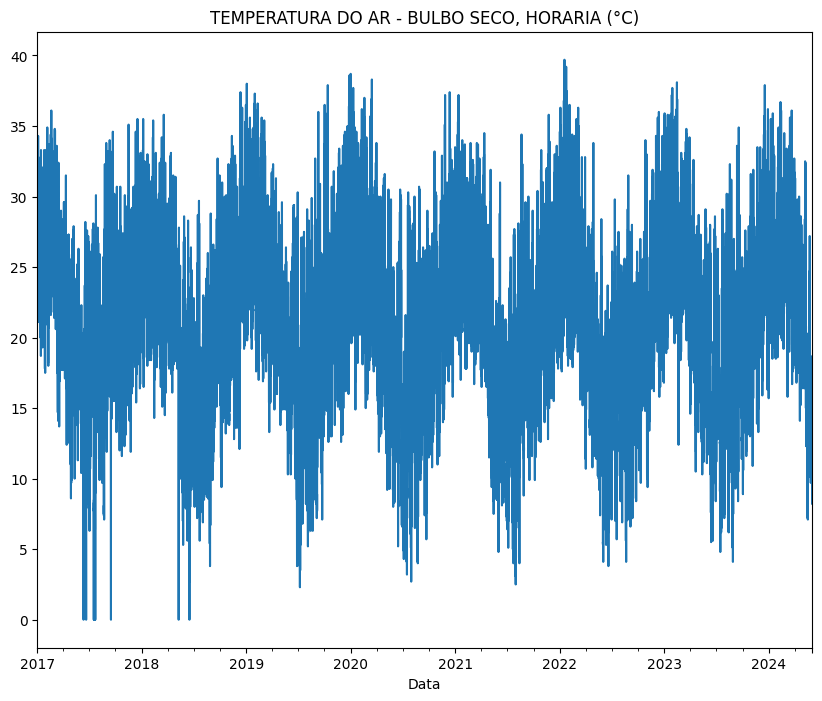
\includegraphics[width=\linewidth]{figuras/comparacao_temp_1.png}
		\end{subfigure}
		\begin{subfigure}{0.35\textwidth}
			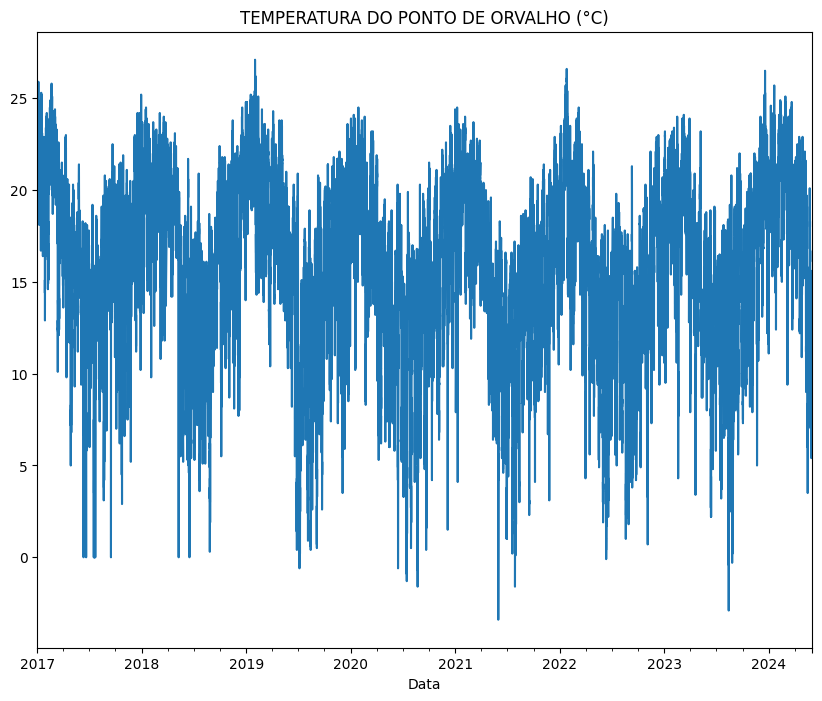
\includegraphics[width=\linewidth]{figuras/comparacao_temp_2.png}
		\end{subfigure}
		
		\begin{subfigure}{0.35\textwidth}
			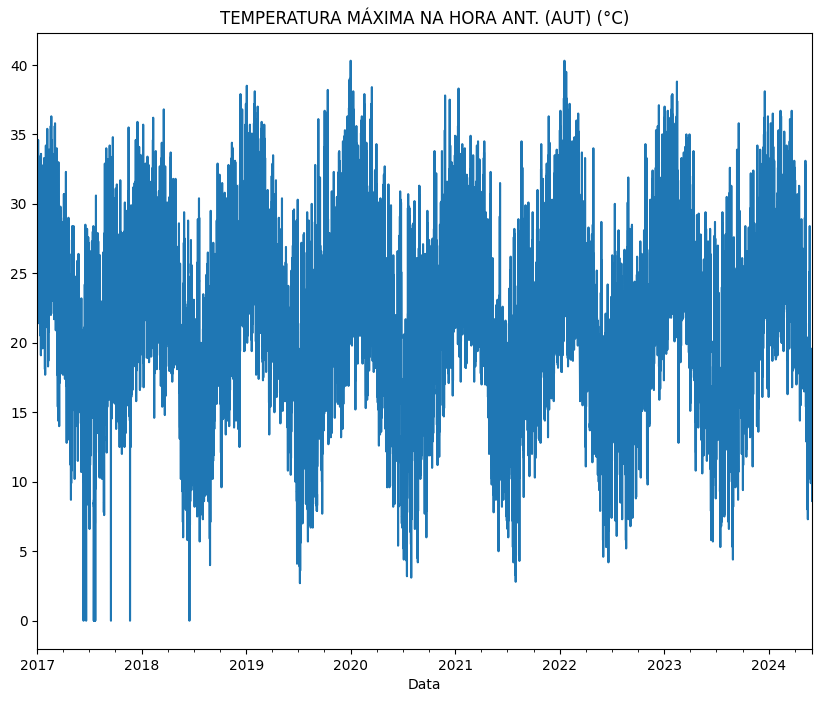
\includegraphics[width=\linewidth]{figuras/comparacao_temp_3.png}
		\end{subfigure}
		\begin{subfigure}{0.35\textwidth}
			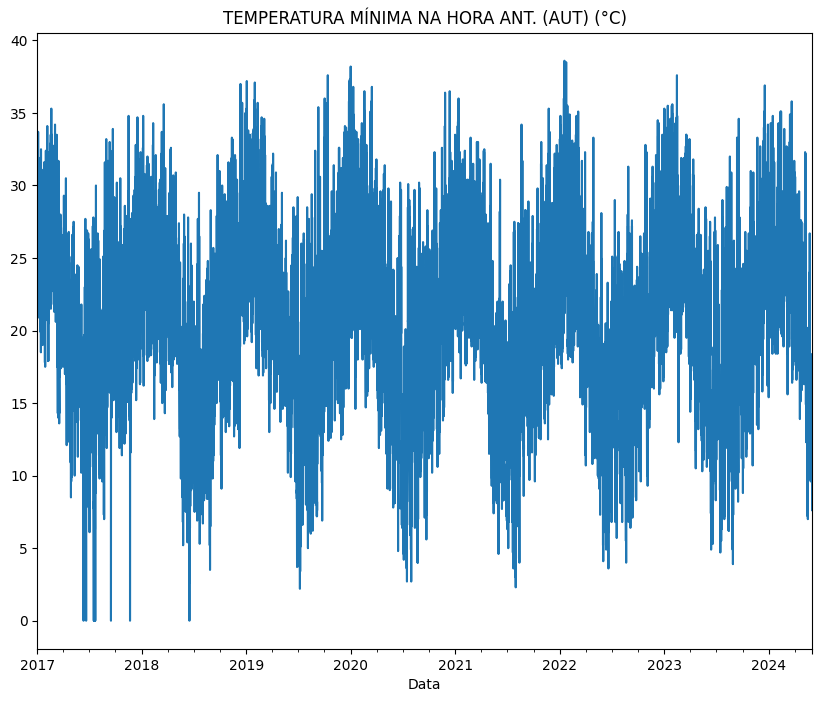
\includegraphics[width=\linewidth]{figuras/comparacao_temp_4.png}
		\end{subfigure}
		
		\begin{subfigure}{0.35\textwidth}
			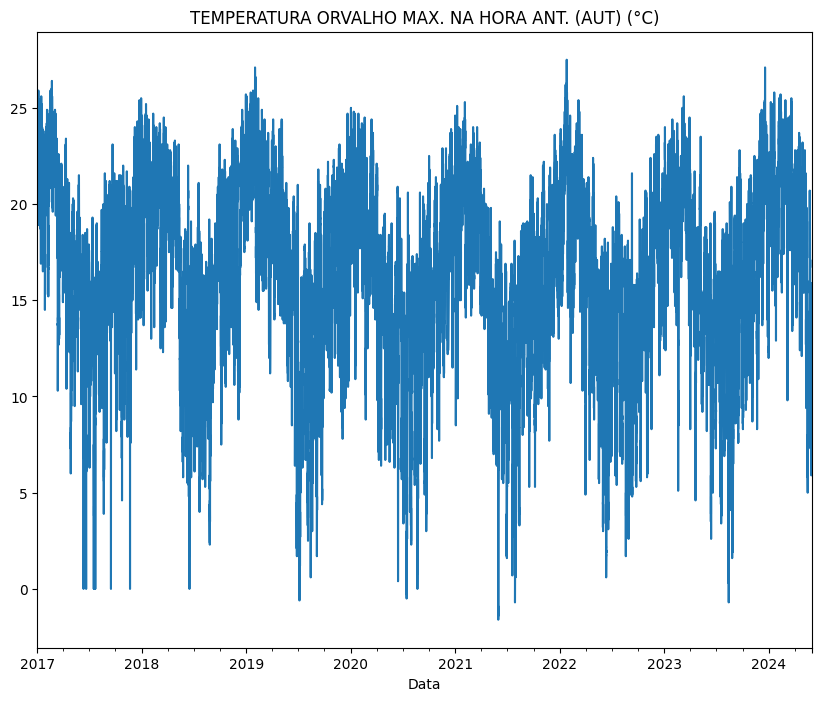
\includegraphics[width=\linewidth]{figuras/comparacao_temp_5.png}
		\end{subfigure}
		\begin{subfigure}{0.35\textwidth}
			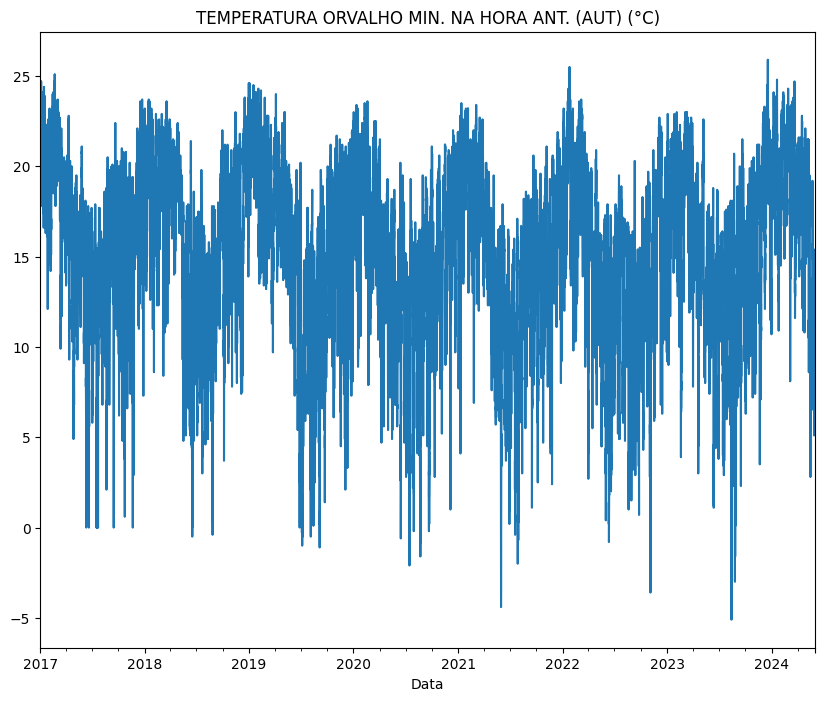
\includegraphics[width=\linewidth]{figuras/comparacao_temp_6.png}
		\end{subfigure}
	\end{center}
	\fonte{Autor.}
	\end{figure}
	\item A coluna \textit{Precipitação Total} foi mantida por ser um dos principais fatores que influenciam o nível do rio.
	\item As colunas \textit{Radiação Global} e \textit{Umidade Relativa do Ar} foram mantidas por serem fatores importantes para a evaporação da água, que também influenciam, mesmo que de forma indireta, no nível do rio.
\end{itemize}

Após essa redução inicial, os gráficos e seus dados de cada coluna foram analisados, a fim de verificar se as informações eram consistentes e poderiam contribuir para o treinamento do modelo. Nas Figuras \ref{fig:temperatura_do_ar_bulbo_seco}, \ref{fig:pressao_atmosferica_ao_nivel_da_estacao}, \ref{fig:vento_velocidade_horaria}, \ref{fig:umidade_relativa_do_ar}, \ref{fig:radiacao_global} e \ref{fig:precipitacao_total}, são apresentados os gráficos de cada uma das colunas mantidas.

\begin{figure}[H]
	\caption{\label{fig:temperatura_do_ar_bulbo_seco}Gráfico de Temperatura do Ar - Bulbo Seco}
	\begin{center}
		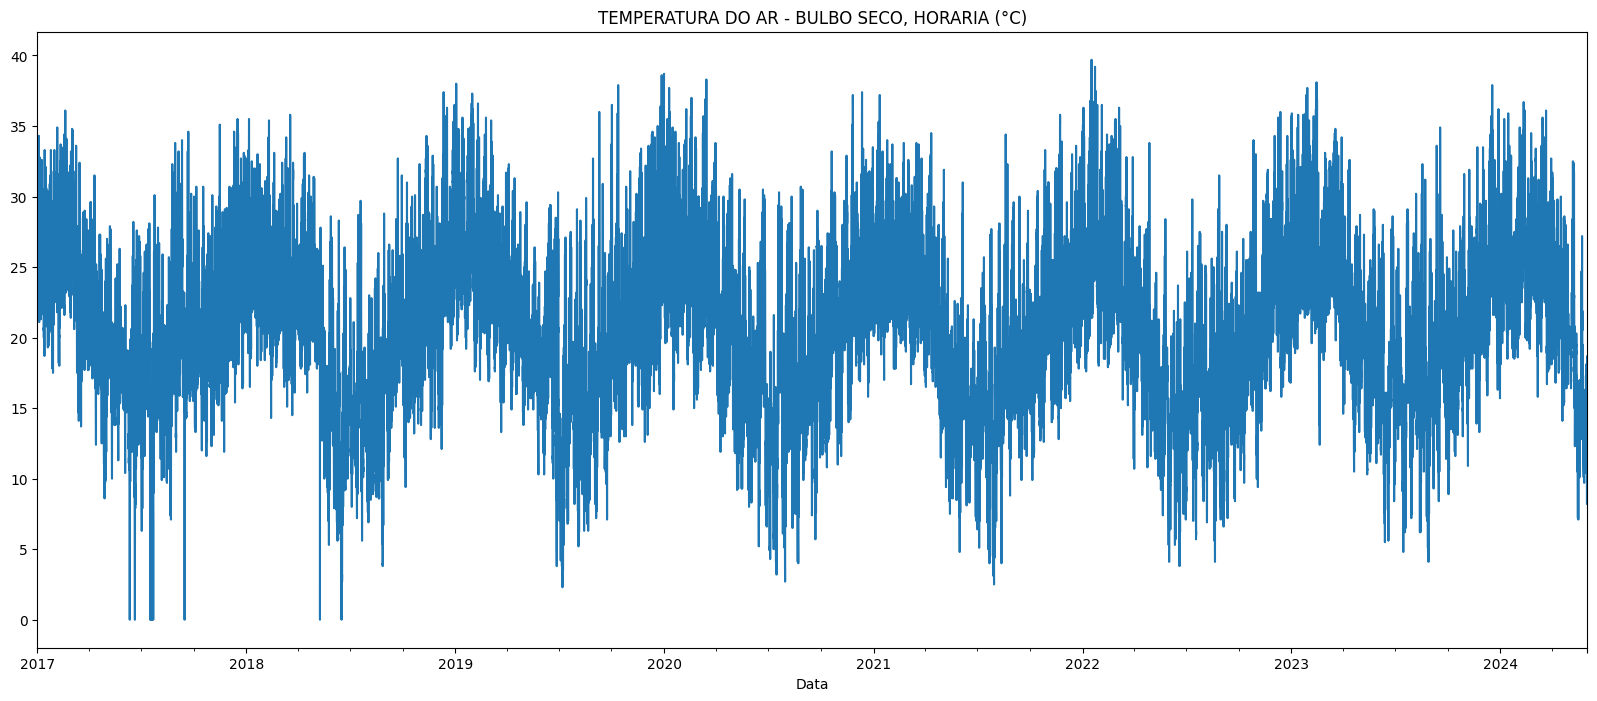
\includegraphics[scale=0.35]{figuras/temperatura_do_ar_bulbo_seco.png}
	\end{center}
	\fonte{Autor.}
\end{figure}

\begin{figure}[H]
	\caption{\label{fig:pressao_atmosferica_ao_nivel_da_estacao}Gráfico de Pressão Atmosférica ao Nível da Estação.}
	\begin{center}
		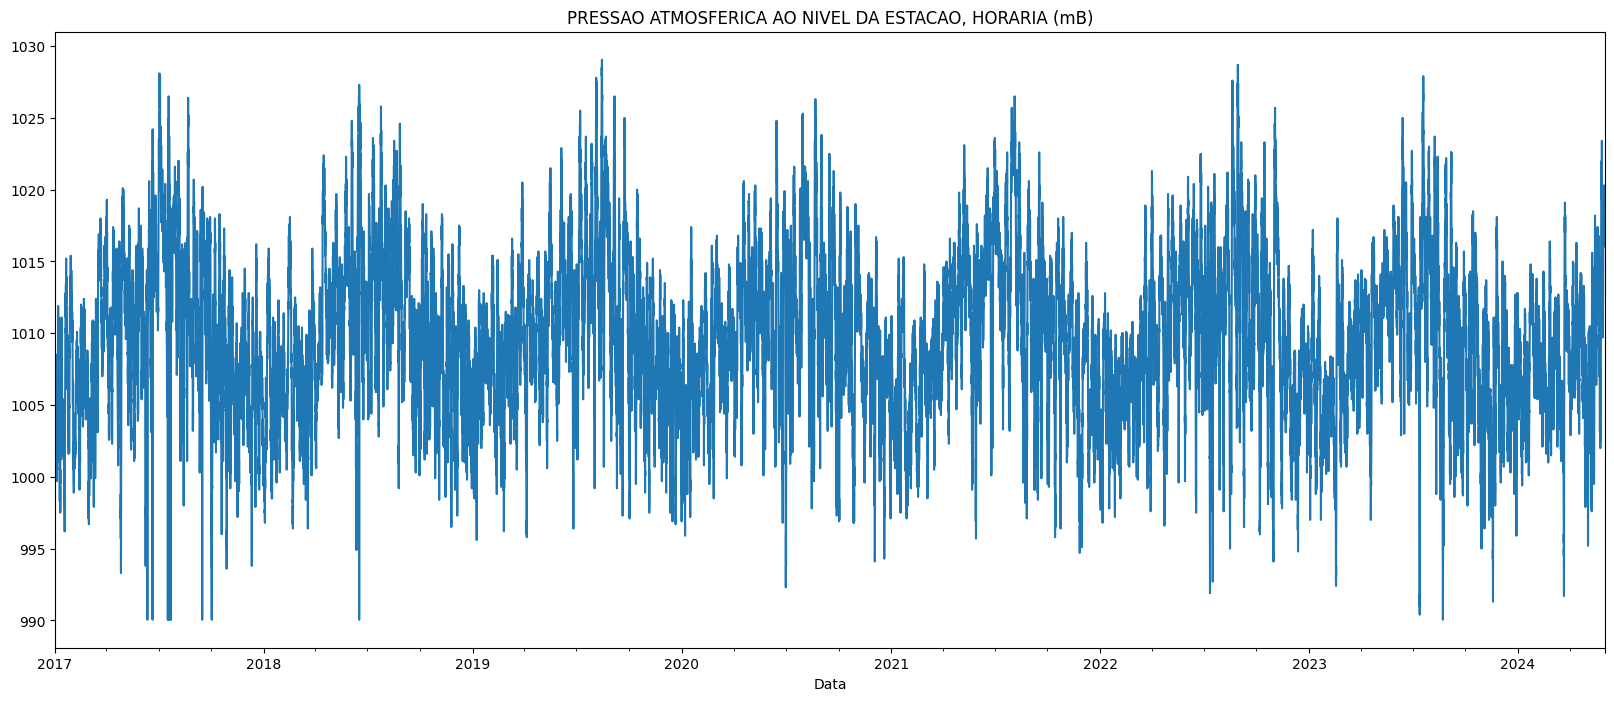
\includegraphics[scale=0.35]{figuras/pressao_atmosferica_ao_nivel_da_estacao.png}
	\end{center}
	\fonte{Autor.}
\end{figure}

\begin{figure}[H]
	\caption{\label{fig:vento_velocidade_horaria}Gráfico de Vento - Velocidade Horária.}
	\begin{center}
		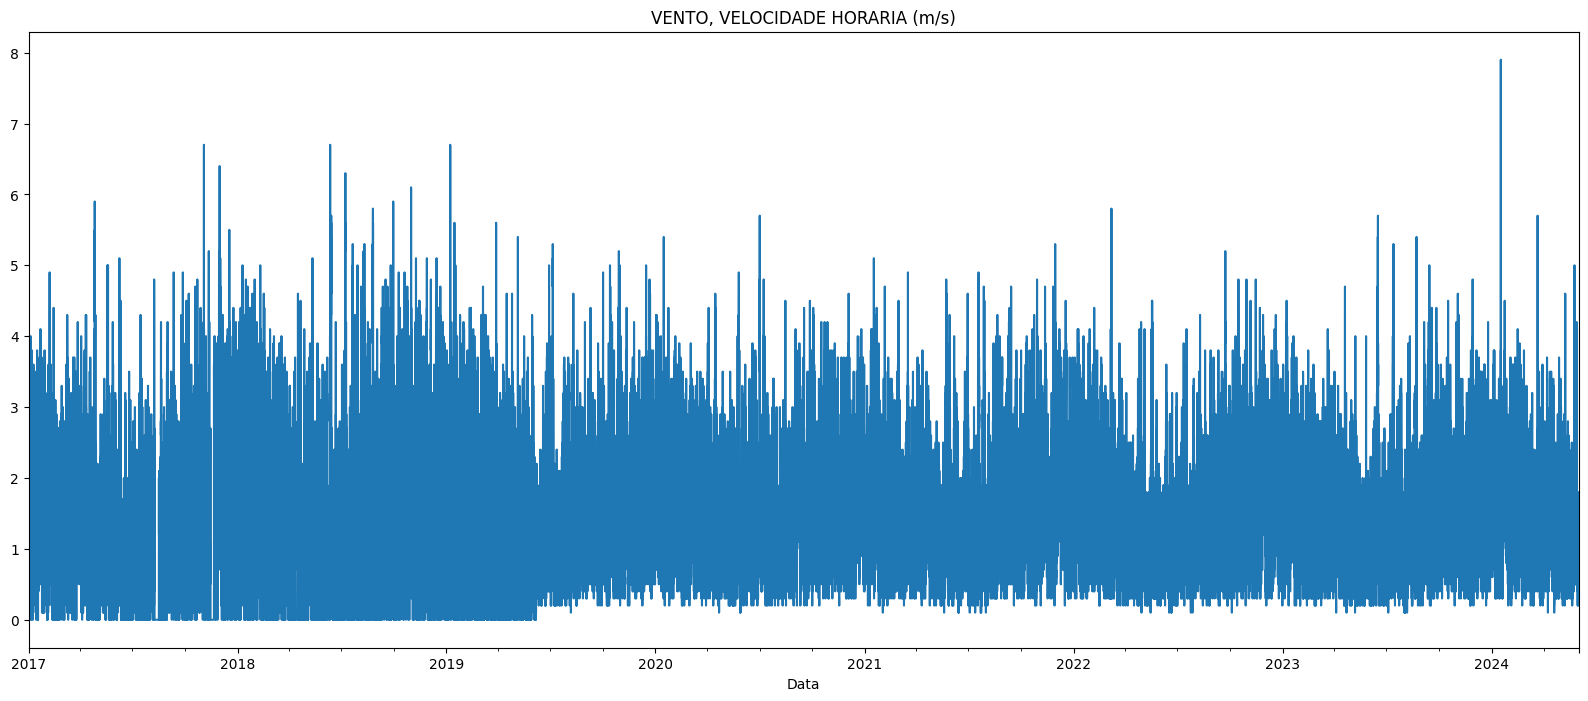
\includegraphics[scale=0.35]{figuras/vento_velocidade_horaria.png}
	\end{center}
	\fonte{Autor.}
\end{figure}

\begin{figure}[H]
	\caption{\label{fig:umidade_relativa_do_ar}Gráfico de Umidade Relativa do Ar}
	\begin{center}
		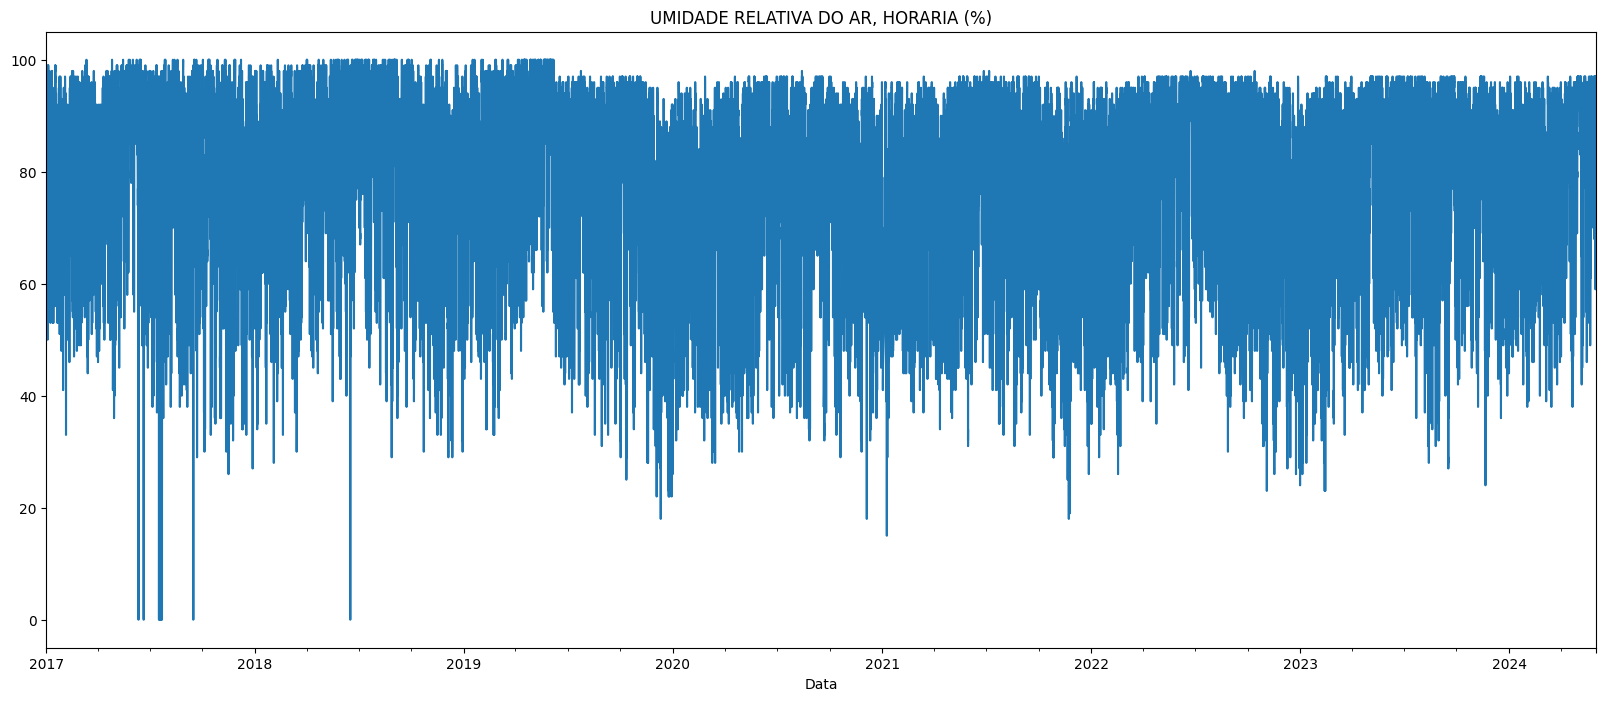
\includegraphics[scale=0.35]{figuras/umidade_relativa_do_ar.png}
	\end{center}
	\fonte{Autor.}
\end{figure}

\begin{figure}[H]
	\caption{\label{fig:radiacao_global}Gráfico de Radiação Global}
	\begin{center}
		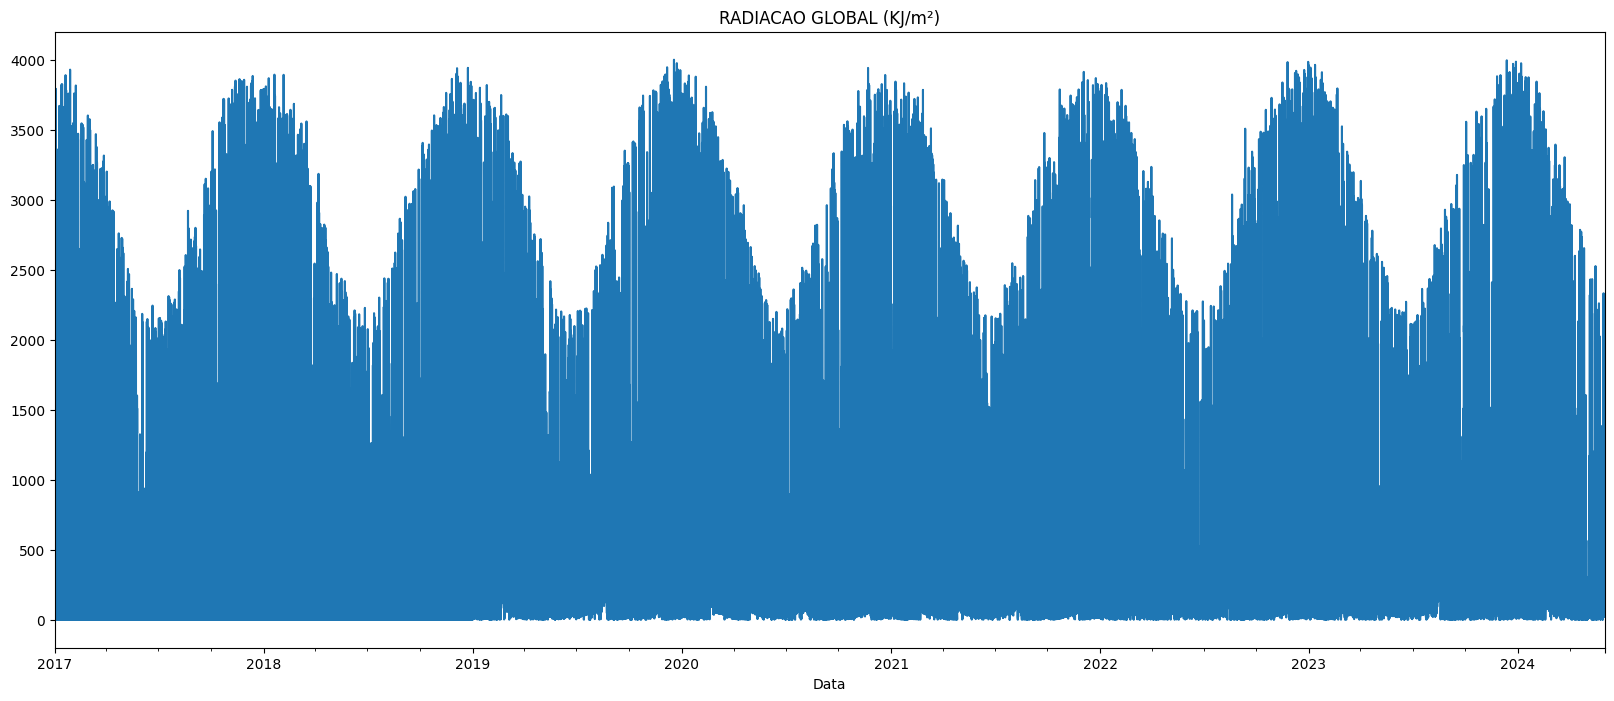
\includegraphics[scale=0.35]{figuras/radiacao_global.png}
	\end{center}
	\fonte{Autor.}
\end{figure}

\begin{figure}[H]
	\caption{\label{fig:precipitacao_total}Gráfico de Precipitação Total}
	\begin{center}
		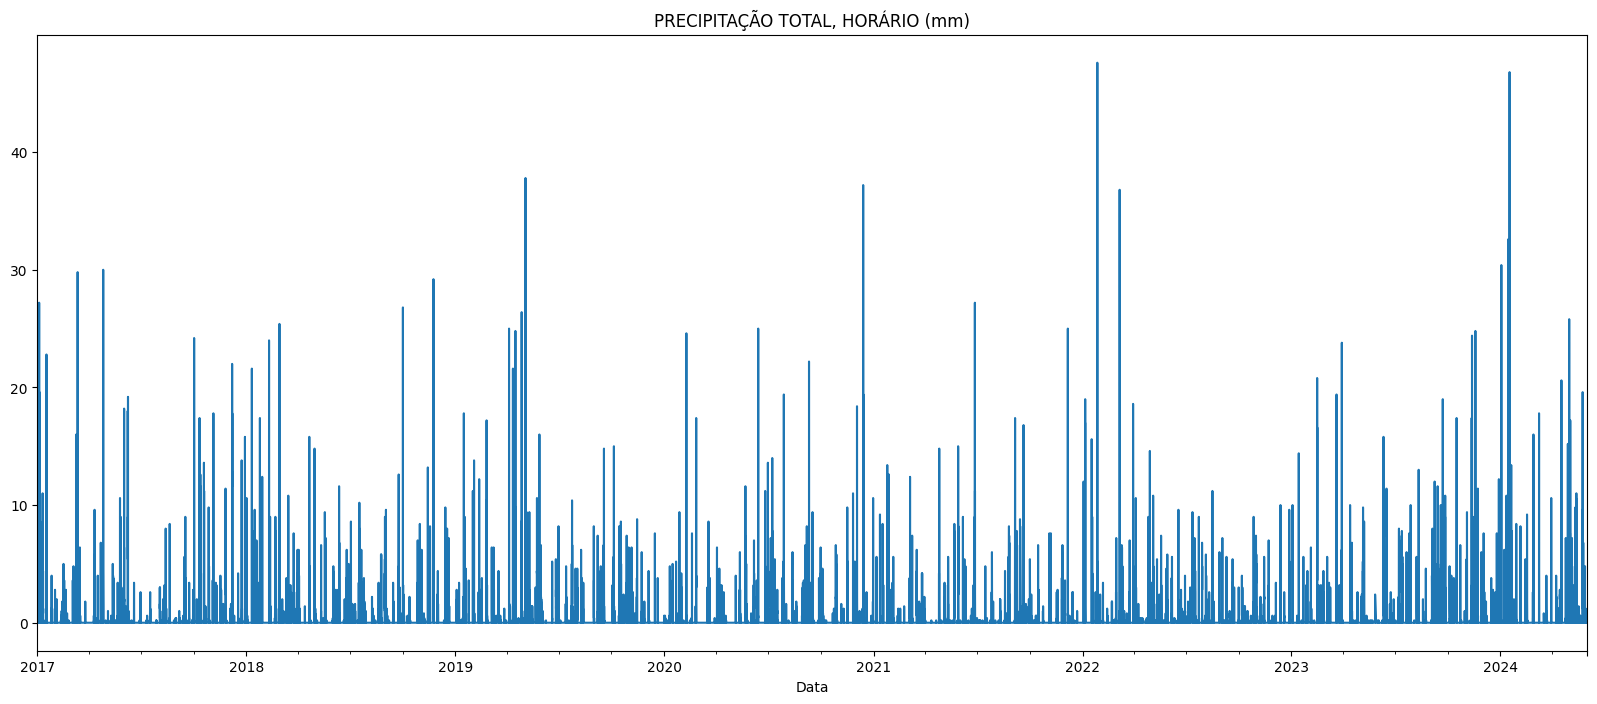
\includegraphics[scale=0.35]{figuras/precipitacao_total_horario.png}
	\end{center}
	\fonte{Autor.}
\end{figure}

As Figuras \ref{fig:temperatura_do_ar_bulbo_seco}, \ref{fig:pressao_atmosferica_ao_nivel_da_estacao} e \ref{fig:radiacao_global} ilustram um padrão sazonal nos dados, com aumentos e diminuições periódicas dos valores ao longo do ano, indicando uma correlação entre as variáveis meteorológicas e as estações do ano. Desse modo, torna-se justificável a manutenção dessas colunas, uma vez que o modelo de previsão pode se beneficiar dessa sazonalidade para melhorar a acurácia das previsões, considerando que o nível do rio também apresenta a mesma dinâmica, ilustrado nas Figura \ref{fig:comparacao_temp_nivel_rio}, \ref{fig:comparacao_pressao_nivel_rio} e \ref{fig:comparacao_radiacao_nivel_rio}.

\begin{figure}[H]
	\caption{\label{fig:comparacao_temp_nivel_rio}Gráfico comparativo de temperatura e nível quanto a sazonalidade}
	\begin{center}
		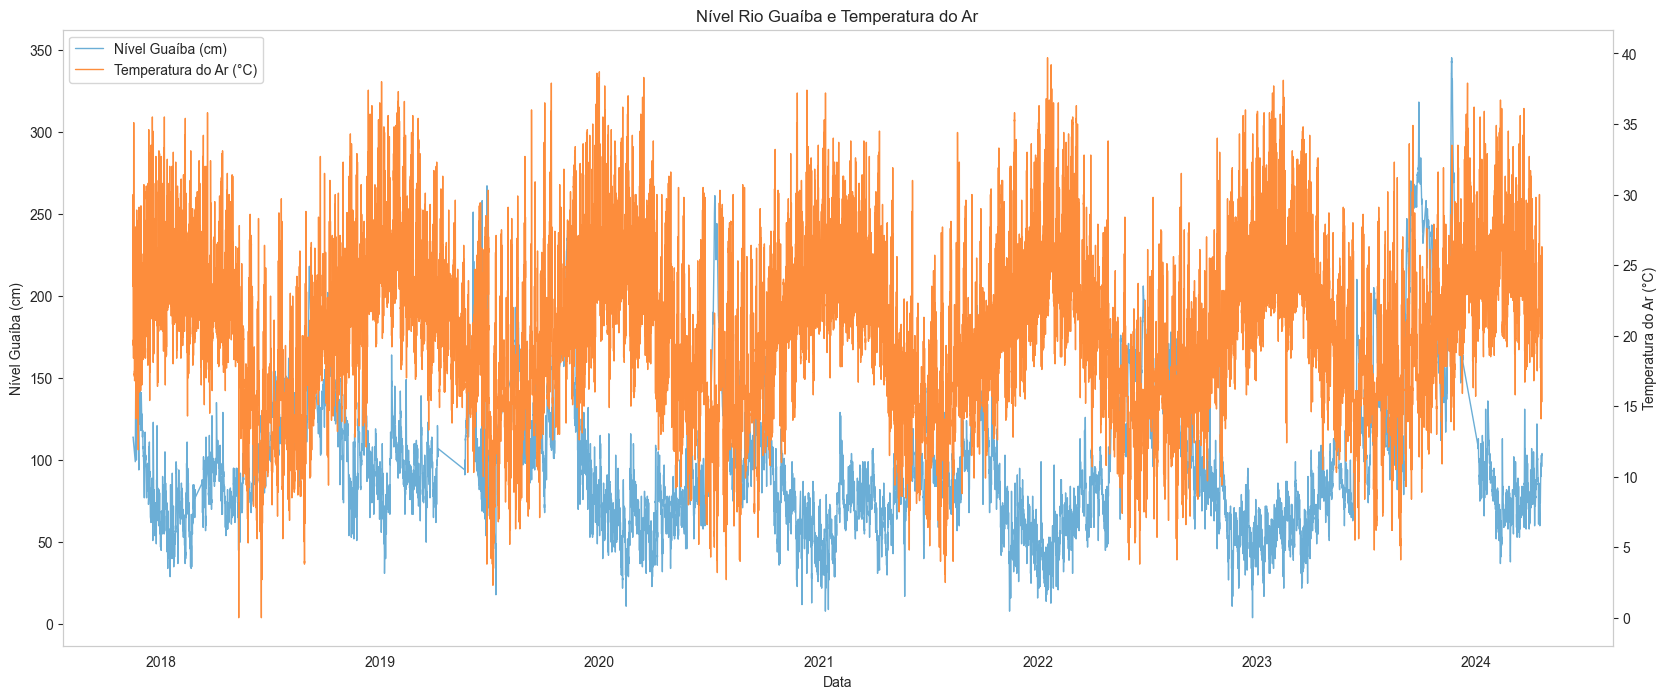
\includegraphics[scale=0.35]{figuras/comparacao_temp_nivel_rio.png}
	\end{center}
	\fonte{Autor.}
\end{figure}

\begin{figure}[H]
	\caption{\label{fig:comparacao_pressao_nivel_rio}Gráfico comparativo de pressão atmosférica e nível quanto a sazonalidade}
	\begin{center}
		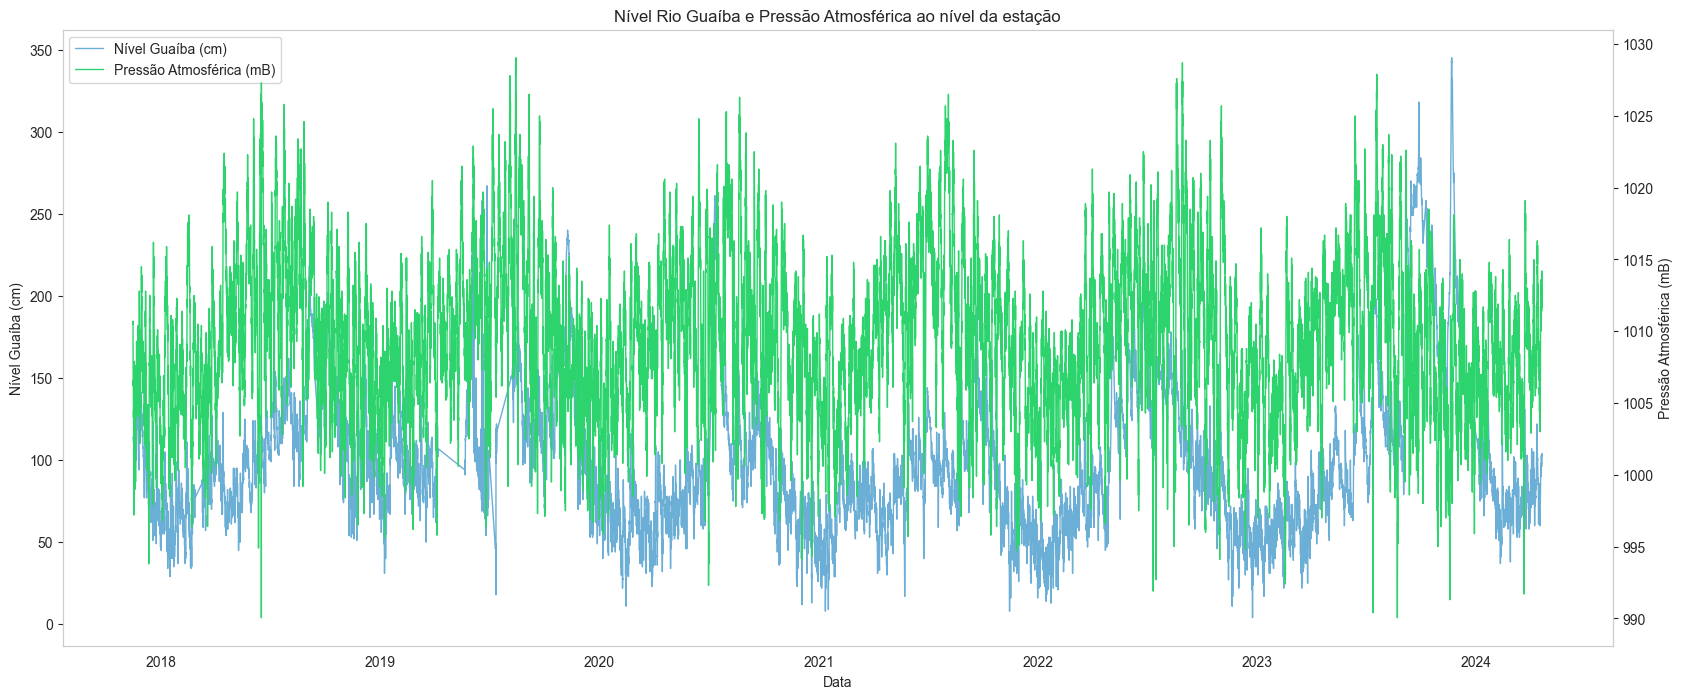
\includegraphics[scale=0.35]{figuras/comparacao_pressao_nivel_rio.png}
	\end{center}
	\fonte{Autor.}
\end{figure}

\begin{figure}[H]
	\caption{\label{fig:comparacao_radiacao_nivel_rio}Gráfico comparativo de radiação global e nível quanto a sazonalidade}
	\begin{center}
		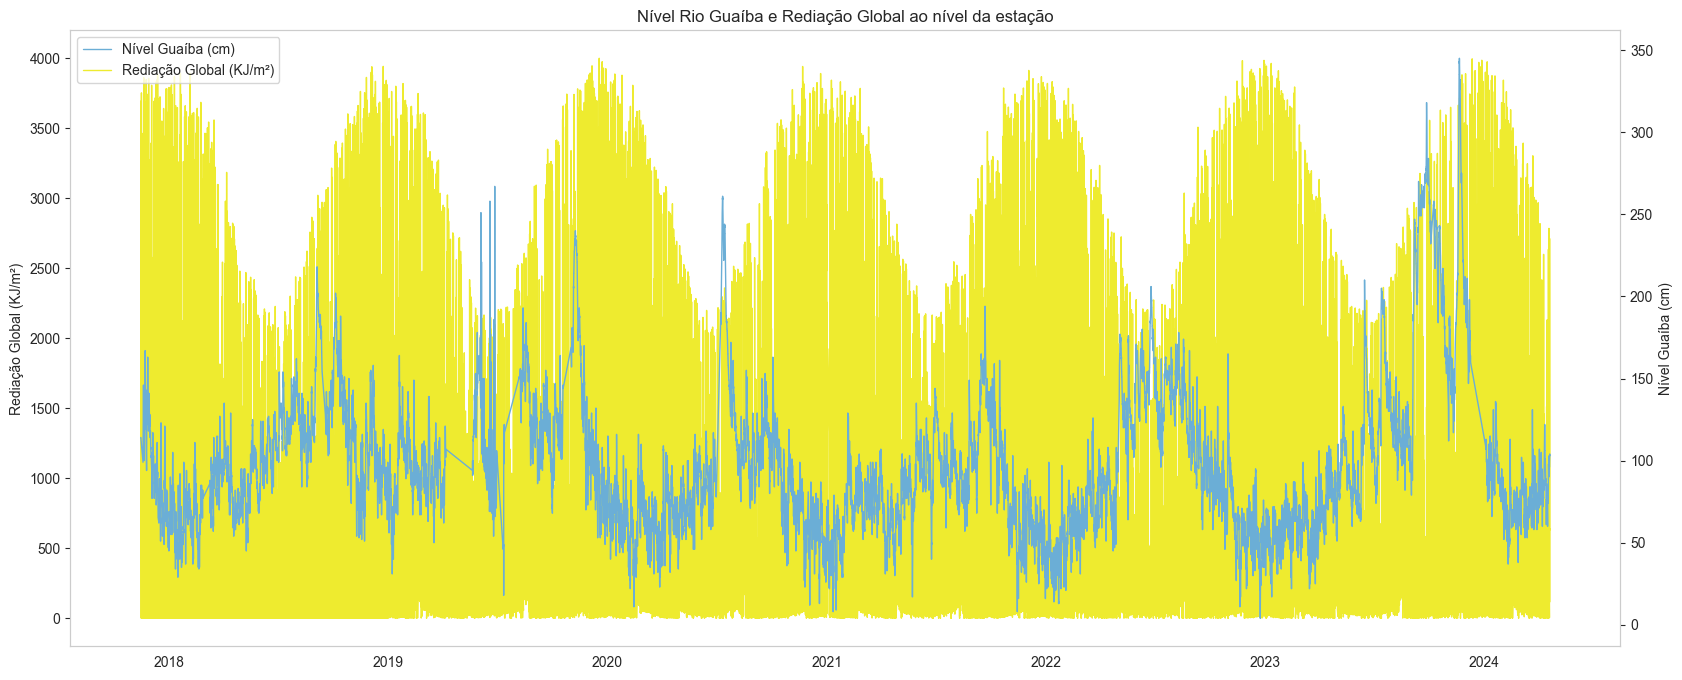
\includegraphics[scale=0.35]{figuras/comparacao_radiacao_nivel_rio.png}
	\end{center}
	\fonte{Autor.}
\end{figure}

Em relação às colunas \textit{Vento - Velocidade Horária}, \textit{Umidade Relativa do Ar} e \textit{Precipitação Total}, embora estas não apresentem um padrão sazonal tão evidente quanto as plotadas acima, estas medidas estão diretamente ligadas aos fenômenos de previsão do tempo, noticiadas em jornais e revistas, e portanto, possuem influência direta no nível dos rios ondes estes dados são monitorados. Sendo assim, as colunas também foram consideradas para o treinamento do modelo.

Definidas as colunas a serem mantidas, o próximo passo consistiu em alinhar os dados meteorológicos com os dados de monitoramento dos rios, garantindo que as informações estivessem na mesma frequência de amostragem. Para isso, foram utilizados os dados de monitoramento do nível do rio Guaíba, que possuem a maior frequência de amostragem entre os rios analisados, com intervalo de 15 minutos, enquanto os dados meteorológicos possuem frequência de 1 hora (60 minutos). Assim, a frequência de amostragem das informações do nível dos rios foi reduzida para 1 hora, aplicando um filtro simples que mantém apnas as linhas cujo \textit{timestamp} tem minuto igual a 0.

Por fim, alinhados os dados meteorológicos com os dados de monitoramento dos rios, o \textit{dataframe} resultante passou um nivelamento superior e inferior quanto a data inicial e final, de modo que o período de amostragem de todas as informações fosse o mesmo, garantindo que todas as colunas tivessem o mesmo número de linhas preenchidas. Embora na etapa de limpeza dos dados tenha sido aplicado o preenchimento de valores ausentes, verificou-se que as estações de monitoramento dos rios não possuem medições que se iniciam ou finalizam na mesma data. Dessa forma, a fim de analisar qual o período de início de fim das informações obtidas, a tabela \ref{tab:periodo_amostragem} apresenta o período de amostragem de cada uma das fontes de dados.
\begin{table}[H]
	\centering
	\begin{tabular}{|l|c|c|c|c|}
	\hline
	\textbf{Rio} & \textbf{Data Mínima} & \textbf{Hora Mínima} & \textbf{Data Máxima} & \textbf{Hora Máxima} \\
	\hline
	Rio dos Sinos & 2013-12-13 & 05:00:00 & 2024-06-30 & 09:00:00 \\
	Rio Caí       & 2015-09-14 & 13:00:00 & 2024-05-06 & 14:00:00 \\
	Rio Gravataí  & 2017-11-07 & 12:00:00 & 2024-07-01 & 00:00:00 \\
	Rio Jacuí     & 2014-10-08 & 20:00:00 & 2024-04-27 & 01:00:00 \\
	Rio Guaíba    & 2014-07-29 & 14:00:00 & 2024-05-06 & 14:00:00 \\
	\hline
	\end{tabular}
	\caption{Datas mínima e máxima disponíveis para cada rio analisado}
	\label{tab:periodo_amostragem}
\end{table}

Quanto a base de dados meteorológicos, o site do INMET disponibiliza dados desde o início dos anos 2000 e mantém a base atualizada até os dias atuais, não sendo, portanto, um limitador para a definição do período do dataframe final. Assim, o período de amostragem final pode ser definido a partir de 07 de novembro de 2017, que é a data mínima do rio Gravataí, até 06 de maio de 2024, que é a data máxima do rio Caí, com um dataframe de 56366 linhas.

\section{Transformação dos dados}

A transformação dos dados é uma etapa fundamental para garantir que as informações estejam no formato correto para o treinamento do modelo de previsão. Nesta fase, os dados são convertidos em um formato numérico, adequado para algoritmos de aprendizado de máquina, e normalizados para assegurar que todas as variáveis tenham a mesma escala.

Com os dados meteorológicos e de monitoramento dos rios alinhados, a normalização dos dados é aplicada visando principalmente equilibrar os dados dos níveis dos rios com os dados meteorológicos, tendo em vista que as escalas entre essas informações apresentam uma discrepância maior, pela diferença de unidade de medida entre elas.

Ademais, outro fator que deve ser considerado é se as colunas do \textit{dataframe} são compostas de dados categóricos (geralmente representados através de textos) ou numéricos. Por se tratar de medições aferidas por sensores meteorológicos e/ou geográficos, todas as colunas da base de dados estudada são numéricas.

A partir dessa premissa, a normalização dos dados foi feita utilizando o método \textit{StandardScaler} da biblioteca \textit{Scikit-learn}, que transforma os dados de uma coluna para um valor cuja média seja zero e desvio padrão igual a um. A pontuação padrão de uma amostra x é dada por:

\begin{equation}
z = \frac{x - \mu}{\sigma}
\end{equation}

onde \( \mu \) é a média da amostra e \( \sigma \) é o desvio padrão. Muitos elementos usados em funções objetivas de um algoritmo de aprendizagem (como o kernel RBF do Support Vector e as máquinas ou os regularizadores L1 e L2 dos modelos lineares) assumem que todos os recursos estão centrados em torno uma média igual a zero e variação de mesma ordem \cite{scikit_learn_standardscaler}. Desse modo, caso uma amostra apresente uma variância de magnitude maior do que outros, ele pode dominar a função objetivo e fazer o estimador incapaz de aprender com outros recursos corretamente como esperado.

Além disso, o método aplicado também é sensível a outliers, que afetam a média e o desvio padrão calculados para a definição dos valores normalizados. Por esse motivo, na seção \ref{sec:limpeza_dos_dados}, a aplicação do método IQR para remoção dos \textit{outliers}, além de limpar os dados durante aquela etapa de preparação, garantiu que os dados estivessem mais homogêneos e não fossem distorcidos por valores extremos na normalização desta etapa.

Para exemplificar a normalização dos dados, 

Com os dados normalizados, o \textit{dataframe} está pronto para ser dividido em conjuntos de treinamento e teste, chegando ao estágio final de preparação, e seguindo para o treinamento do modelo de previsão. 

\section{Divisão dos dados em conjuntos de treinamento e teste}

No processo de implementação de um modelo de previsão, a divisão da base de dados em conjuntos de treino e teste constitui a última etapa antes da aplicação do algoritmo, com o objetivo de avaliar a capacidade de generalização do modelo. De maneira geral, a base de dados é dividida em duas partes: uma maior, utilizada para o treinamento do modelo, e uma menor, destinada a testar seu desempenho em dados não observados durante o treinamento. Após a etapa de treinamento com o primeiro conjunto, é possível realizar previsões e compará-las com o segundo conjunto, cujos dados são conhecidos apenas pelo pesquisador. Essa comparação permite a avaliação da performance do modelo por meio do levantamento de métricas de desempenho.

Existem diferentes abordagens para dividir os dados em conjuntos de treinamento e teste, a fim de assegurar um bom desempenho do modelo de previsão. Por exemplo, em um estudo direcionado para a previsão do preço de ações, três proporções de divisão entre dados de treinamento e dados de teste foram aplicados, sendo estes:

\begin{itemize}
	\item 80\% dos dados para treinamento e 20\% para teste;
	\item 70\% dos dados para treinamento e 30\% para teste;
	\item 60\% dos dados para treinamento e 40\% para teste.
\end{itemize}

Através das métricas de desempenho \glsxtrfull{RMSE}, \glsxtrfull{MSE}, \glsxtrfull{R2} e \glsxtrfull{MAE}, os resultados das três proporções foram comparadas, de modo que a diferença percentual média entre o preço de validação e o preço previsto para o próximo dia útil foi menor para a proporção 80:20, com uma diferença média de 1,3\% entre o preço original e o preço previsto, enquanto a proporção 70:30 apresentou uma diferença média de 1,9\% e a proporção 60:40, 1,8\% \cite{supri2023asian}.

Embora a proporção 80:20 tenha apresentado o melhor desempenho neste estudo, não há uma regra geral que defina a melhor divisão entre os conjuntos de treinamento e teste, pois essa escolha pode variar de acordo com o tipo de dado, o modelo utilizado e outros fatores específicos de cada conjunto de informações. No presente trabalho, foi inicialmente adotada a proporção 80:20, com 80\% dos dados para treinamento e 20\% para teste, seguindo a abordagem utilizada no estudo mencionado, que obteve os melhores resultados. Para comparar o desempenho do modelo com outras proporções, também foram testadas as divisões 70:30 e 60:40, a fim de verificar se as métricas de desempenho apresentavam o mesmo comportamento observado no estudo de previsão de preços de ações.

\section{Aplicação do modelo de previsão}

Realizada toda a preparação dos dados, com a divisão em conjuntos de treino e teste e e a padronização das variáveis independentes para garantir que todas tenham a mesma escala, o modelo Ridge é instanciado no script em Python, com a possibilidade de ajuste de alguns parâmetros para fazer o treinamento e as previsões.

O principal parâmetro ajustável é o \texttt{alpha}, que controla a intensidade da penalização: valores maiores de \texttt{alpha} aumentam a regularização, reduzindo a magnitude dos coeficientes, podendo levar a underfitting; valores menores aproximam o modelo da regressão linear padrão, com risco de overfitting. Outros parâmetros incluem \texttt{fit\_intercept}, que determina se o modelo deve incluir um intercepto, e \texttt{solver}, que define o método de otimização (como \texttt{auto}, \texttt{svd} ou \texttt{cholesky}), influenciando a eficiência computacional. Além disso, o parâmetro \texttt{random\_state} pode ser configurado para garantir reprodutibilidade em solvers que utilizam aleatoriedade.

A implementação prática envolve importar a classe Ridge, configurar os hiperparâmetros, treinar o modelo com o método \texttt{fit} e realizar previsões com o método \texttt{predict}. Para avaliar o desempenho do modelo, esta etapa é feita com métricas como o erro quadrático médio (MSE), raíz do erro quadrático médio (RMSE), erro absoluto médio (MAE) e/ou o coeficiente de determinação (R²).

Em \cite{Hastie01102020}, o autor aborda sobre o termo de regularização L2 que penaliza os coeficientes do modelo, explorando o impacto do parâmetro \texttt{alpha} em vários contextos. Em sua tese, é destacado que valores de \texttt{alpha} são geralmente selecionados por validação cruzada, com intervalos típicos variando de 0.01 a 1000, dependendo da escala dos dados e do grau de multicolinearidade. O artigo também menciona que, em aplicações práticas, valores como 0.1, 1 e 10 são frequentemente testados como pontos de partida.

Partindo desse pressuposto, foram testados valores de \texttt{alpha} de 0.001, 0.01, 0.1, 1, 10 e 100, com o objetivo de avaliar o desempenho do modelo em diferentes níveis de regularização. A seguir, são apresentadas as tabelas com os resultados obtidos para cada valor de \texttt{alpha}, considerando as três proporções de divisão dos dados em conjuntos de treinamento e teste: 80:20, 70:30 e 60:40, junto às Figuras X, Y e Z, que ilustram o desempenho do modelo para cada split de treinamento e previsão.

\begin{figure}[H]
	\caption{\label{fig:comparacao_radiacao_nivel_rio}Gráfico modelo de previsão de nível do rio Guaíba com \texttt{alpha} = 1 e split de treinamento e teste 60:40}
	\begin{center}
		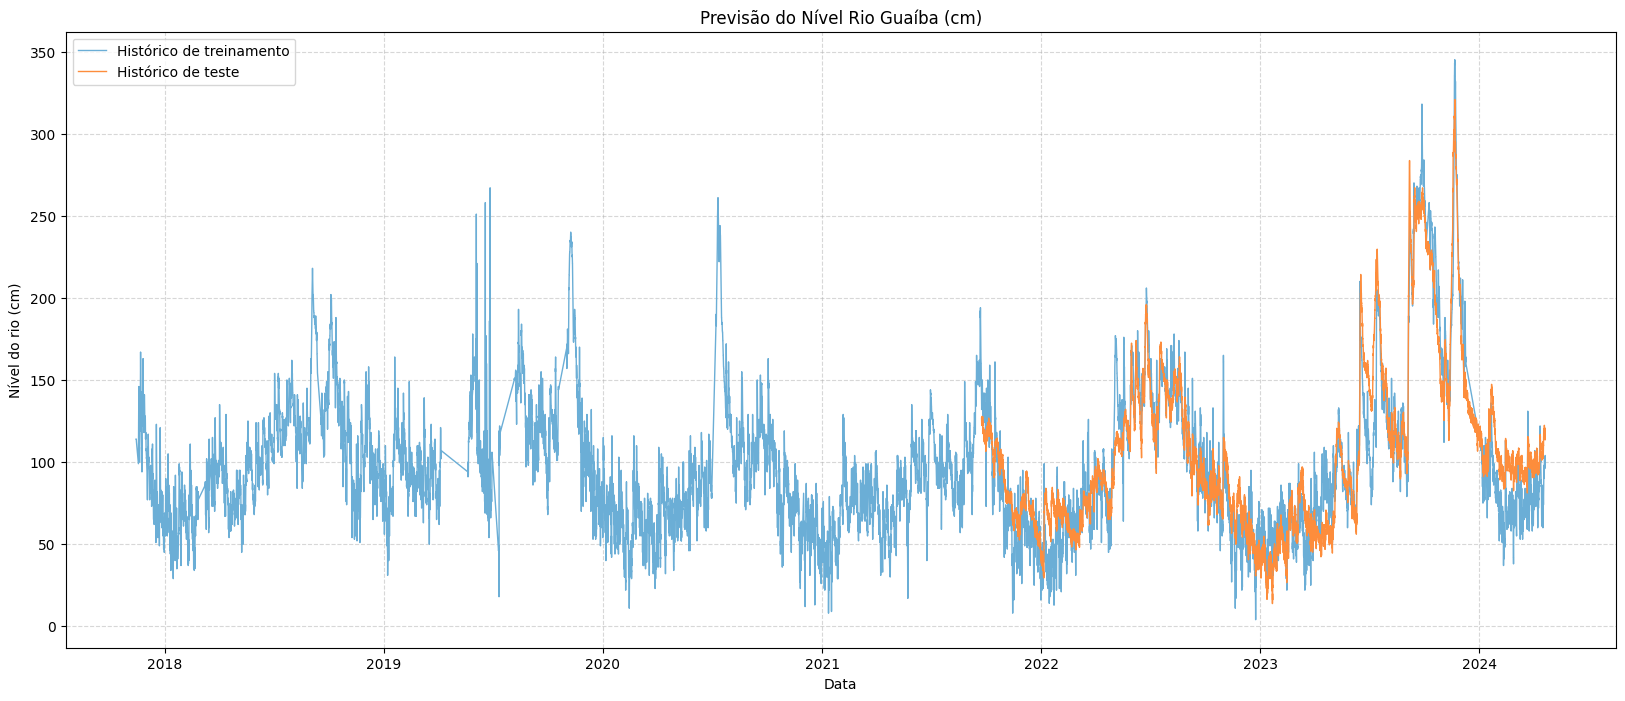
\includegraphics[scale=0.35]{figuras/modelo_previsao_60_40.png}
	\end{center}
	\fonte{Autor.}
\end{figure}

\begin{figure}[H]
	\caption{\label{fig:comparacao_radiacao_nivel_rio}Gráfico modelo de previsão de nível do rio Guaíba com \texttt{alpha} = 1 e split de treinamento e teste 70:30}
	\begin{center}
		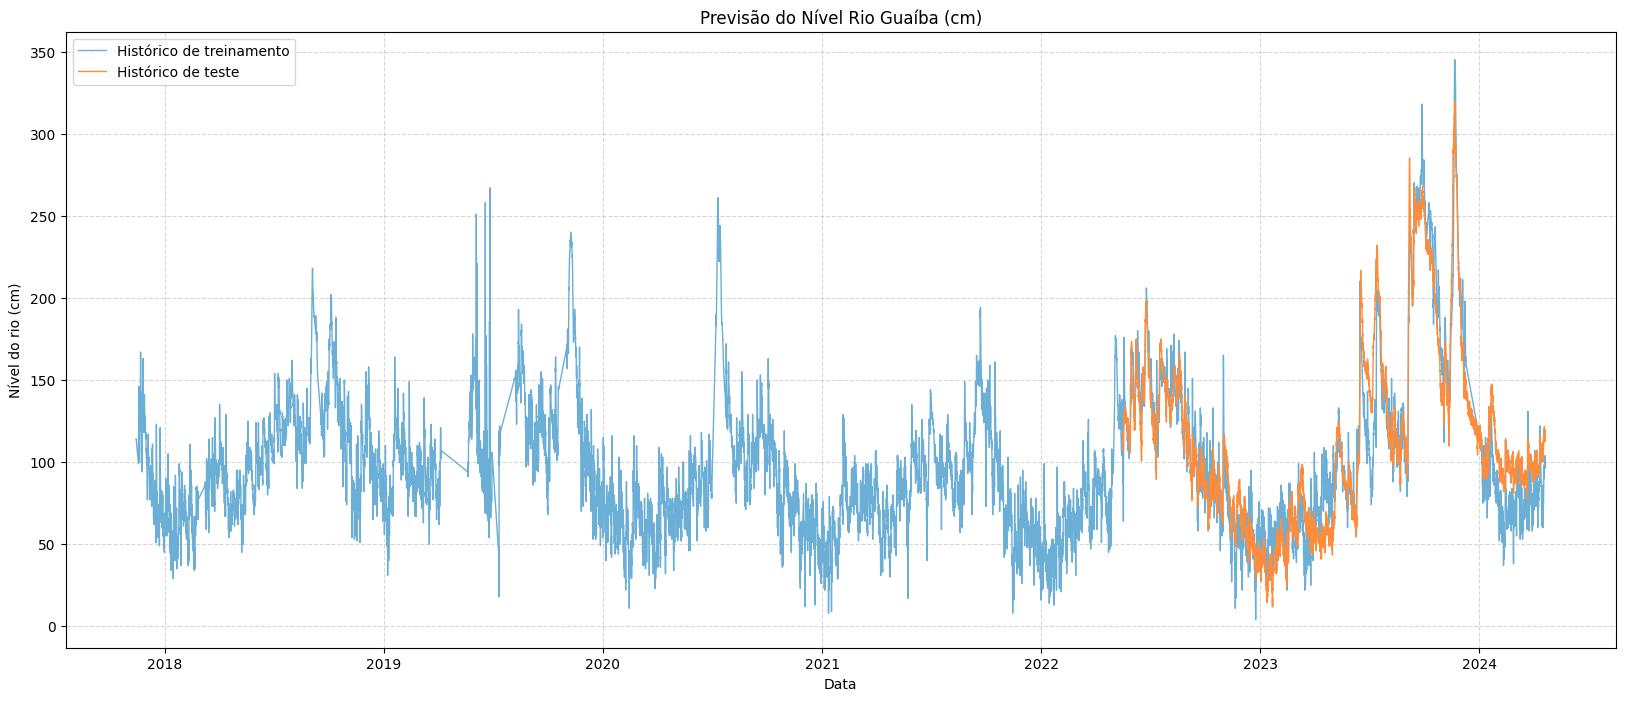
\includegraphics[scale=0.35]{figuras/modelo_previsao_70_30.png}
	\end{center}
	\fonte{Autor.}
\end{figure}

\begin{figure}[H]
	\caption{\label{fig:comparacao_radiacao_nivel_rio}Gráfico modelo de previsão de nível do rio Guaíba com \texttt{alpha} = 1 e split de treinamento e teste 80:20}
	\begin{center}
		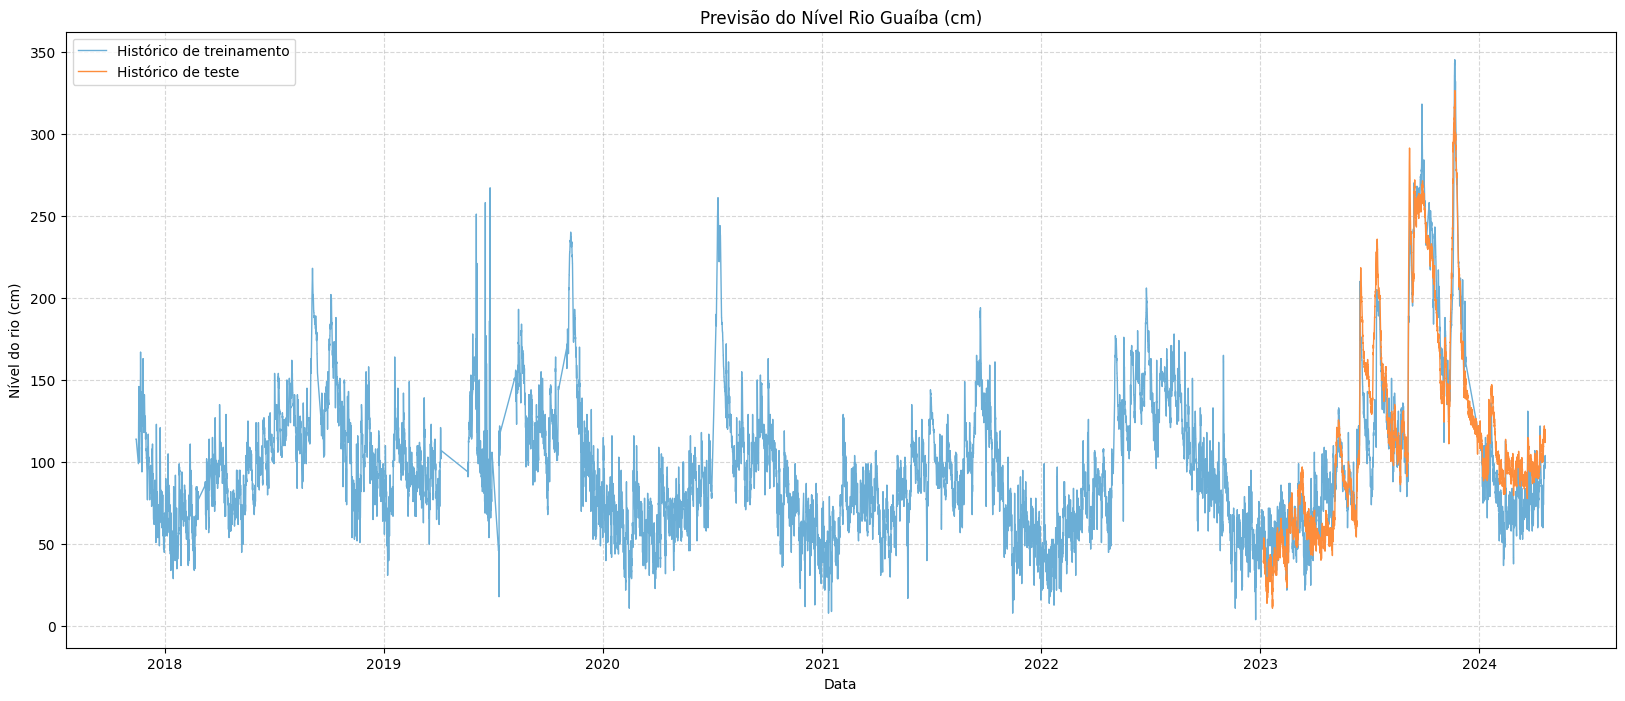
\includegraphics[scale=0.35]{figuras/modelo_previsao_80_20.png}
	\end{center}
	\fonte{Autor.}
\end{figure}

\begin{table}[H]
\centering
\begin{tabular}{|c|c|c|c|c|}
\hline
\textbf{Alpha} & \multicolumn{4}{|c|}{\textbf{0.001}} \\
\hline
\textbf{Split} & \textbf{MSE} & \textbf{RMSE} & \textbf{MAE} & \textbf{R2} \\
\hline
\textbf{80:20} & 456.72 & 21.27 & 16.81 & 0.89 \\
\textbf{70:30} & 372.44 & 19.30 & 15.00 & 0.88 \\
\textbf{60:40} & 379.64 & 19.48 & 15.14 & 0.87 \\
\hline
\end{tabular}
\caption{Tabela de avaliação de desempenho do modelo com alpha 0.01}
\end{table}

\begin{table}[H]
\centering
\begin{tabular}{|c|c|c|c|c|}
\hline
\textbf{Alpha} & \multicolumn{4}{|c|}{\textbf{0.001}} \\
\hline
\textbf{Split} & \textbf{MSE} & \textbf{RMSE} & \textbf{MAE} & \textbf{R2} \\
\hline
\textbf{80:20} & 456.72 & 21.27 & 16.81 & 0.89 \\
\textbf{70:30} & 372.44 & 19.30 & 15.00 & 0.88 \\
\textbf{60:40} & 379.64 & 19.48 & 15.14 & 0.87 \\
\hline
\end{tabular}
\caption{Tabela de avaliação de desempenho do modelo com alpha 0.1}
\end{table}

\begin{table}[H]
\centering
\begin{tabular}{|c|c|c|c|c|}
\hline
\textbf{Alpha} & \multicolumn{4}{|c|}{\textbf{0.001}} \\
\hline
\textbf{Split} & \textbf{MSE} & \textbf{RMSE} & \textbf{MAE} & \textbf{R2} \\
\hline
\textbf{80:20} & 456.72 & 21.27 & 16.81 & 0.89 \\
\textbf{70:30} & 372.44 & 19.30 & 15.00 & 0.88 \\
\textbf{60:40} & 379.65 & 19.48 & 15.14 & 0.87 \\
\hline
\end{tabular}
\caption{Tabela de avaliação de desempenho do modelo com alpha 1}
\end{table}

\begin{table}[H]
\centering
\begin{tabular}{|c|c|c|c|c|}
\hline
\textbf{Alpha} & \multicolumn{4}{|c|}{\textbf{0.001}} \\
\hline
\textbf{Split} & \textbf{MSE} & \textbf{RMSE} & \textbf{MAE} & \textbf{R2} \\
\hline
\textbf{80:20} & 456.72 & 21.27 & 16.81 & 0.89 \\
\textbf{70:30} & 372.44 & 19.30 & 15.00 & 0.88 \\
\textbf{60:40} & 379.64 & 19.48 & 15.14 & 0.87 \\
\hline
\end{tabular}
\caption{Tabela de avaliação de desempenho do modelo com alpha 10}
\end{table}

\begin{table}[H]
\centering
\begin{tabular}{|c|c|c|c|c|}
\hline
\textbf{Alpha} & \multicolumn{4}{|c|}{\textbf{0.001}} \\
\hline
\textbf{Split} & \textbf{MSE} & \textbf{RMSE} & \textbf{MAE} & \textbf{R2} \\
\hline
\textbf{80:20} & 456.73 & 21.27 & 16.81 & 0.89 \\
\textbf{70:30} & 372.45 & 19.30 & 15.00 & 0.88 \\
\textbf{60:40} & 379.65 & 19.48 & 15.14 & 0.87 \\
\hline
\end{tabular}
\caption{Tabela de avaliação de desempenho do modelo com alpha 100}
\end{table}


\section{Análise dos resultados}

Uma das formas de avaliar o desempenho de um modelo de aprendizado de máquina é através da análise das métricas de desempenho, que indicam a capacidade do modelo de generalizar e prever corretamente os dados. As métricas de avaliação utilizadas neste trabalho incluem o erro quadrático médio (MSE), a raiz do erro quadrático médio (RMSE), o erro absoluto médio (MAE) e o coeficiente de determinação (R²), onde cada uma delas possui uma interpretação específica:

\begin{itemize}
	\item Erro Quadrático Médio (MSE): Mede a média dos quadrados dos erros, penalizando erros maiores. É útil para entender a magnitude do erro, porém não é intuitiva em termos da escala dos dados, neste caso medido em centímetros.
	\item Raiz do Erro Quadrático Médio (RMSE): É a raiz quadrada do MSE, expressa na mesma unidade dos dados, facilitando a interpretação.
	\item Erro Absoluto Médio (MAE): Mede a média dos erros absolutos, sendo menos sensível a outliers do que o MSE.
	\item R² (Coeficiente de Determinação): Indica a proporção da variância dos dados explicada pelo modelo. Varia de 0 a 1, onde 1 significa ajuste perfeito.
\end{itemize}

Com isso, as tabelas apresentadas mostram que o MSE e o RMSE diminuem conforme o \textit{split} de treinamento diminui e o \textit{split} de teste aumenta. Tal comportamento indica que, à medida que mais dados são utilizados para treinamento, o modelo passa a ter um sobreajuste (\textit{overfitting}), perdendo a capacidade de generalizar e, em vez disso, se adequando estritamente ao conjunto de dados de treinamento.

Quanto ao R², o valor obtido possui uma baixa variação entre os ensaios com diferentes valores de \texttt{alpha} e \textit{split}, ficando entre 0.87 e 0.89. Isso indica que 87\% a 89\% da variância dos dados da variável dependente é explicada pelo modelo. Em outras palavras, o modelo captura a maior parte dos padrões nos dados, deixando apenas 13\% a 11\% da variância como não explicada (devido a ruído, variáveis omitidas ou outros fatores).

Um coeficiente de determinação próximo a 1 sugere que o modelo é robusto e confiável para o conjunto de dados analisado. Boa parte dessa robustez se dá pelo tratamento e limpeza dos dados, somada à a correlação entre as variáveis preditoras e a variável dependente.

Em relação ao parâmetro \texttt{alpha}, os resultados mostram que o modelo apresenta um desempenho semelhante para os valores de 0.001, 0.01, 0.1 e 1, com pequenas variações nas métricas de desempenho. Existem alguns fatores que levam a esse comportamento, como a baixa sensibilidade à regularização nos dados, intervalo de \texttt{alpha} insuficiente para notar diferenças significativas ou baixa multicolinearidade entre as variáveis preditoras. Alguns outros fatores como escala dos dados ou tamanho e qualidade do conjunto foi descartado, uma vez que ao longo do trabalho, evidenciam-se os procedimentos realizados para evitar este tipo de falha no modelo.

Sendo assim, uma forma de testar se o modelo possui uma sensibilidade maior à regularização seria aumentar o intervalo de valores de \texttt{alpha} e/ou expor o modelo a mais dados de teste. Caso a variação de \texttt{alpha} permaneça com resultados semelhantes, isto pode indicar que o modelo já atingiu seu ponto de saturação, atingindo um desempenho ótimo para baixos termos de regularização.
	
	% 4 - Conclusão
	% ----------------------------------------------------------
\chapter{Conclusão}
% ----------------------------------------------------------
O presente trabalho teve como objetivo geral desenvolver um modelo de previsão do nível do Lago Guaíba, utilizando dados meteorológicos por meio da técnica de Regressão Ridge. Para alcançar esse propósito, foram estabelecidos objetivos específicos que envolveram desde a coleta e pré-processamento dos dados, até a implementação do modelo e análise dos resultados.

No desenvolvimento do projeto, procedeu-se à coleta de dados meteorológicos disponibilizados pelo INMET, assim como dos níveis hidrométricos dos rios da bacia do Guaíba, através do SEMA-RS. Esses dados passaram por um pré-processamento, que incluiu a limpeza, tratamento de valores ausentes, remoção de outliers e normalização, garantindo maior qualidade ao conjunto utilizado para treinamento. Foi também realizada a redução da dimensionalidade, mantendo apenas variáveis com maior relevância para a previsão, como temperatura do ar, pressão atmosférica, radiação global, velocidade do vento, umidade relativa e precipitação.

Na etapa de implementação, o modelo de Regressão Ridge foi escolhido por sua capacidade de lidar com multicolinearidade e reduzir o risco de sobreajuste, característica importante considerando a volatilidade das variáveis climáticas. Foram testados diferentes valores do parâmetro de regularização (\texttt{alpha}), variando também as proporções de divisão entre conjuntos de treinamento e teste (80:20, 70:30, 60:40). Para avaliar o desempenho da previsão do modelo, as métricas de desempenho — MSE, RMSE, MAE e R² foram utilizadas, visando uma análise mais objetiva e estatística da implementação.

Os resultados evidenciaram a robustez do modelo e a correlação significativa entre variáveis meteorológicas e o nível do Lago Guaíba. Apesar de pequenas variações nos indicadores de desempenho, não se observou impacto expressivo da alteração dos valores de alpha, sugerindo que o modelo atinge um platô de desempenho para os intervalos testados. Tal constatação indica que ajustes adicionais de regularização, ou a inclusão de novas variáveis externas, poderiam ser explorados em trabalhos futuros para ganhos incrementais de performance. Além disso, cabe a comparação com outros modelos de previsão existentes, ou até mesmo uma rede neural para comparar o desempenho em relação ao modelo Ridge.

Assim, conclui-se que o objetivo proposto foi atingido. O modelo desenvolvido mostrou-se eficiente e tecnicamente sólido para prever o nível do Lago Guaíba a partir dos dados meteorológicos utilizados. Entretanto, vale ressaltar que os dados utilizados são históricos, ou seja, compõem medidas meteorológicas aferidas por instrumentos no momento da medição. Para uma aplicação real de previsão do nível do rio, visando um alerta antecipado de enchente, o modelo seria expostos a medidas meteorológicas previstas ao invés de medidas, adicionando um grau de incerteza que pode gerar previsões com um grau de erro maior. Por isso, é necessário realizar testes com dados previstos, avaliar novas métricas de desempenho, para então considerar o uso do modelo em casos reais de previsão do nível do rio.  
	
	
	% Elementos pós-textuais
	\postextual
	
	
	% Referências bibliográficas
	\begingroup
	    \printbibliography[title=REFERÊNCIAS]
	\endgroup
	
	
	
	%Reconfiguração do título para apêndices e anexos
	 \renewcommand{\ABNTEXchapterupperifneeded}[1]{#1} 
	\makeatletter
	\settocpreprocessor{chapter}{%
      \let\tempf@rtoc\f@rtoc%
      \def\f@rtoc{%
      \texorpdfstring{{\tempf@rtoc}}{\tempf@rtoc}}%
      }
    \makeatother
	
	
	% Apêndices
    \begin{apendicesenv}
    	%\partapendices* 
    	% ----------------------------------------------------------
\chapter{Descrição}   %Apenas a primeira letra deve ser maiúscula
% ----------------------------------------------------------

Textos elaborados pelo autor, a fim de completar a sua argumentação. Deve ser precedido da palavra APÊNDICE, identificada por letras maiúsculas consecutivas, travessão e pelo respectivo título. Utilizam-se letras maiúsculas dobradas quando esgotadas as letras do alfabeto. 

    \end{apendicesenv}

    % Anexos
    \begin{anexosenv}
    	%\partanexos*
    	% ----------------------------------------------------------
\chapter{Descrição}   %Apenas a primeira letra deve ser maiúscula
% ----------------------------------------------------------

São documentos não elaborados pelo autor que servem como fundamentação (mapas, leis, estatutos). Deve ser precedido da palavra ANEXO, identificada por letras maiúsculas consecutivas, travessão e pelo respectivo título. Utilizam-se letras maiúsculas dobradas quando esgotadas as letras do alfabeto. 

    \end{anexosenv}

\end{document}